%%%%%%%%%%%%%%%%%%%%%%%%%%%%%%%%%%%%%%%%%
% The Legrand Orange Book
% LaTeX Template
% Version 2.1.1 (14/2/16)
%
% This template has been downloaded from:
% http://www.LaTeXTemplates.com
%
% Original author:
% Mathias Legrand (legrand.mathias@gmail.com) with modifications by:
% Vel (vel@latextemplates.com)
%
% License:
% CC BY-NC-SA 3.0 (http://creativecommons.org/licenses/by-nc-sa/3.0/)
%
% Compiling this template:
% This template uses biber for its bibliography and makeindex for its index.
% When you first open the template, compile it from the command line with the 
% commands below to make sure your LaTeX distribution is configured correctly:
%
% 1) pdflatex main
% 2) makeindex main.idx -s StyleInd.ist
% 3) biber main
% 4) pdflatex main x 2
%
% After this, when you wish to update the bibliography/index use the appropriate
% command above and make sure to compile with pdflatex several times 
% afterwards to propagate your changes to the document.
%
% This template also uses a number of packages which may need to be
% updated to the newest versions for the template to compile. It is strongly
% recommended you update your LaTeX distribution if you have any
% compilation errors.
%
% Important note:
% Chapter heading images should have a 2:1 width:height ratio,
% e.g. 920px width and 460px height.
%
%%%%%%%%%%%%%%%%%%%%%%%%%%%%%%%%%%%%%%%%%

%----------------------------------------------------------------------------------------
%	PACKAGES AND OTHER DOCUMENT CONfigureTIONS
%----------------------------------------------------------------------------------------

\documentclass[12pt,fleqn]{book} % Default font size and left-justified equations
\usepackage{enumerate}
\usepackage{quoting}
\usepackage{setspace}

%----------------------------------------------------------------------------------------

%%%%%%%%%%%%%%%%%%%%%%%%%%%%%%%%%%%%%%%%%
% The Legrand Orange Book
% Structural Definitions File
% Version 2.0 (9/2/15)
%
% Original author:
% Mathias Legrand (legrand.mathias@gmail.com) with modifications by:
% Vel (vel@latextemplates.com)
% 
% This file has been downloaded from:
% http://www.LaTeXTemplates.com
%
% License:
% CC BY-NC-SA 3.0 (http://creativecommons.org/licenses/by-nc-sa/3.0/)
%
%%%%%%%%%%%%%%%%%%%%%%%%%%%%%%%%%%%%%%%%%

%----------------------------------------------------------------------------------------
%	VARIOUS REQUIRED PACKAGES AND CONFIGURATIONS
%----------------------------------------------------------------------------------------

\usepackage[top=3cm,bottom=3cm,left=3cm,right=3cm,headsep=10pt,a4paper]{geometry} % Page margins

\usepackage{graphicx} % Required for including pictures
\graphicspath{{Pictures/}} % Specifies the directory where pictures are stored

\usepackage{lipsum} % Inserts dummy text

\usepackage{tikz} % Required for drawing custom shapes

\usepackage[english]{babel} % English language/hyphenation

\usepackage{enumitem} % Customize lists
\setlist{nolistsep} % Reduce spacing between bullet points and numbered lists

\usepackage{booktabs} % Required for nicer horizontal rules in tables

\usepackage{xcolor} % Required for specifying colors by name
\definecolor{ocre}{RGB}{243,102,25} % Define the orange color used for highlighting throughout the book

%----------------------------------------------------------------------------------------
%	FONTS
%----------------------------------------------------------------------------------------

\usepackage{avant} % Use the Avantgarde font for headings
%\usepackage{times} % Use the Times font for headings
\usepackage{mathptmx} % Use the Adobe Times Roman as the default text font together with math symbols from the Sym­bol, Chancery and Com­puter Modern fonts

\usepackage{microtype} % Slightly tweak font spacing for aesthetics
\usepackage[utf8]{inputenc} % Required for including letters with accents
\usepackage[T1]{fontenc} % Use 8-bit encoding that has 256 glyphs

%----------------------------------------------------------------------------------------
%	BIBLIOGRAPHY AND INDEX
%----------------------------------------------------------------------------------------

\usepackage{csquotes}
\usepackage[style=authoryear,citestyle=authoryear,sorting=nyt,sortcites=true,autopunct=true,autolang=hyphen,hyperref=true,abbreviate=false,backref=true,backend=bibtex,defernumbers=true]{biblatex}
\addbibresource{bibliography.bib} % BibTeX bibliography file
\defbibheading{bibempty}{}

\usepackage{calc} % For simpler calculation - used for spacing the index letter headings correctly
\usepackage{makeidx} % Required to make an index
\makeindex % Tells LaTeX to create the files required for indexing

%----------------------------------------------------------------------------------------
%	MAIN TABLE OF CONTENTS
%----------------------------------------------------------------------------------------

\usepackage{titletoc} % Required for manipulating the table of contents

\contentsmargin{0cm} % Removes the default margin

% Part text styling
\titlecontents{part}[0cm]
{\addvspace{20pt}\centering\large\bfseries}
{}
{}
{}

% Chapter text styling
\titlecontents{chapter}[1.25cm] % Indentation
{\addvspace{12pt}\large\sffamily\bfseries} % Spacing and font options for chapters
{\color{ocre!60}\contentslabel[\Large\thecontentslabel]{1.25cm}\color{ocre}} % Chapter number
{\color{ocre}}  
{\color{ocre!60}\normalsize\;\titlerule*[.5pc]{.}\;\thecontentspage} % Page number

% Section text styling
\titlecontents{section}[1.25cm] % Indentation
{\addvspace{3pt}\sffamily\bfseries} % Spacing and font options for sections
{\contentslabel[\thecontentslabel]{1.25cm}} % Section number
{}
{\hfill\color{black}\thecontentspage} % Page number
[]

% Subsection text styling
\titlecontents{subsection}[1.25cm] % Indentation
{\addvspace{1pt}\sffamily\small} % Spacing and font options for subsections
{\contentslabel[\thecontentslabel]{1.25cm}} % Subsection number
{}
{\ \titlerule*[.5pc]{.}\;\thecontentspage} % Page number
[]

% List of figures
\titlecontents{figure}[0em]
{\addvspace{-5pt}\sffamily}
{\thecontentslabel\hspace*{1em}}
{}
{\ \titlerule*[.5pc]{.}\;\thecontentspage}
[]

% List of tables
\titlecontents{table}[0em]
{\addvspace{-5pt}\sffamily}
{\thecontentslabel\hspace*{1em}}
{}
{\ \titlerule*[.5pc]{.}\;\thecontentspage}
[]

%----------------------------------------------------------------------------------------
%	MINI TABLE OF CONTENTS IN PART HEADS
%----------------------------------------------------------------------------------------

% Chapter text styling
\titlecontents{lchapter}[0em] % Indenting
{\addvspace{15pt}\large\sffamily\bfseries} % Spacing and font options for chapters
{\color{ocre}\contentslabel[\Large\thecontentslabel]{1.25cm}\color{ocre}} % Chapter number
{}  
{\color{ocre}\normalsize\sffamily\bfseries\;\titlerule*[.5pc]{.}\;\thecontentspage} % Page number

% Section text styling
\titlecontents{lsection}[0em] % Indenting
{\sffamily\small} % Spacing and font options for sections
{\contentslabel[\thecontentslabel]{1.25cm}} % Section number
{}
{}

% Subsection text styling
\titlecontents{lsubsection}[.5em] % Indentation
{\normalfont\footnotesize\sffamily} % Font settings
{}
{}
{}

%----------------------------------------------------------------------------------------
%	PAGE HEADERS
%----------------------------------------------------------------------------------------

\usepackage{fancyhdr} % Required for header and footer configuration

\pagestyle{fancy}
\renewcommand{\chaptermark}[1]{\markboth{\sffamily\normalsize\bfseries\chaptername\ \thechapter.\ #1}{}} % Chapter text font settings
\renewcommand{\sectionmark}[1]{\markright{\sffamily\normalsize\thesection\hspace{5pt}#1}{}} % Section text font settings
\fancyhf{} \fancyhead[LE,RO]{\sffamily\normalsize\thepage} % Font setting for the page number in the header
\fancyhead[LO]{\rightmark} % Print the nearest section name on the left side of odd pages
\fancyhead[RE]{\leftmark} % Print the current chapter name on the right side of even pages
\renewcommand{\headrulewidth}{0.5pt} % Width of the rule under the header
\addtolength{\headheight}{2.5pt} % Increase the spacing around the header slightly
\renewcommand{\footrulewidth}{0pt} % Removes the rule in the footer
\fancypagestyle{plain}{\fancyhead{}\renewcommand{\headrulewidth}{0pt}} % Style for when a plain pagestyle is specified

% Removes the header from odd empty pages at the end of chapters
\makeatletter
\renewcommand{\cleardoublepage}{
\clearpage\ifodd\c@page\else
\hbox{}
\vspace*{\fill}
\thispagestyle{empty}
\newpage
\fi}

%----------------------------------------------------------------------------------------
%	THEOREM STYLES
%----------------------------------------------------------------------------------------

\usepackage{amsmath,amsfonts,amssymb,amsthm} % For math equations, theorems, symbols, etc

\newcommand{\intoo}[2]{\mathopen{]}#1\,;#2\mathclose{[}}
\newcommand{\ud}{\mathop{\mathrm{{}d}}\mathopen{}}
\newcommand{\intff}[2]{\mathopen{[}#1\,;#2\mathclose{]}}
\newtheorem{notation}{Notation}[chapter]

% Boxed/framed environments
\newtheoremstyle{ocrenumbox}% % Theorem style name
{0pt}% Space above
{0pt}% Space below
{\normalfont}% % Body font
{}% Indent amount
{\small\bf\sffamily\color{ocre}}% % Theorem head font
{\;}% Punctuation after theorem head
{0.25em}% Space after theorem head
{\small\sffamily\color{ocre}\thmname{#1}\nobreakspace\thmnumber{\@ifnotempty{#1}{}\@upn{#2}}% Theorem text (e.g. Theorem 2.1)
\thmnote{\nobreakspace\the\thm@notefont\sffamily\bfseries\color{black}---\nobreakspace#3.}} % Optional theorem note
\renewcommand{\qedsymbol}{$\blacksquare$}% Optional qed square

\newtheoremstyle{blacknumex}% Theorem style name
{5pt}% Space above
{5pt}% Space below
{\normalfont}% Body font
{} % Indent amount
{\small\bf\sffamily}% Theorem head font
{\;}% Punctuation after theorem head
{0.25em}% Space after theorem head
{\small\sffamily{\tiny\ensuremath{\blacksquare}}\nobreakspace\thmname{#1}\nobreakspace\thmnumber{\@ifnotempty{#1}{}\@upn{#2}}% Theorem text (e.g. Theorem 2.1)
\thmnote{\nobreakspace\the\thm@notefont\sffamily\bfseries---\nobreakspace#3.}}% Optional theorem note

\newtheoremstyle{blacknumbox} % Theorem style name
{0pt}% Space above
{0pt}% Space below
{\normalfont}% Body font
{}% Indent amount
{\small\bf\sffamily}% Theorem head font
{\;}% Punctuation after theorem head
{0.25em}% Space after theorem head
{\small\sffamily\thmname{#1}\nobreakspace\thmnumber{\@ifnotempty{#1}{}\@upn{#2}}% Theorem text (e.g. Theorem 2.1)
\thmnote{\nobreakspace\the\thm@notefont\sffamily\bfseries---\nobreakspace#3.}}% Optional theorem note

% Non-boxed/non-framed environments
\newtheoremstyle{ocrenum}% % Theorem style name
{5pt}% Space above
{5pt}% Space below
{\normalfont}% % Body font
{}% Indent amount
{\small\bf\sffamily\color{ocre}}% % Theorem head font
{\;}% Punctuation after theorem head
{0.25em}% Space after theorem head
{\small\sffamily\color{ocre}\thmname{#1}\nobreakspace\thmnumber{\@ifnotempty{#1}{}\@upn{#2}}% Theorem text (e.g. Theorem 2.1)
\thmnote{\nobreakspace\the\thm@notefont\sffamily\bfseries\color{black}---\nobreakspace#3.}} % Optional theorem note
\renewcommand{\qedsymbol}{$\blacksquare$}% Optional qed square
\makeatother

% Defines the theorem text style for each type of theorem to one of the three styles above
\newcounter{dummy} 
\numberwithin{dummy}{section}
\theoremstyle{ocrenumbox}
\newtheorem{theoremeT}[dummy]{Theorem}
\newtheorem{problem}{Problem}[chapter]
\newtheorem{exerciseT}{Exercise}[chapter]
\theoremstyle{blacknumex}
\newtheorem{exampleT}{Example}[chapter]
\theoremstyle{blacknumbox}
\newtheorem{vocabulary}{Vocabulary}[chapter]
\newtheorem{definitionT}{Definition}[section]
\newtheorem{corollaryT}[dummy]{Corollary}
\theoremstyle{ocrenum}
\newtheorem{proposition}[dummy]{Proposition}

%----------------------------------------------------------------------------------------
%	DEFINITION OF COLORED BOXES
%----------------------------------------------------------------------------------------

\RequirePackage[framemethod=default]{mdframed} % Required for creating the theorem, definition, exercise and corollary boxes

% Theorem box
\newmdenv[skipabove=7pt,
skipbelow=7pt,
backgroundcolor=black!5,
linecolor=ocre,
innerleftmargin=5pt,
innerrightmargin=5pt,
innertopmargin=5pt,
leftmargin=0cm,
rightmargin=0cm,
innerbottommargin=5pt]{tBox}

% Exercise box	  
\newmdenv[skipabove=7pt,
skipbelow=7pt,
rightline=false,
leftline=true,
topline=false,
bottomline=false,
backgroundcolor=ocre!10,
linecolor=ocre,
innerleftmargin=5pt,
innerrightmargin=5pt,
innertopmargin=5pt,
innerbottommargin=5pt,
leftmargin=0cm,
rightmargin=0cm,
linewidth=4pt]{eBox}	

% Definition box
\newmdenv[skipabove=7pt,
skipbelow=7pt,
rightline=false,
leftline=true,
topline=false,
bottomline=false,
linecolor=ocre,
innerleftmargin=5pt,
innerrightmargin=5pt,
innertopmargin=0pt,
leftmargin=0cm,
rightmargin=0cm,
linewidth=4pt,
innerbottommargin=0pt]{dBox}	

% Corollary box
\newmdenv[skipabove=7pt,
skipbelow=7pt,
rightline=false,
leftline=true,
topline=false,
bottomline=false,
linecolor=gray,
backgroundcolor=black!5,
innerleftmargin=5pt,
innerrightmargin=5pt,
innertopmargin=5pt,
leftmargin=0cm,
rightmargin=0cm,
linewidth=4pt,
innerbottommargin=5pt]{cBox}

% Creates an environment for each type of theorem and assigns it a theorem text style from the "Theorem Styles" section above and a colored box from above
\newenvironment{theorem}{\begin{tBox}\begin{theoremeT}}{\end{theoremeT}\end{tBox}}
\newenvironment{exercise}{\begin{eBox}\begin{exerciseT}}{\hfill{\color{ocre}\tiny\ensuremath{\blacksquare}}\end{exerciseT}\end{eBox}}				  
\newenvironment{definition}{\begin{dBox}\begin{definitionT}}{\end{definitionT}\end{dBox}}	
\newenvironment{example}{\begin{exampleT}}{\hfill{\tiny\ensuremath{\blacksquare}}\end{exampleT}}		
\newenvironment{corollary}{\begin{cBox}\begin{corollaryT}}{\end{corollaryT}\end{cBox}}	

%----------------------------------------------------------------------------------------
%	REMARK ENVIRONMENT
%----------------------------------------------------------------------------------------

\newenvironment{remark}{\par\vspace{10pt}\small % Vertical white space above the remark and smaller font size
\begin{list}{}{
\leftmargin=35pt % Indentation on the left
\rightmargin=25pt}\item\ignorespaces % Indentation on the right
\makebox[-2.5pt]{\begin{tikzpicture}[overlay]
\node[draw=ocre!60,line width=1pt,circle,fill=ocre!25,font=\sffamily\bfseries,inner sep=2pt,outer sep=0pt] at (-15pt,0pt){\textcolor{ocre}{R}};\end{tikzpicture}} % Orange R in a circle
\advance\baselineskip -1pt}{\end{list}\vskip5pt} % Tighter line spacing and white space after remark

%----------------------------------------------------------------------------------------
%	SECTION NUMBERING IN THE MARGIN
%----------------------------------------------------------------------------------------

\makeatletter
\renewcommand{\@seccntformat}[1]{\llap{\textcolor{ocre}{\csname the#1\endcsname}\hspace{1em}}}                    
\renewcommand{\section}{\@startsection{section}{1}{\z@}
{-4ex \@plus -1ex \@minus -.4ex}
{1ex \@plus.2ex }
{\normalfont\large\sffamily\bfseries}}
\renewcommand{\subsection}{\@startsection {subsection}{2}{\z@}
{-3ex \@plus -0.1ex \@minus -.4ex}
{0.5ex \@plus.2ex }
{\normalfont\sffamily\bfseries}}
\renewcommand{\subsubsection}{\@startsection {subsubsection}{3}{\z@}
{-2ex \@plus -0.1ex \@minus -.2ex}
{.2ex \@plus.2ex }
{\normalfont\small\sffamily\bfseries}}                        
\renewcommand\paragraph{\@startsection{paragraph}{4}{\z@}
{-2ex \@plus-.2ex \@minus .2ex}
{.1ex}
{\normalfont\small\sffamily\bfseries}}

%----------------------------------------------------------------------------------------
%	PART HEADINGS
%----------------------------------------------------------------------------------------

% numbered part in the table of contents
\newcommand{\@mypartnumtocformat}[2]{%
\setlength\fboxsep{0pt}%
\noindent\colorbox{ocre!20}{\strut\parbox[c][.7cm]{\ecart}{\color{ocre!70}\Large\sffamily\bfseries\centering#1}}\hskip\esp\colorbox{ocre!40}{\strut\parbox[c][.7cm]{\linewidth-\ecart-\esp}{\Large\sffamily\centering#2}}}%
%%%%%%%%%%%%%%%%%%%%%%%%%%%%%%%%%%
% unnumbered part in the table of contents
\newcommand{\@myparttocformat}[1]{%
\setlength\fboxsep{0pt}%
\noindent\colorbox{ocre!40}{\strut\parbox[c][.7cm]{\linewidth}{\Large\sffamily\centering#1}}}%
%%%%%%%%%%%%%%%%%%%%%%%%%%%%%%%%%%
\newlength\esp
\setlength\esp{4pt}
\newlength\ecart
\setlength\ecart{1.2cm-\esp}
\newcommand{\thepartimage}{}%
\newcommand{\partimage}[1]{\renewcommand{\thepartimage}{#1}}%
\def\@part[#1]#2{%
\ifnum \c@secnumdepth >-2\relax%
\refstepcounter{part}%
\addcontentsline{toc}{part}{\texorpdfstring{\protect\@mypartnumtocformat{\thepart}{#1}}{\partname~\thepart\ ---\ #1}}
\else%
\addcontentsline{toc}{part}{\texorpdfstring{\protect\@myparttocformat{#1}}{#1}}%
\fi%
\startcontents%
\markboth{}{}%
{\thispagestyle{empty}%
\begin{tikzpicture}[remember picture,overlay]%
\node at (current page.north west){\begin{tikzpicture}[remember picture,overlay]%	
\fill[ocre!20](0cm,0cm) rectangle (\paperwidth,-\paperheight);
\node[anchor=north] at (4cm,-3.25cm){\color{ocre!40}\fontsize{220}{100}\sffamily\bfseries\@Roman\c@part}; 
\node[anchor=south east] at (\paperwidth-1cm,-\paperheight+1cm){\parbox[t][][t]{8.5cm}{
\printcontents{l}{0}{\setcounter{tocdepth}{1}}%
}};
\node[anchor=north east] at (\paperwidth-1.5cm,-3.25cm){\parbox[t][][t]{15cm}{\strut\raggedleft\color{white}\fontsize{30}{30}\sffamily\bfseries#2}};
\end{tikzpicture}};
\end{tikzpicture}}%
\@endpart}
\def\@spart#1{%
\startcontents%
\phantomsection
{\thispagestyle{empty}%
\begin{tikzpicture}[remember picture,overlay]%
\node at (current page.north west){\begin{tikzpicture}[remember picture,overlay]%	
\fill[ocre!20](0cm,0cm) rectangle (\paperwidth,-\paperheight);
\node[anchor=north east] at (\paperwidth-1.5cm,-3.25cm){\parbox[t][][t]{15cm}{\strut\raggedleft\color{white}\fontsize{30}{30}\sffamily\bfseries#1}};
\end{tikzpicture}};
\end{tikzpicture}}
\addcontentsline{toc}{part}{\texorpdfstring{%
\setlength\fboxsep{0pt}%
\noindent\protect\colorbox{ocre!40}{\strut\protect\parbox[c][.7cm]{\linewidth}{\Large\sffamily\protect\centering #1\quad\mbox{}}}}{#1}}%
\@endpart}
\def\@endpart{\vfil\newpage
\if@twoside
\if@openright
\null
\thispagestyle{empty}%
\newpage
\fi
\fi
\if@tempswa
\twocolumn
\fi}

%----------------------------------------------------------------------------------------
%	CHAPTER HEADINGS
%----------------------------------------------------------------------------------------

% A switch to conditionally include a picture, implemented by  Christian Hupfer
\newif\ifusechapterimage
\usechapterimagetrue
\newcommand{\thechapterimage}{}%
\newcommand{\chapterimage}[1]{\ifusechapterimage\renewcommand{\thechapterimage}{#1}\fi}%
\def\@makechapterhead#1{%
{\parindent \z@ \raggedright \normalfont
\ifnum \c@secnumdepth >\m@ne
\if@mainmatter
\begin{tikzpicture}[remember picture,overlay]
\node at (current page.north west)
{\begin{tikzpicture}[remember picture,overlay]
\node[anchor=north west,inner sep=0pt] at (0,0) {\ifusechapterimage\includegraphics[width=\paperwidth]{\thechapterimage}\fi};
\draw[anchor=west] (\Gm@lmargin,-9cm) node [line width=2pt,rounded corners=15pt,draw=ocre,fill=white,fill opacity=0.5,inner sep=15pt]{\strut\makebox[22cm]{}};
\draw[anchor=west] (\Gm@lmargin+.3cm,-9cm) node {\huge\sffamily\bfseries\color{black}\thechapter. #1\strut};
\end{tikzpicture}};
\end{tikzpicture}
\else
\begin{tikzpicture}[remember picture,overlay]
\node at (current page.north west)
{\begin{tikzpicture}[remember picture,overlay]
\node[anchor=north west,inner sep=0pt] at (0,0) {\ifusechapterimage\includegraphics[width=\paperwidth]{\thechapterimage}\fi};
\draw[anchor=west] (\Gm@lmargin,-9cm) node [line width=2pt,rounded corners=15pt,draw=ocre,fill=white,fill opacity=0.5,inner sep=15pt]{\strut\makebox[22cm]{}};
\draw[anchor=west] (\Gm@lmargin+.3cm,-9cm) node {\huge\sffamily\bfseries\color{black}#1\strut};
\end{tikzpicture}};
\end{tikzpicture}
\fi\fi\par\vspace*{270\p@}}}

%-------------------------------------------

\def\@makeschapterhead#1{%
\begin{tikzpicture}[remember picture,overlay]
\node at (current page.north west)
{\begin{tikzpicture}[remember picture,overlay]
\node[anchor=north west,inner sep=0pt] at (0,0) {\ifusechapterimage\includegraphics[width=\paperwidth]{\thechapterimage}\fi};
\draw[anchor=west] (\Gm@lmargin,-9cm) node [line width=2pt,rounded corners=15pt,draw=ocre,fill=white,fill opacity=0.5,inner sep=15pt]{\strut\makebox[22cm]{}};
\draw[anchor=west] (\Gm@lmargin+.3cm,-9cm) node {\huge\sffamily\bfseries\color{black}#1\strut};
\end{tikzpicture}};
\end{tikzpicture}
\par\vspace*{270\p@}}
\makeatother

%----------------------------------------------------------------------------------------
%	HYPERLINKS IN THE DOCUMENTS
%----------------------------------------------------------------------------------------

\usepackage{hyperref}
\hypersetup{hidelinks,colorlinks=false,breaklinks=true,urlcolor= ocre,bookmarksopen=false,pdftitle={Title},pdfauthor={Author}}
\usepackage{bookmark}
\bookmarksetup{
open,
numbered,
addtohook={%
\ifnum\bookmarkget{level}=0 % chapter
\bookmarksetup{bold}%
\fi
\ifnum\bookmarkget{level}=-1 % part
\bookmarksetup{color=ocre,bold}%
\fi
}
}
 % Insert the commands.tex file which contains the majority of the structure behind the template
\onehalfspacing
\begin{document}

%----------------------------------------------------------------------------------------
%	TITLE PAGE
%----------------------------------------------------------------------------------------

\begingroup
\thispagestyle{empty}
\begin{tikzpicture}[remember picture,overlay]
\coordinate [below=12cm] (midpoint) at (current page.north);
\node at (current page.north west)
{\begin{tikzpicture}[remember picture,overlay]
\node[anchor=north west,inner sep=0pt] at (0,0) {\includegraphics[width=\paperwidth]
%{capa_3}
{capa_4}
}; % Background image
\draw[anchor=north] (midpoint) node [fill=ocre!30!white,fill opacity=0.6,text opacity=1,inner sep=1cm]{\Huge\centering\bfseries\sffamily\parbox[c][][t]{\paperwidth}{\centering Jogos Digitais: Uma Abordagem de Física de Partículas Elementares no Ensino Médio\\[15pt] % Book title
{\Large MNPEF/IF-UnB}\\[20pt] % Subtitle
{\huge Jefferson Rodrigues de Oliveira  \\Profª Drª Vanessa Carvalho de Andrade}}}; % Author name
\end{tikzpicture}};
\end{tikzpicture}
\vfill
\endgroup

%----------------------------------------------------------------------------------------
%	COPYRIGHT PAGE
%----------------------------------------------------------------------------------------

\newpage
~\vfill
\thispagestyle{empty}

%\noindent Copyright \copyright\ 2013 John Smith\\ % Copyright notice

%\noindent \textsc{Published by Publisher}\\ % Publisher

%\noindent \textsc{book-website.com}\\ % URL

\noindent O template original deste ebook: \aspas{The Legrand Orange Book Template (English)} cujo autor é denominado de Mathias Legrand possui licença livre para modificar e compartilhar de forma não comercial \href{https://creativecommons.org/licenses/by-nc-sa/3.0/}{CC BY-NC-SA 3.0}. As Imagens dos capítulos foram retiradas de sites que permitiam sua reutilização com modificações: \href{https://pixabay.com/}{Pixabay} e \href{https://www.wikimedia.org/}{Wikimedia}.\\ % License information

\noindent \textit{Junho de 2018} % Printing/edition date

%----------------------------------------------------------------------------------------
%	TABLE OF CONTENTS
%----------------------------------------------------------------------------------------

%\usechapterimagefalse % If you don't want to include a chapter image, use this to toggle images off - it can be enabled later with \usechapterimagetrue

\chapterimage{sumario.pdf} % Table of contents heading image

\pagestyle{empty} % No headers

\tableofcontents % Print the table of contents itself

\cleardoublepage % Forces the first chapter to start on an odd page so it's on the right

\pagestyle{fancy} % Print headers again

%----------------------------------------------------------------------------------------
%	PART
%----------------------------------------------------------------------------------------

%\part{Part One}

%----------------------------------------------------------------------------------------
%	CHAPTER 1
%----------------------------------------------------------------------------------------

\chapterimage{game.pdf} % Chapter heading image

\chapter{Introdução}
Vivemos em um mundo onde é notório a magnitude de alcance das tecnologias digitais. Os jovens de hoje, conhecidos como \aspas{nativos digitais}, possuem um comportamento completamente diferente dos jovens que nasceram a partir da metade do século passado, conhecidos como \aspas{imigrantes digitais}. Educar uma nova geração por meio de métodos antigos utilizando ferramentas que se tornaram arcaicas, são ineficientes. Acrescentar diversão ao processo não apenas fará que a aprendizagem se tornem muito mais agradáveis e envolventes, mas também os tornará muito mais eficazes \cite{prensky2012aprendizagem}.

Tendo esta motivação inicial e percebendo a escassez de materiais relacionados á Física de Partículas Elementares para o Ensino Médio \cite{siqueira2005revisando}, decidimos elaborar um jogo com linguagem simples e acessível para que o alunos seja instigado e se sinta motivado para aprender sobre alguns conceitos da física de partículas.

Por ser uma linguagem mais simples e intuitiva, escolhemos trabalhar com o \textit{Scratch}. No próximo capítulo, relataremos as principais características desta ferramenta e indicaremos materiais de estudo para você ficar afiado na programação de jogos digitais. 


%------------------------------------------------


%----------------------------------------------------------------------------------------
%	CHAPTER 2
%----------------------------------------------------------------------------------------


\chapterimage{scratch.pdf} % Chapter heading image

\chapter{Tutorias do \textit{Scratch}}

Segundo o site \textcite{on:scratch2018}, o \textit{Scratch} é um projeto do \textit{Lifelong Kindergarten Group} do MIT \textit{Media Lab}. Disponibilizado gratuitamente, o \textit{Scratch} ajuda os jovens a pensar de forma criativa, a raciocinar sistematicamente e a trabalhar colaborativamente competências essenciais à vida no século XXI. Com ele é possível programar suas próprias histórias, jogos e animações interativas, além de poder compartilhar suas criações com toda a comunidade. Justamente esta comunidade ativa, que torna-o bastante interativo, pois os estudantes podem compartilhar seus projetos e aprender uns com os outros \apud{resnick2009scratch}{bastos2010schatch}.

O Termo \textit{Scratch} tem origem da técnica de \textit{scratching} utilizadas pelos DJs (\textit{disc jockeys}) do \textit{hip-hop}. Pois é possível fazer algo semelhante com o \textit{Scratch}, que nos permite controlar ações e interações entre diferentes tipos de imagens, sons e cores, misturando-os de forma criativa \cite{marques2009recuperar}.

\textapud{klopfer2004programming}{marques2009recuperar}, cita os principais aspectos-chave inovadores do Scratch:

\begin{enumerate}[a)]
	\item Programação com blocos-de-construção (\textit{building-blocks}) - Para escrever programas em \textit{Scratch}, encaixam-se blocos gráficos uns nos outros, formando empilhamentos ordenados (\textit{stacks}). Os blocos são concebidos para se poderem encaixar apenas de forma que faça sentido sintaticamente, não ocorrendo, assim, erros de sintaxe. As sequências de instruções podem ser modificadas mesmo com o programa a correr, o que facilita a experimentação simples de novas ideias e o multiprocessamento é integrado de forma simples podendo ser executadas instruções paralelamente por diferentes conjuntos de blocos;
	\item Manipulação de media - O \textit{Scratch} permite a construção de programas que controlam e misturam gráficos, animação, texto, música e som. Amplia as atividades de manipulação de media que são populares na cultura atual;
	\item Partilha e colaboração - A página de Internet do \textit{Scratch} fornece inspiração e audiência: podemos experimentar os projetos de outros, reutilizar e adaptar as suas imagens e \textit{scripts}, e divulgar os nossos próprios projetos. A meta final é desenvolver uma comunidade e uma cultura de partilha em torno do \textit{Scratch};
	\item Opção de múltiplas línguas, incluindo a portuguesa, desde a sua concepção - Pretende promover a criação de uma cultura \textit{Scratch} na comunidade internacional.	
\end{enumerate}

Estes aspectos inovadores trazem uma aprendizagem muito mais fácil e ativa. Destacamos os principais motivos que fizeram do \textit{Scratch} nossa escolha:

\begin{enumerate}[i)]
	\item Facilidade de aprendizagem: ferramenta intuitiva e lúdica; 
	\item Programação em blocos: programação de \aspas{encaixe}\footnote{Como se fossem peças de LEGO}, evitando possíveis erros de sintaxe.
	\item Colaboração: comunidade ativa e interativa com fóruns especializados. 
\end{enumerate}

A seguir, indicaremos alguns livros, vídeos e sites sobre o \textit{Scratch}.

\section{Livros}

\textcite{marji2014aprenda} utiliza o \textit{Scratch} para explicar os conceitos essenciais necessários à resolução de problemas de programação do mundo real. Os blocos nomeados e diferenciados por cores mostram claramente cada passo lógico em um dado \textit{script}, e, com apenas um clique, você pode até mesmo testar qualquer parte de seu \textit{script} para verificar sua lógica. Você aprenderá a:

\begin{itemize}
	\item Controlar a eficiência de laços e recursões repetitivas;
	\item Utilizar instruções \textit{if/else} e operadores lógicos para tomar decisões;
	\item Armazenar dados em variáveis e listas para serem utilizados em seu programa;
	
	\item Ler, armazenar e manipular dados de entrada dos usuários;
	\item Implementar algoritmos fundamentais da ciência da computação, como pesquisas lineares e \textit{bubble sorts}.
\end{itemize}

\section{Vídeos}

O canal do You Tube \textcite{apensarem2018} apresenta uma \textit{playlist} de 18 vídeos sobre Scratch, nesta série são apresentados os seguintes temas: o que é \textit{Scratch}, comunidade \textit{Scratch}, aplicação \textit{offline} (versão 1.4) e utilização de blocos.
	
\textcite{ilustradicas2018} é um canal de videoaulas com dicas de ilustração, pintura digital, animação 3d e Arte para Games. Este canal apresenta uma série de 10 vídeos, esta série ensina a programar de forma simples e criar um jogo em \textit{Scratch}. 
	
\textcite{cursocompleto2018} é um curso de Scratch oferecido pelo Programa NERDS (Núcleo Educacional de Robótica e Desenvolvimento de Software) da Fronteira e Programa PET (Programa de Educação Tutorial) da Fronteira da Universidade Federal de Mato Grosso do Sul (UFMS) campus Ponta Porã. Este curso tem como objetivo a formação de professores para uso de novas tecnologias na sala de aula. O curso é ministrado pela Esteice Janaina e possui 27 vídeos.
	
\textcite{cursoexcel2018} é um curso básico e gratuito sobre \textit{Scratch} que possui 13 vídeos. 
	
\textcite{blank2018} é um canal de língua inglesa que possui 20 vídeos.

\section{Artigos}\index{Theorems!Several Equations}

\textcite{liag2018} é um espaço para demonstrar a pesquisa, o desenvolvimento de produtos e processos voltados a atividades de Aprendizagem Criativa. Inclui pesquisas de Graduação, Mestrado e Doutorado realizadas no escopo do Grupo do LIAG (Laboratório de Informática Aprendizagem e Gestão) da Faculdade de Tecnologia da UNICAMP (Universidade de Campinas). 

Os projetos, artigos e experiências do grupo encontram-se no site com o intuito de divulgar os trabalhos que estão sendo feitos em Aprendizagem Criativa, o site traz também notícias, novidades e o que está acontecendo nas escolas quando o tema é Aprendizagem Criativa.

\textcite{scratchbrasil2018} fornece material gratuito em língua portuguesa sobre a ferramenta, além de mostrar notícias, eventos, tutoriais, vídeo aulas, entre outras informações de como professores e alunos podem usar a plataforma em sala de aula para a criação de jogos e animações com temas educativos.

Além disso, o \textit{Scratch} Brasil realiza oficinas, palestras e demais eventos voltados para a plataforma \textit{Scratch}.

\textcite{eduscratch2018} é um projeto que visa promover a utilização educativa do \textit{Scratch} por meio do apoio, formação e partilha de experiências na comunidade educativa. O site tem uma lista de vários artigos. 

%----------------------------------------------------------------------------------------
%	PART
%----------------------------------------------------------------------------------------

%\part{Part Two}

%----------------------------------------------------------------------------------------
%	CHAPTER 3
%----------------------------------------------------------------------------------------

\chapterimage{lhc.pdf} % Chapter heading image

\chapter{O Jogo \aspas{Em Busca do Bóson de Higgs}}
\section{introdução}

Olá a todos os entusiastas dos \textit{games}! Vamos explicar para vocês o passo-a-passo de como funciona a dinâmica do jogo \aspas{Em Busca do Bóson de Higgs}.

Primeiramente, vamos ao título, por que o jogo se chama: \aspas{Em busca do bóson de Higgs}? 

Toda a temática da nossa sequência didática gira em torno da física de partículas elementares, o bóson de Higgs juntamente com o LHC são os assuntos que mais foram noticiados na mídia em uma forma geral, e é exatamente esses assuntos que os estudantes mais fazem perguntas e que mais despertam interesse neles quando se fala em física de partículas.

O jogo consiste basicamente em um personagem (\textit{hero}) que está em busca de entender o funcionamento da detecção do bóson de Higgs.

Entretanto, para entender o funcionamento desta detecção, o personagem tem que dialogar com vários cientistas \footnote{Peter Higgs, Linus Pauling, César Lattes e Albert Einstein} da física e da química que darão todo o embasamento teórico.

O jogo tem um formato de \textit{quiz}, no qual as perguntas podem ser respondidas com auxílio do diálogo.

\section{Acesso ao Jogo}

É possível acessar o jogo de duas formas: 

\textbf{Forma Indireta}:

\textbf{1º Passo}: Acesse o \textit{site} do \href{https://scratch.mit.edu}{\textit{Scratch}}: \url{https://scratch.mit.edu}.

\begin{figure}[ht]
	\centering
	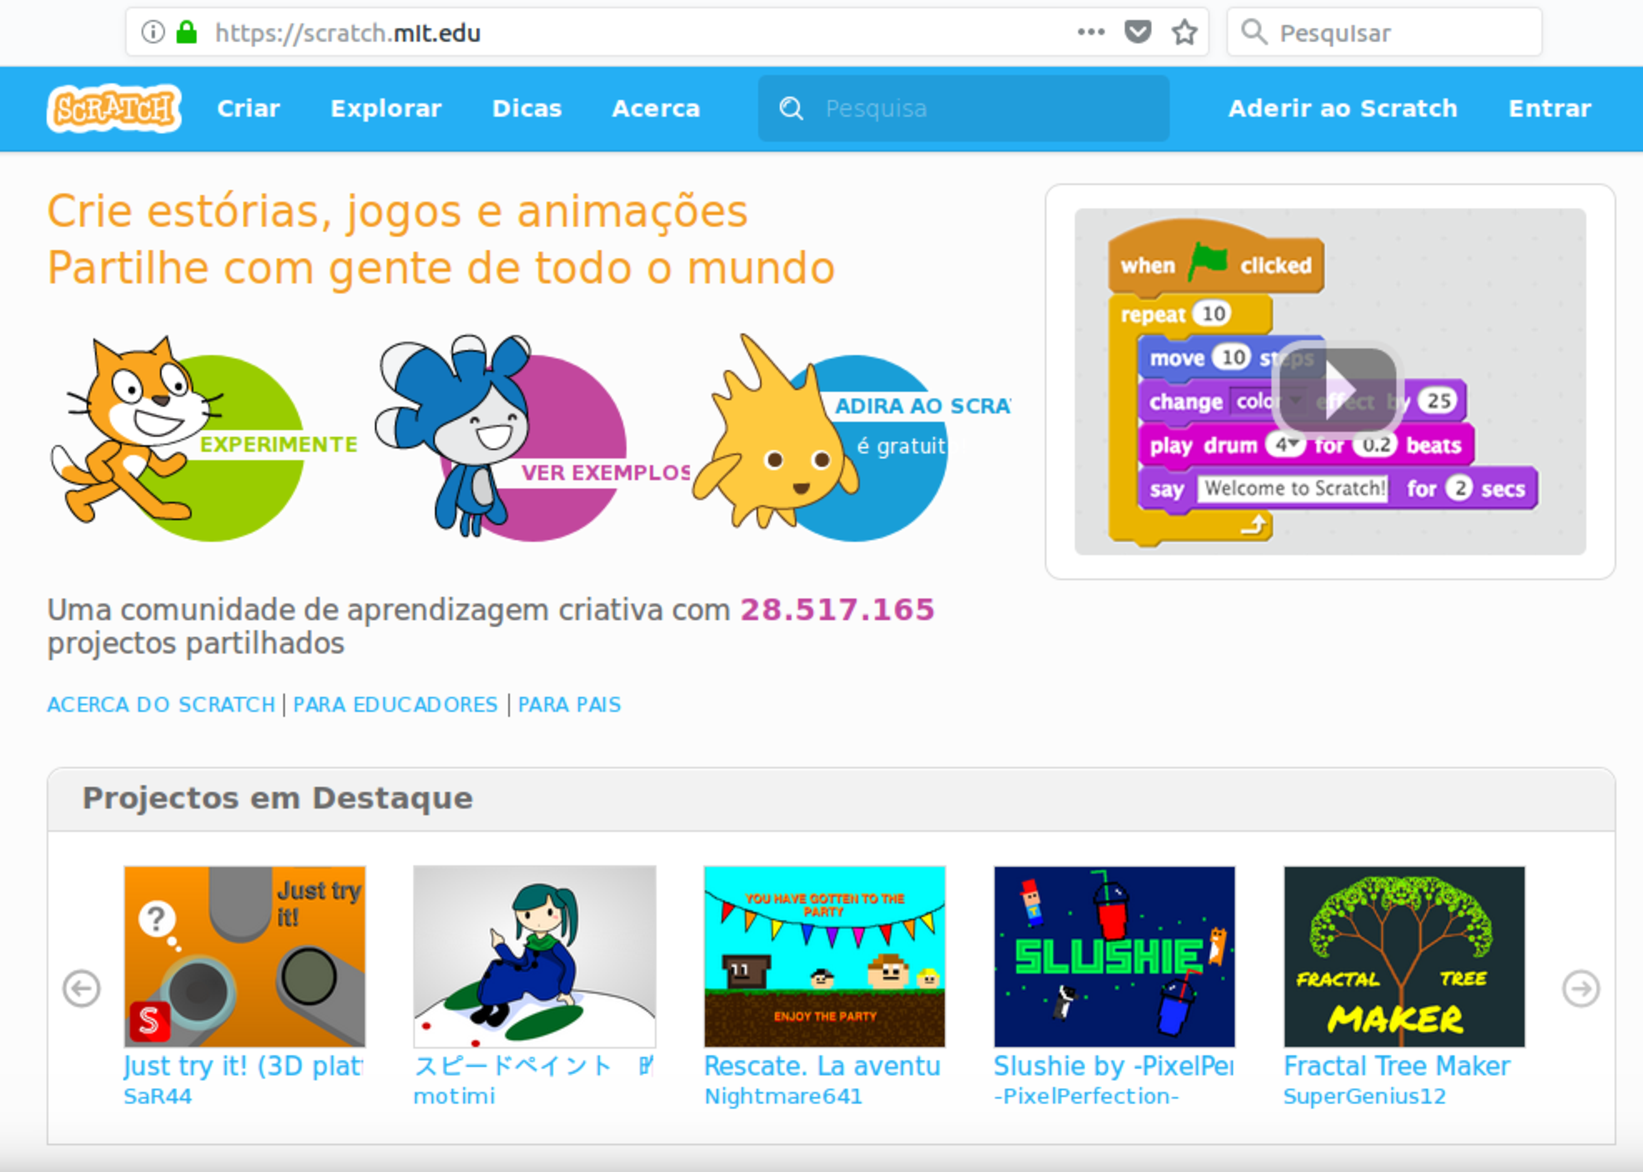
\includegraphics[width=0.7 \textwidth]{Produto/site_scratch}
	\caption{Site \textit{Scratch}}
	\label{fig:app_a:sitescratch}
\end{figure}

\textbf{2º Passo}: Vá até a barra de pesquisa e digite o nome do jogo \aspas{Em Busca do Bóson de Higgs}. 


\begin{figure}[h]
	\centering
	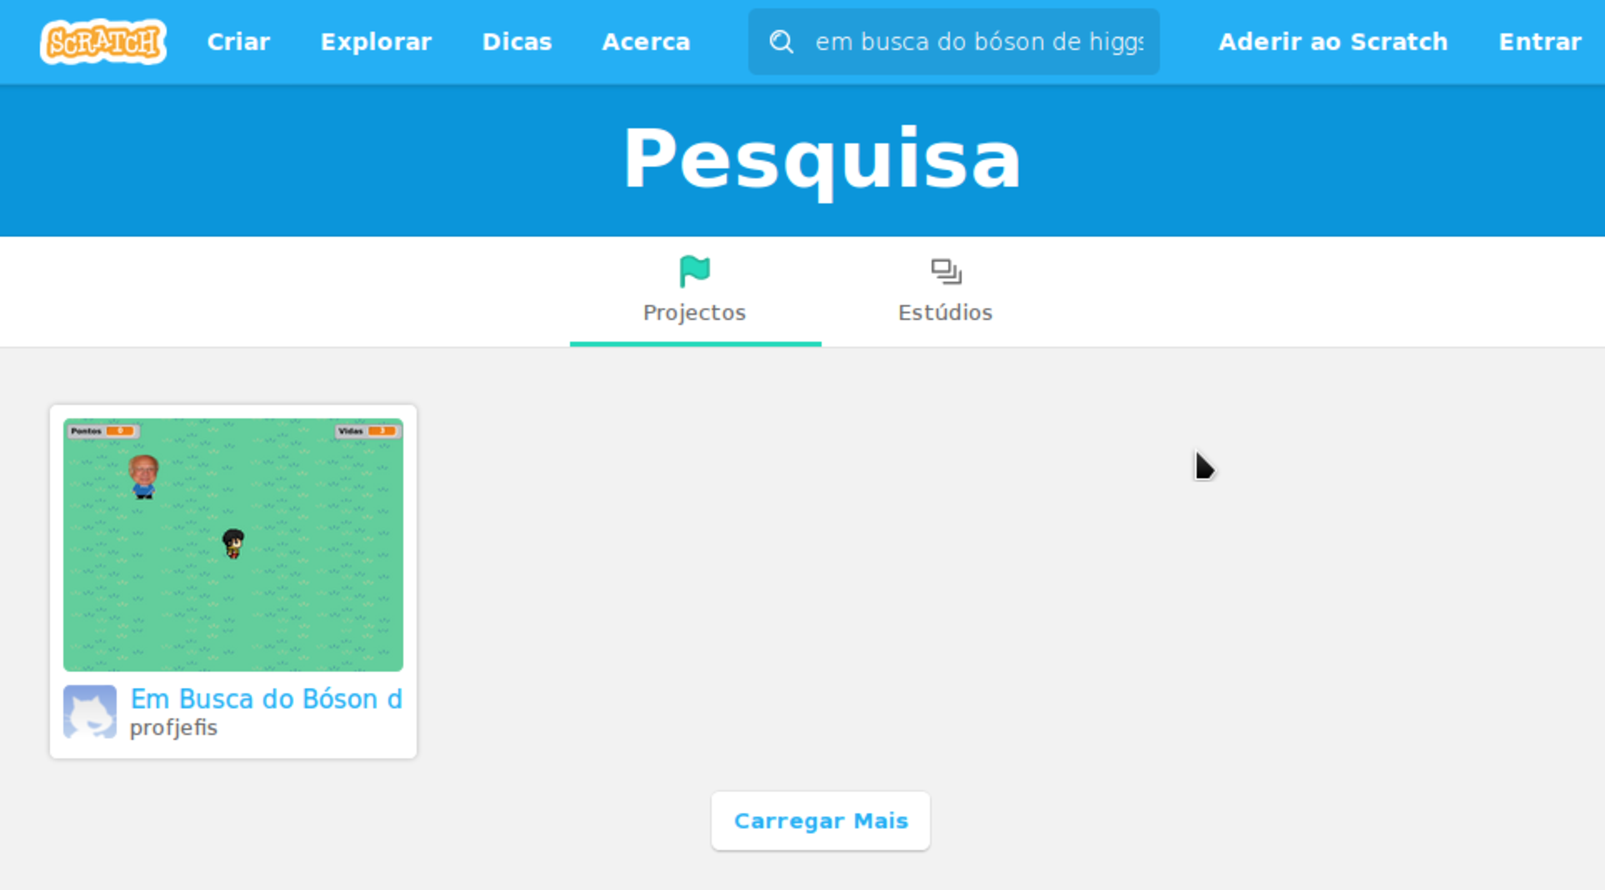
\includegraphics[width=0.7 \textwidth]{Produto/pesquisa}
	\caption{Pesquisa sobre o jogo}
	\label{fig:app_pesquisa}
\end{figure}

\newpage

Clique sobre o projeto que aparece na tela.

\begin{figure}[h]
	\centering
	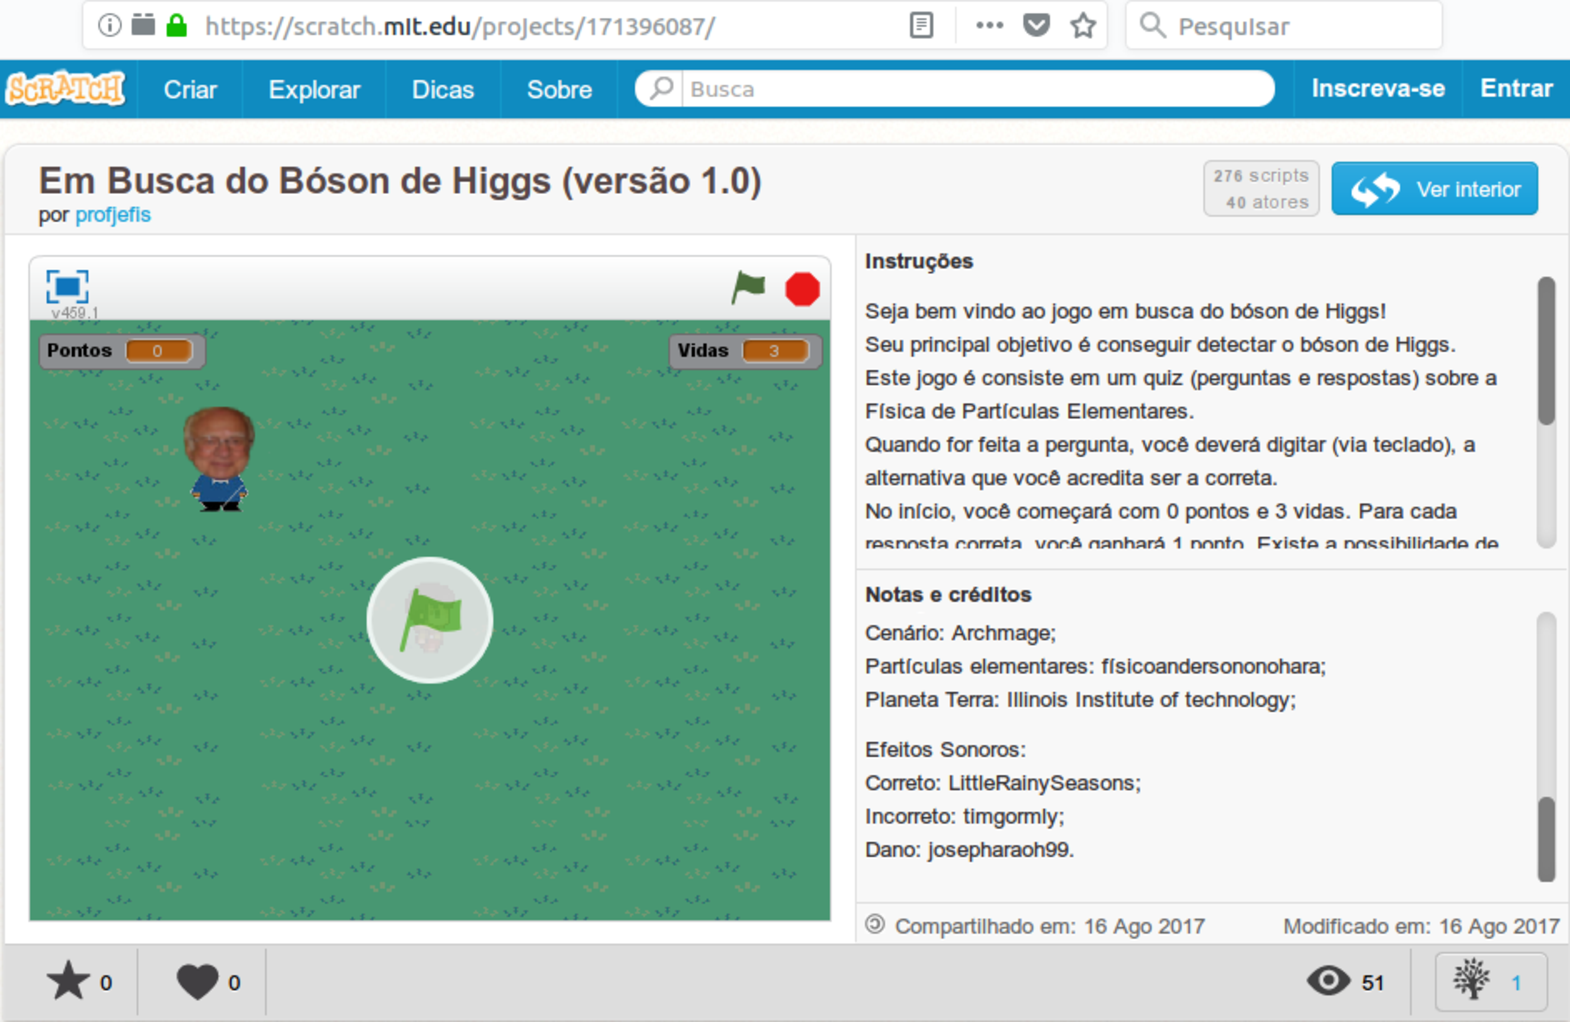
\includegraphics[width=0.7 \textwidth]{Produto/site_jogo}
	\caption{O projeto}
	\label{fig:app_a:projeto}
\end{figure}

\textbf{Forma Direta}:

É possível acessar a mesma tela inicial do jogo acessando diretamente o seguinte \textit{link} \url{https://scratch.mit.edu/projects/171396087/}.

Enfim, ao iniciar o projeto do jogo é necessário clicar no ícone da bandeira verde à direita, enquanto que, para jogar em formato de tela cheia (caso queira), clique no ícone retangular azul à esquerda.

Seguindo estes passos, é possível obter o seguinte resultado:

\begin{figure}[h]
	\centering
	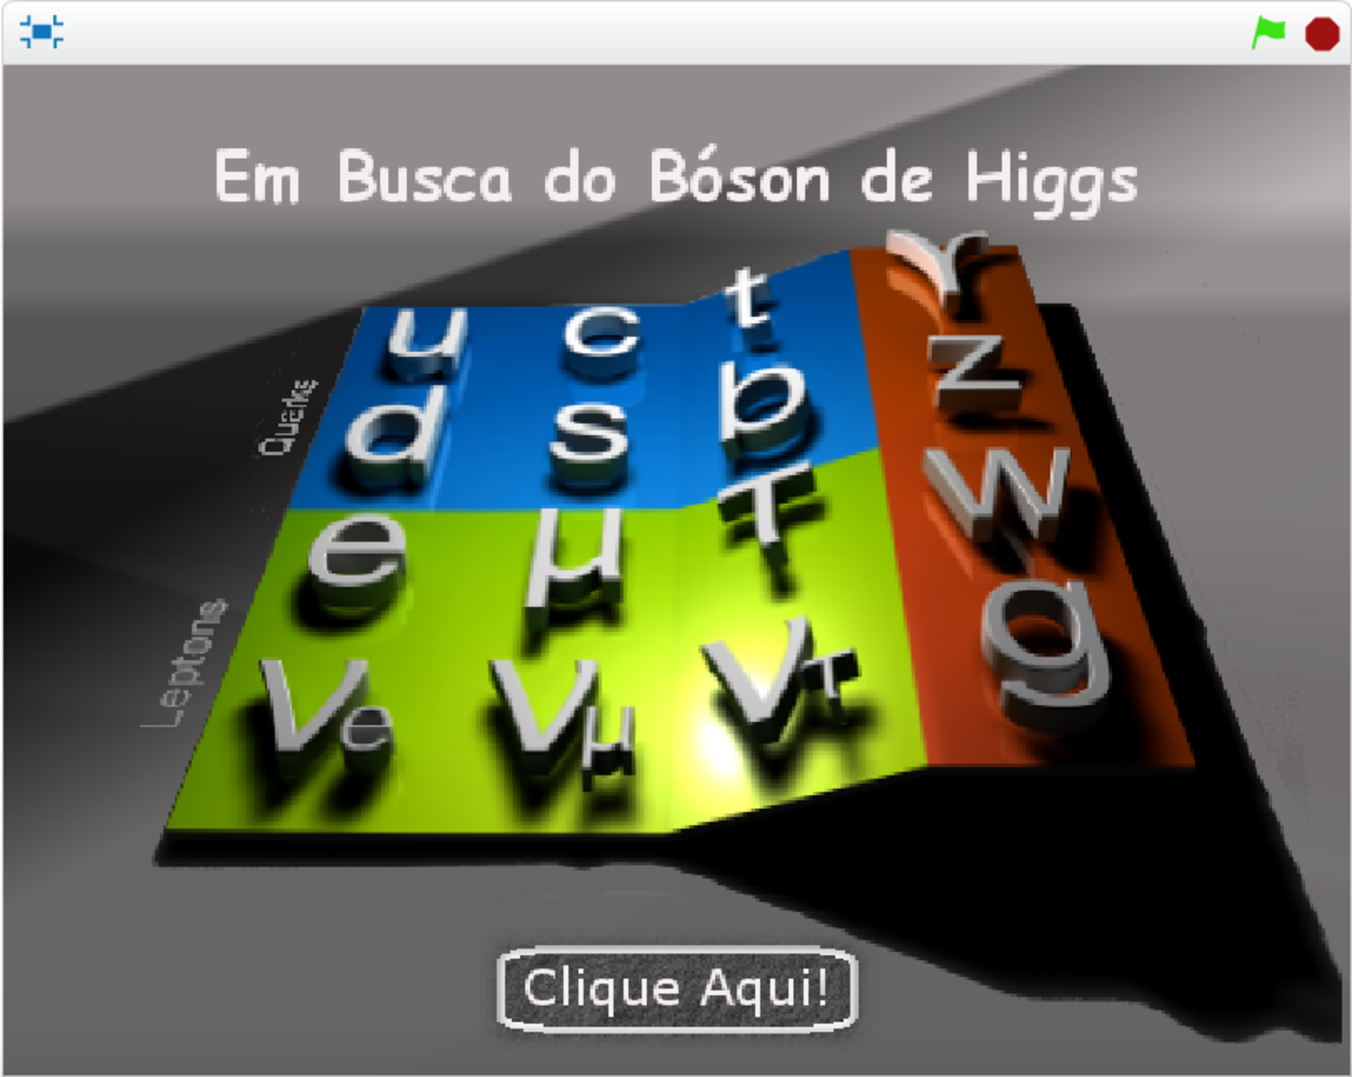
\includegraphics[width=0.65 \textwidth]{Produto/tela_inicial}
	\caption{A tela inicial}
	\label{fig:app_a:telainicial}
\end{figure}

\newpage

Clicando no botão \aspas{Clique Aqui!}, aparecerá a seguinte tela:

\begin{figure}[h]
	\centering
	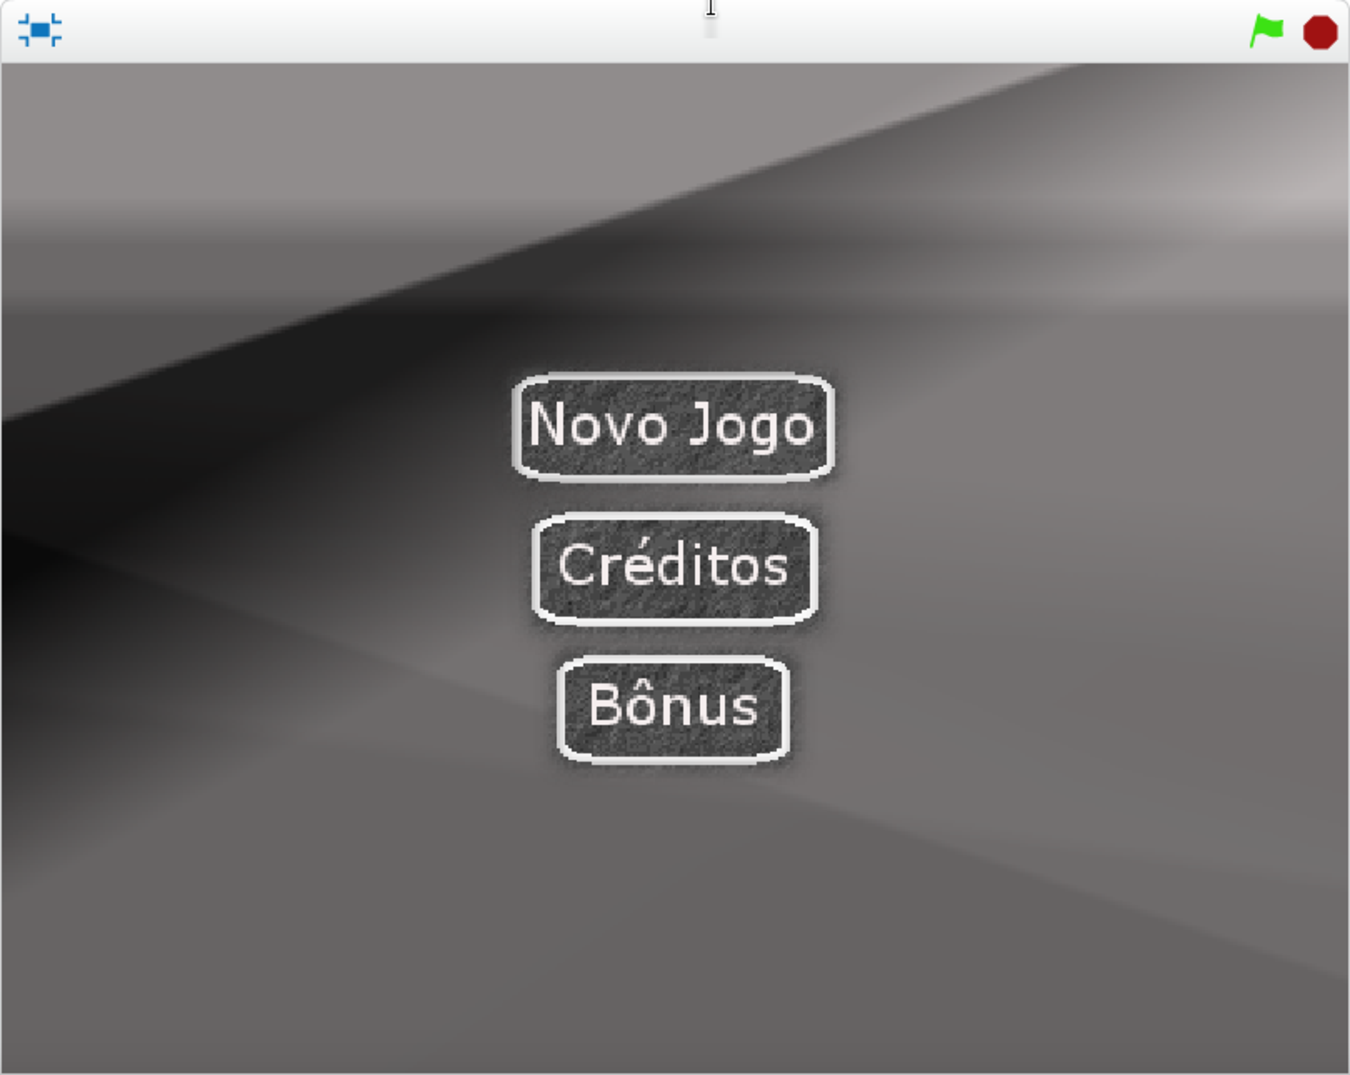
\includegraphics[width=0.65 \textwidth]{Produto/options}
	\caption{Opções}
	\label{fig:app_a:options}
\end{figure}


Antes de comentar sobre o jogo em si, vamos primeiro relatar sobre os créditos e sobre os bônus.

\textbf{Créditos}:

Os créditos retratam toda as referências que utilizamos para elaborar o jogo.

\begin{figure}[h]
	\centering
	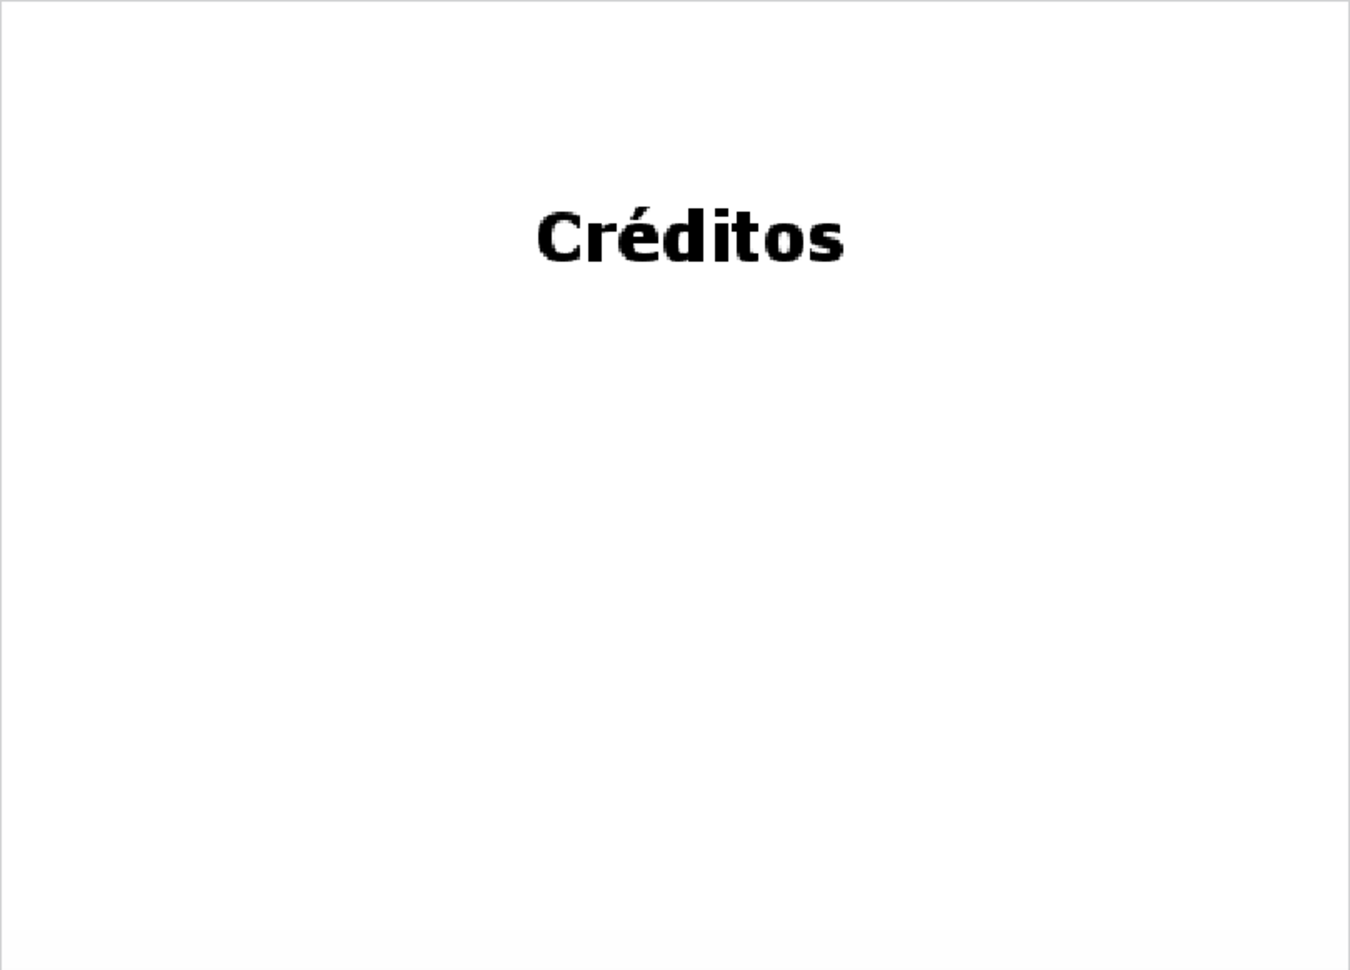
\includegraphics[width=0.65 \textwidth]{Produto/credits}
	\caption{Créditos}
	\label{fig:app_a:credits}
\end{figure}

O créditos estão relacionados com: a programação, o enredo, os \textit{backgrounds} (pano de fundo), os \textit{sprites} (imagens dos personagens, cenários,...) e os efeitos sonoros.

\newpage

\section{Atividades Extras}

Existem dois tipos de bônus (atividades extras):

\begin{figure}[h]
	\centering
	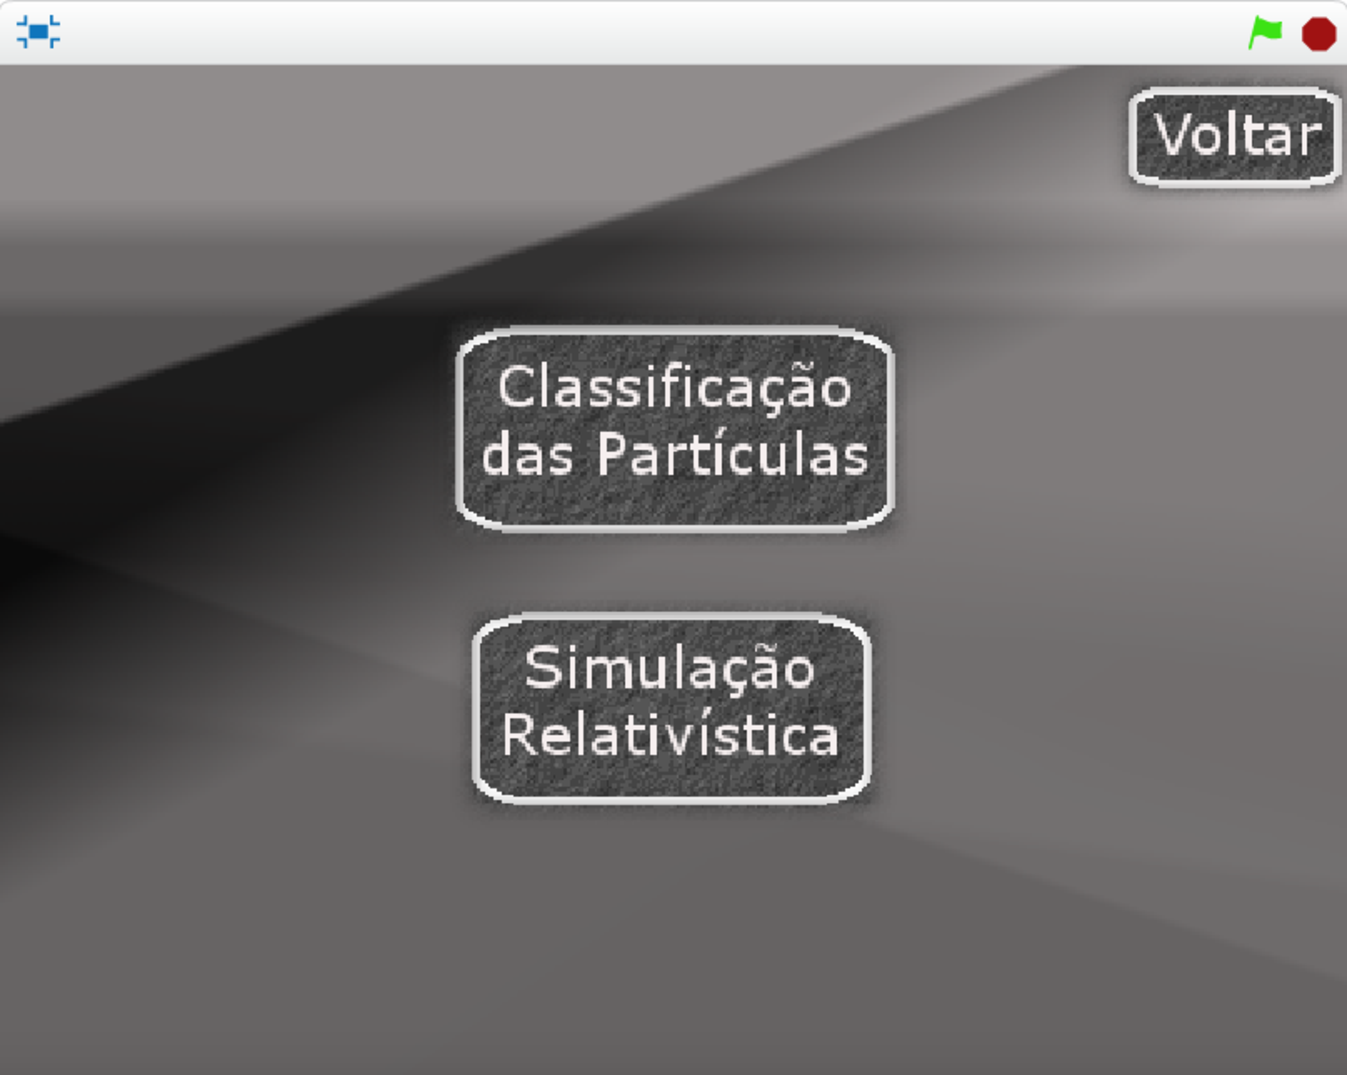
\includegraphics[width=0.65 \textwidth]{Produto/extras}
	\caption{Atividades extras}
	\label{fig:app_a:extras}
\end{figure}


\textbf{Classificação das Partículas}

Clicando no botão \aspas{Classificação das Partículas}, aparecerá uma tela com a explicação da dinâmica do mini game.

\begin{figure}[h]
	\centering
	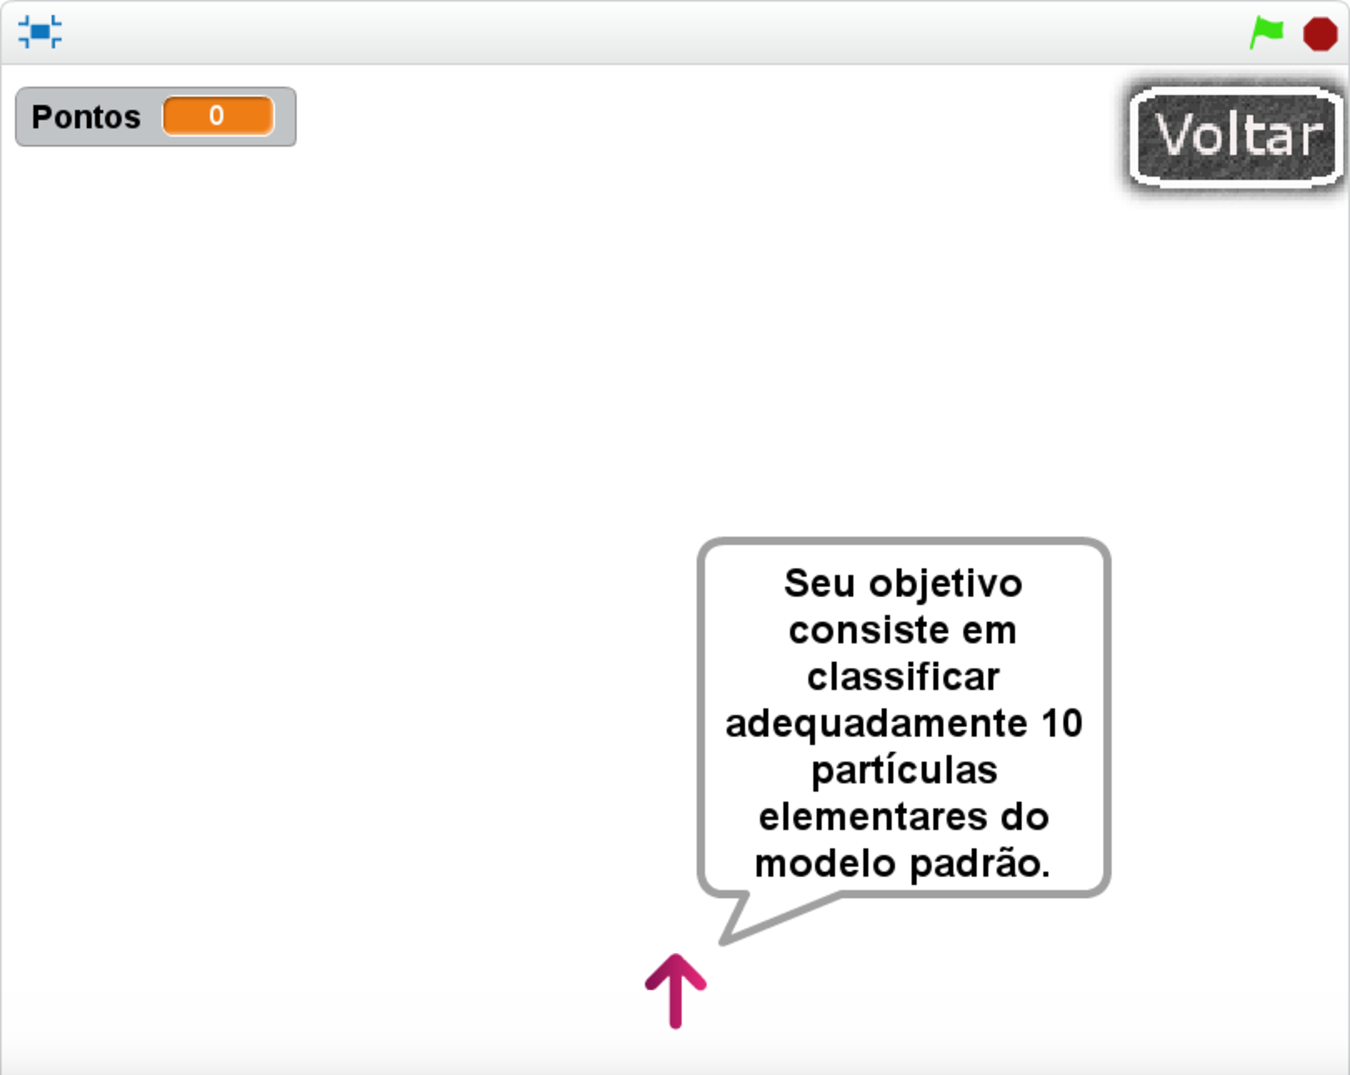
\includegraphics[width=0.65 \textwidth]{Produto/class1}
	\caption{Classificação: tela inicial}
	\label{fig:app_a:class1}
\end{figure}

\newpage

Após a explicação, aparecerá uma tela com a tabela de classificação das partículas elementares do modelo padrão.

\begin{figure}[h]
	\centering
	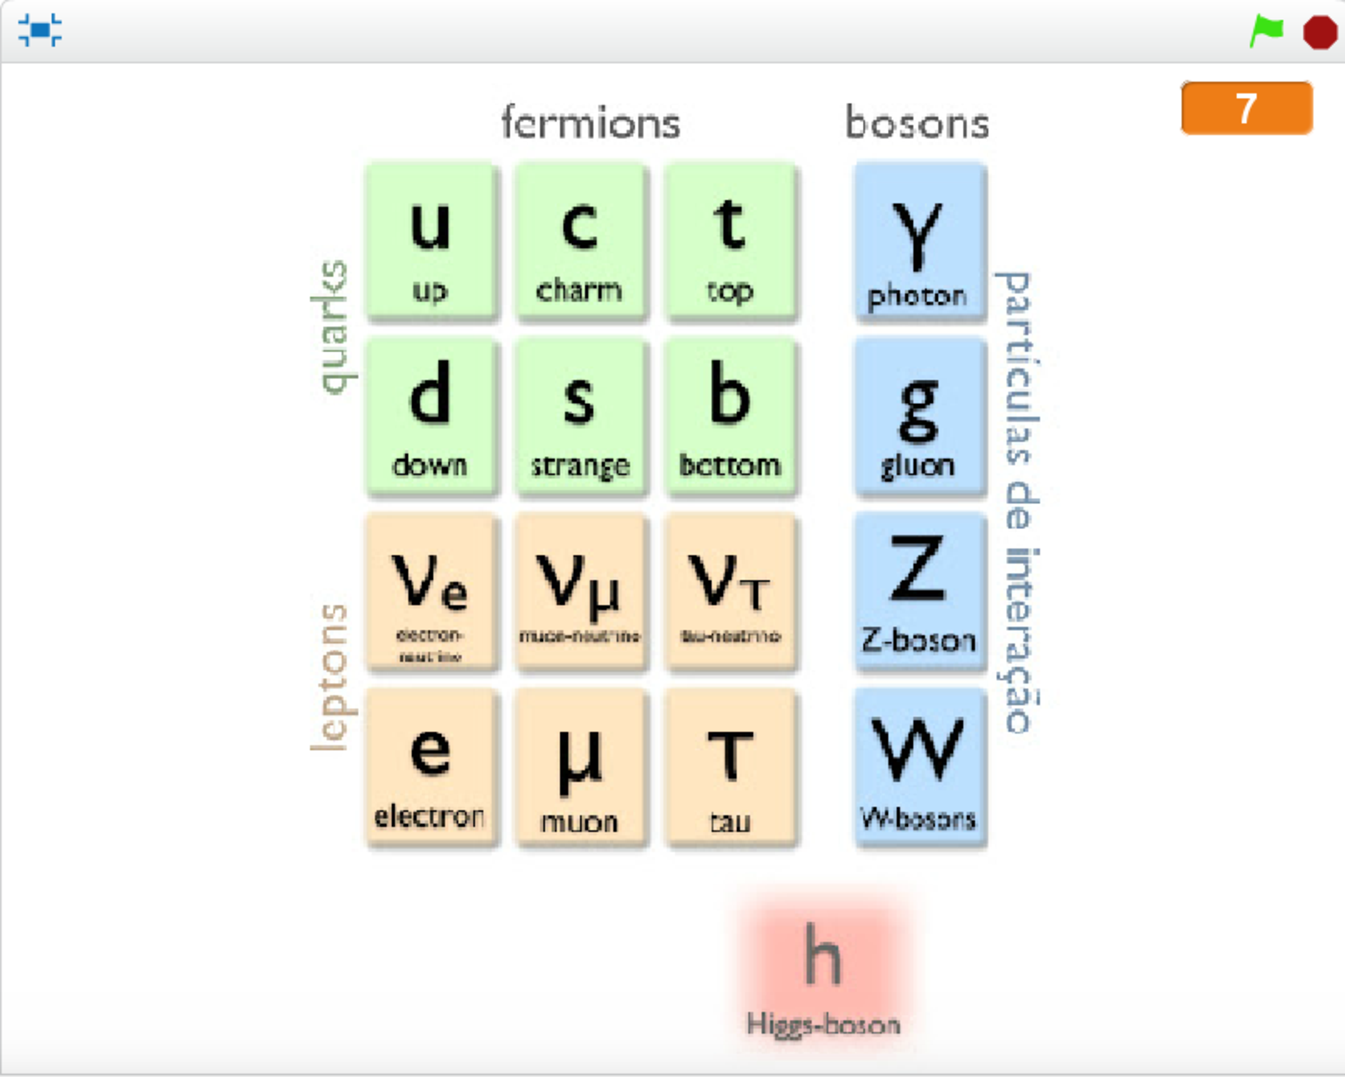
\includegraphics[width=0.65 \textwidth]{Produto/class2}
	\caption{Partículas do modelo padrão}
	\label{fig:app_a:class2}
\end{figure}

No lado direito, aparecerá uma contagem regressiva de 10 segundos. Quando esta contagem chega a 0, a tabela some.

Após esta contagem regressiva, aparecerá uma tela de início da classificação, na parte de baixo uma seta e a partícula a ser classificada e na parte de cima 3 blocos em que as partículas deverão ser classificadas (Quarks, Férmions e Bósons).

\begin{figure}[h]
	\centering
	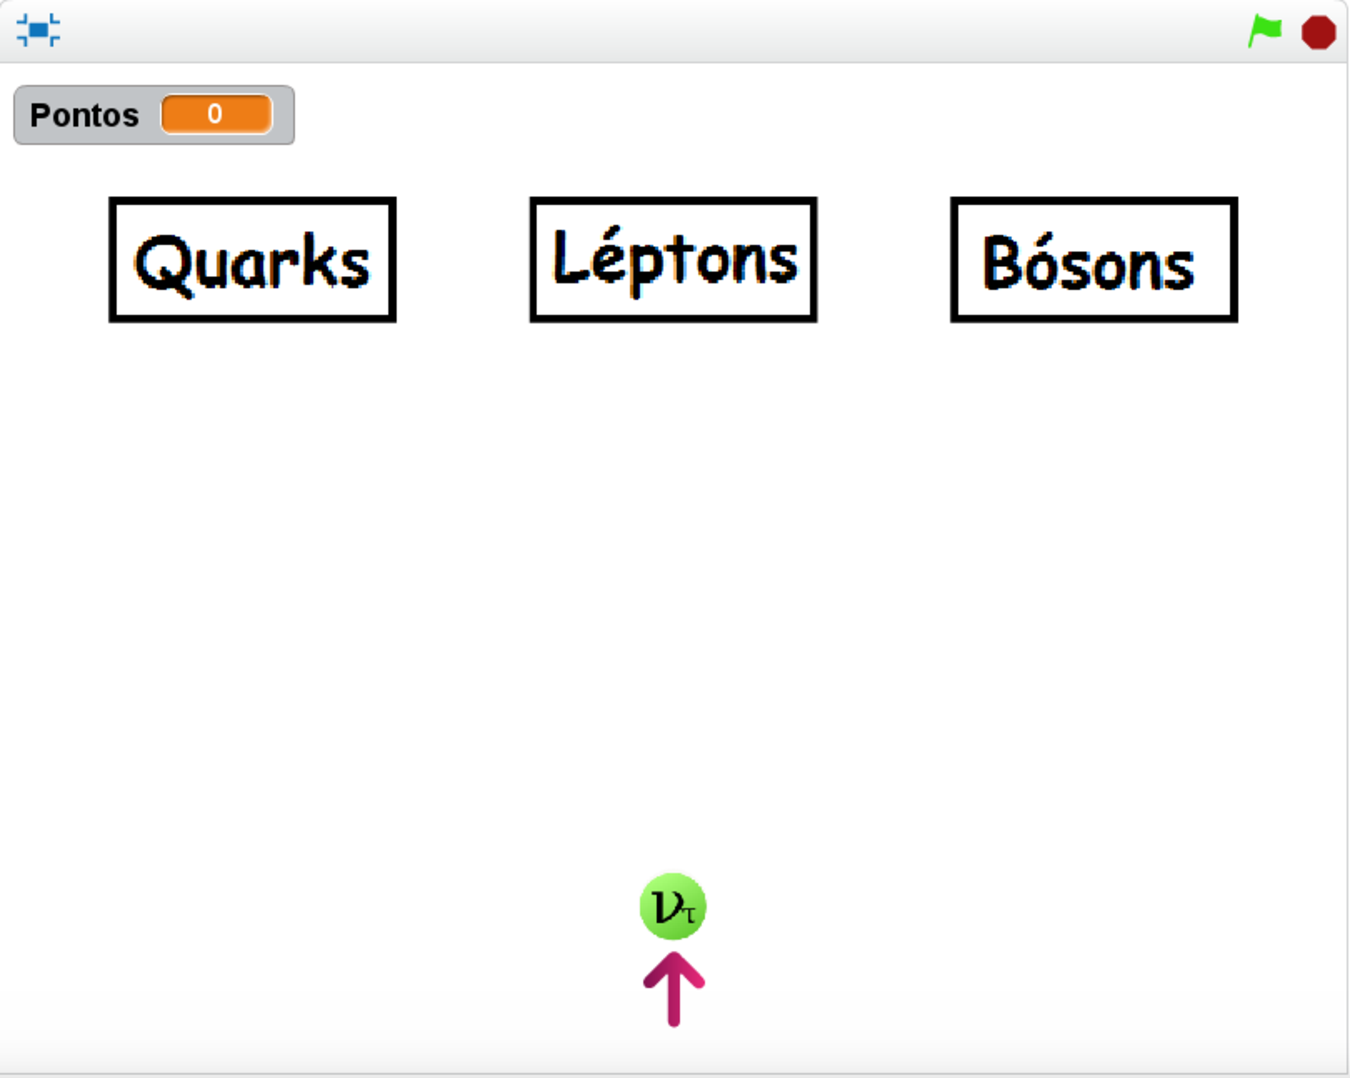
\includegraphics[width=0.63 \textwidth]{Produto/class3}
	\caption{Classe de partículas}
	\label{fig:app_a:class3}
\end{figure}

\newpage

Caso a classificação esteja de acordo com o modelo padrão, a pontuação aumenta em um ponto.

\begin{figure}[h]
	\centering
	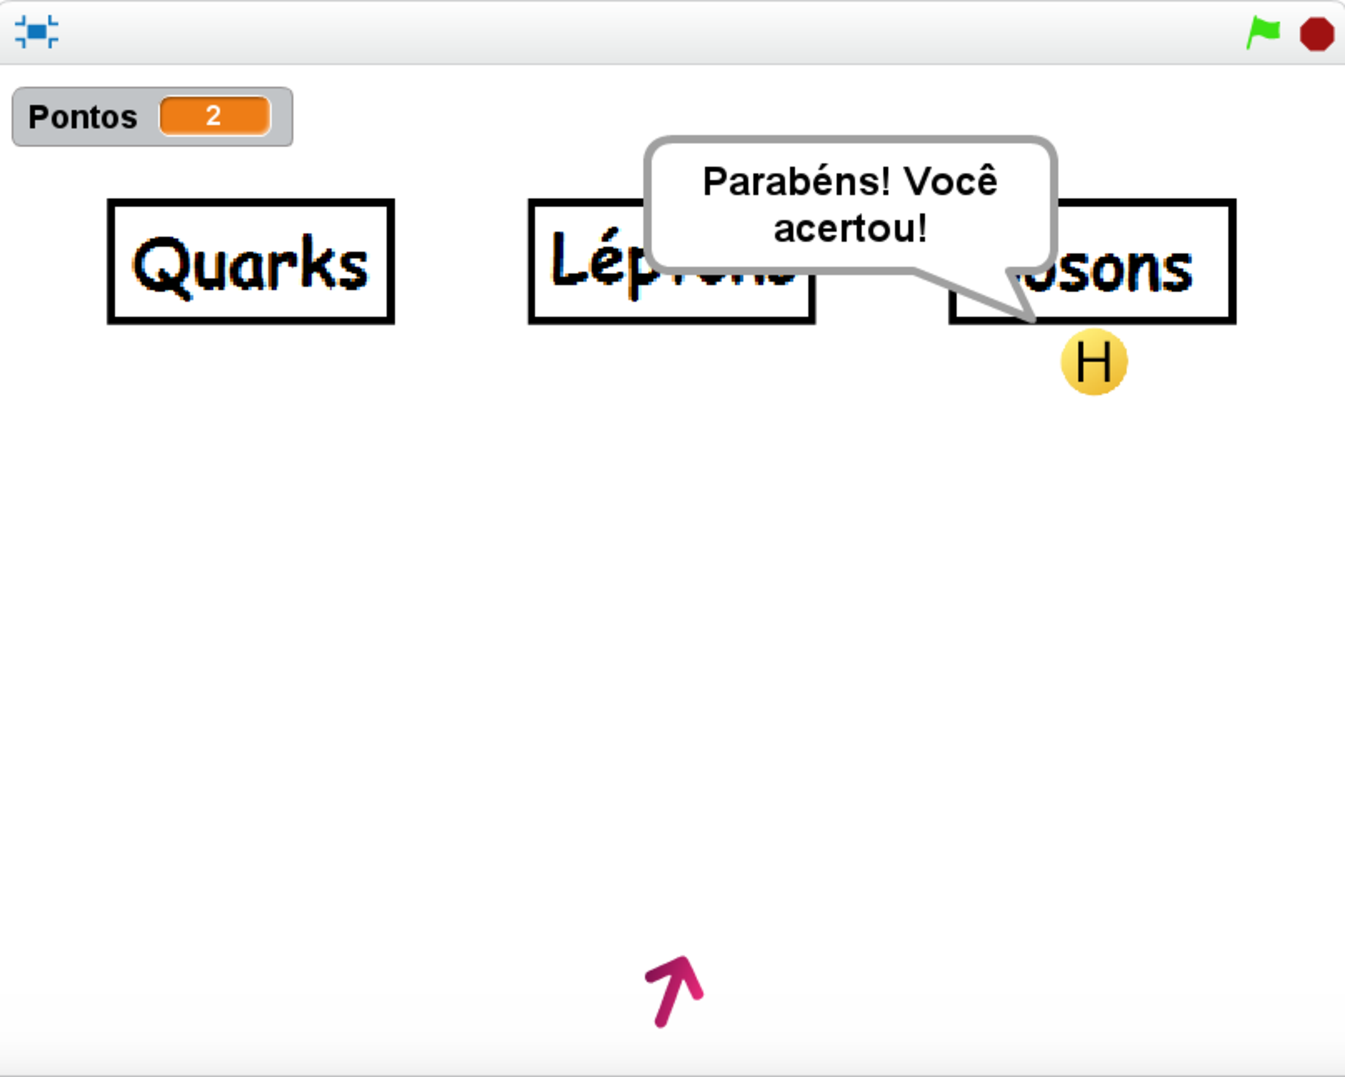
\includegraphics[width=0.65 \textwidth]{Produto/class5}
	\caption{Acertando a classificação}
	\label{fig:app_a:class5}
\end{figure}


O objetivo do mini game é classificar adequadamente 10 partículas elementares do modelo padrão. Caso logre êxito, aparecerá a seguinte tela:

\begin{figure}[h]
	\centering
	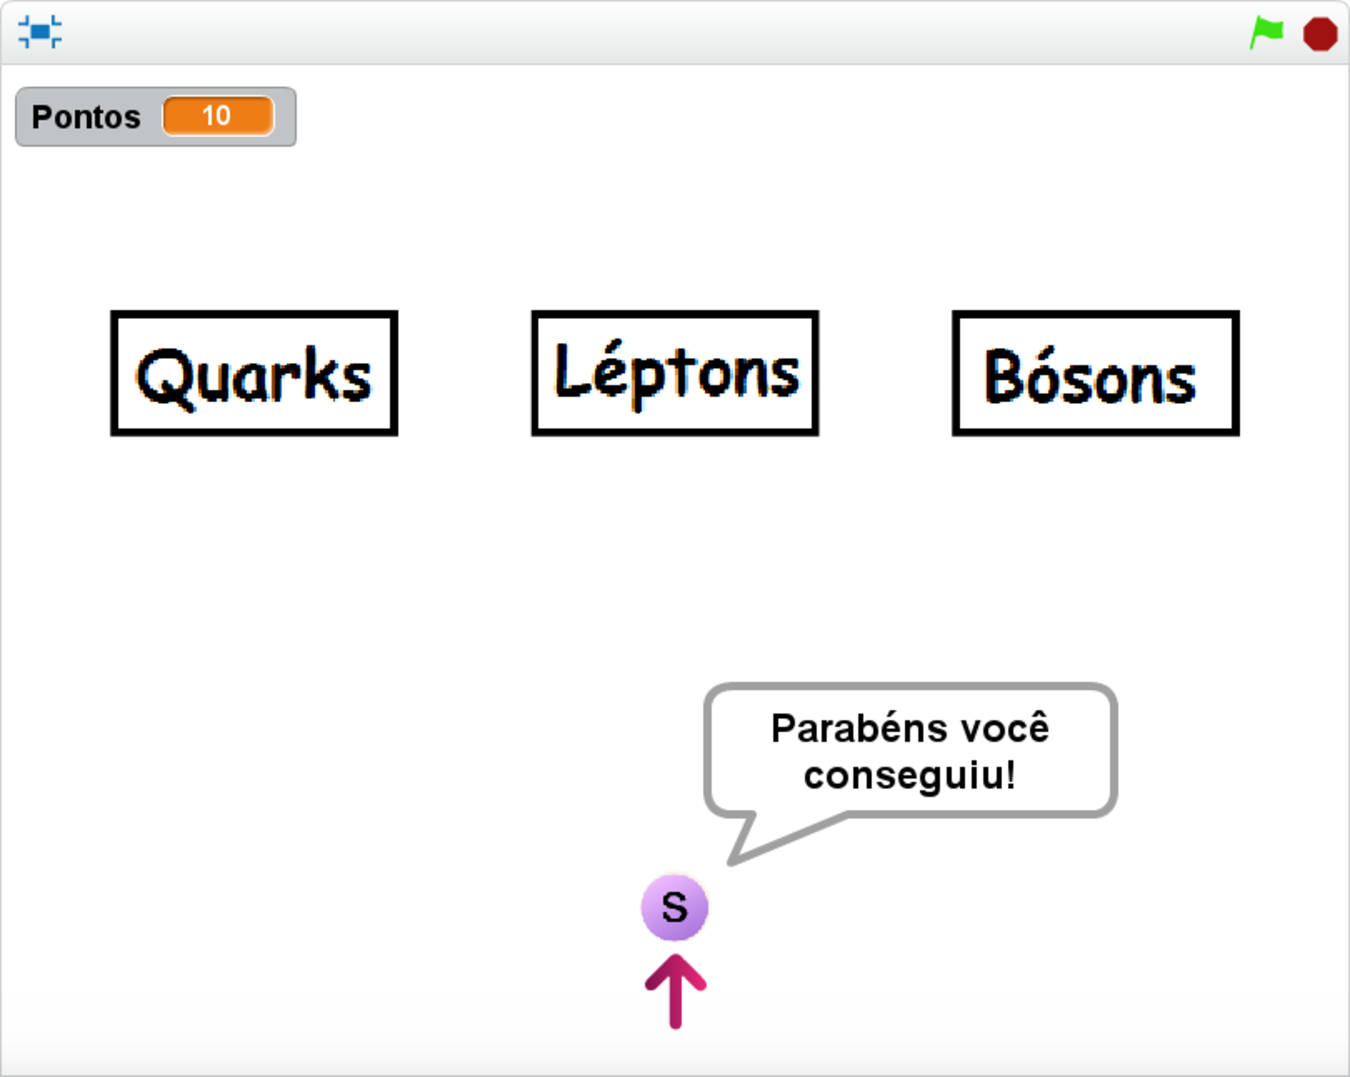
\includegraphics[width=0.63 \textwidth]{Produto/class10}
	\caption{Alcançando o objetivo}
	\label{fig:app_a:class10}
\end{figure}

\newpage

Entretanto, caso a classificação não esteja de acordo com o modelo padrão, os blocos descem...

\begin{figure}[h]
	\centering
	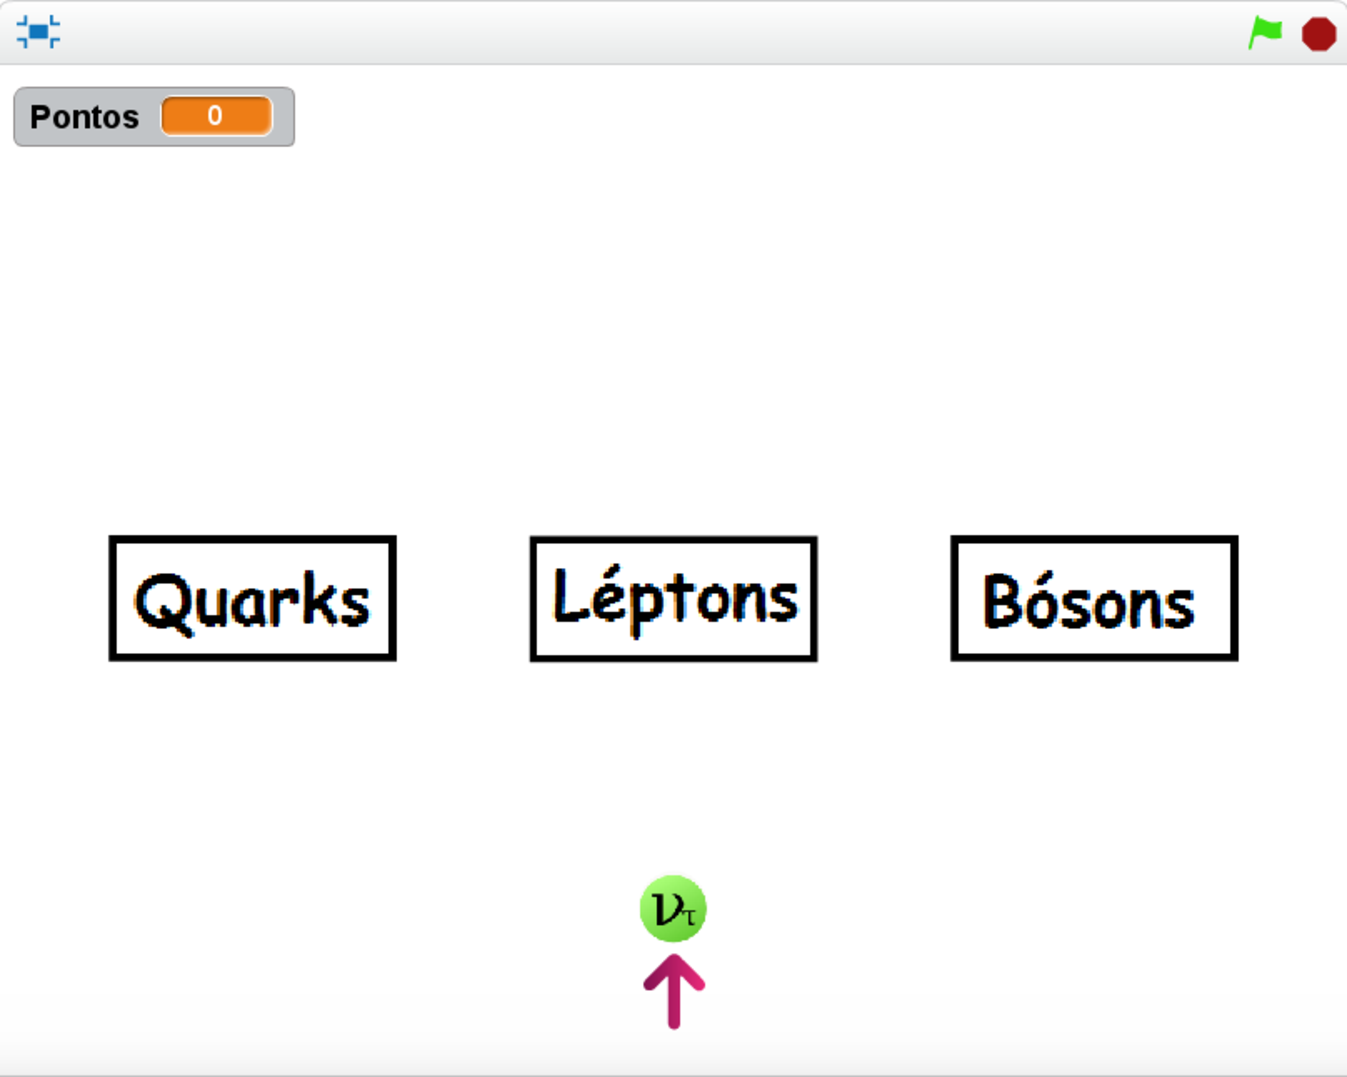
\includegraphics[width=0.65 \textwidth]{Produto/class4}
	\caption{Blocos descendo}
	\label{fig:app_a:class4}
\end{figure}

Caso algum dos blocos colidir com a seta, o jogo terminará:

\begin{figure}[h]
	\centering
	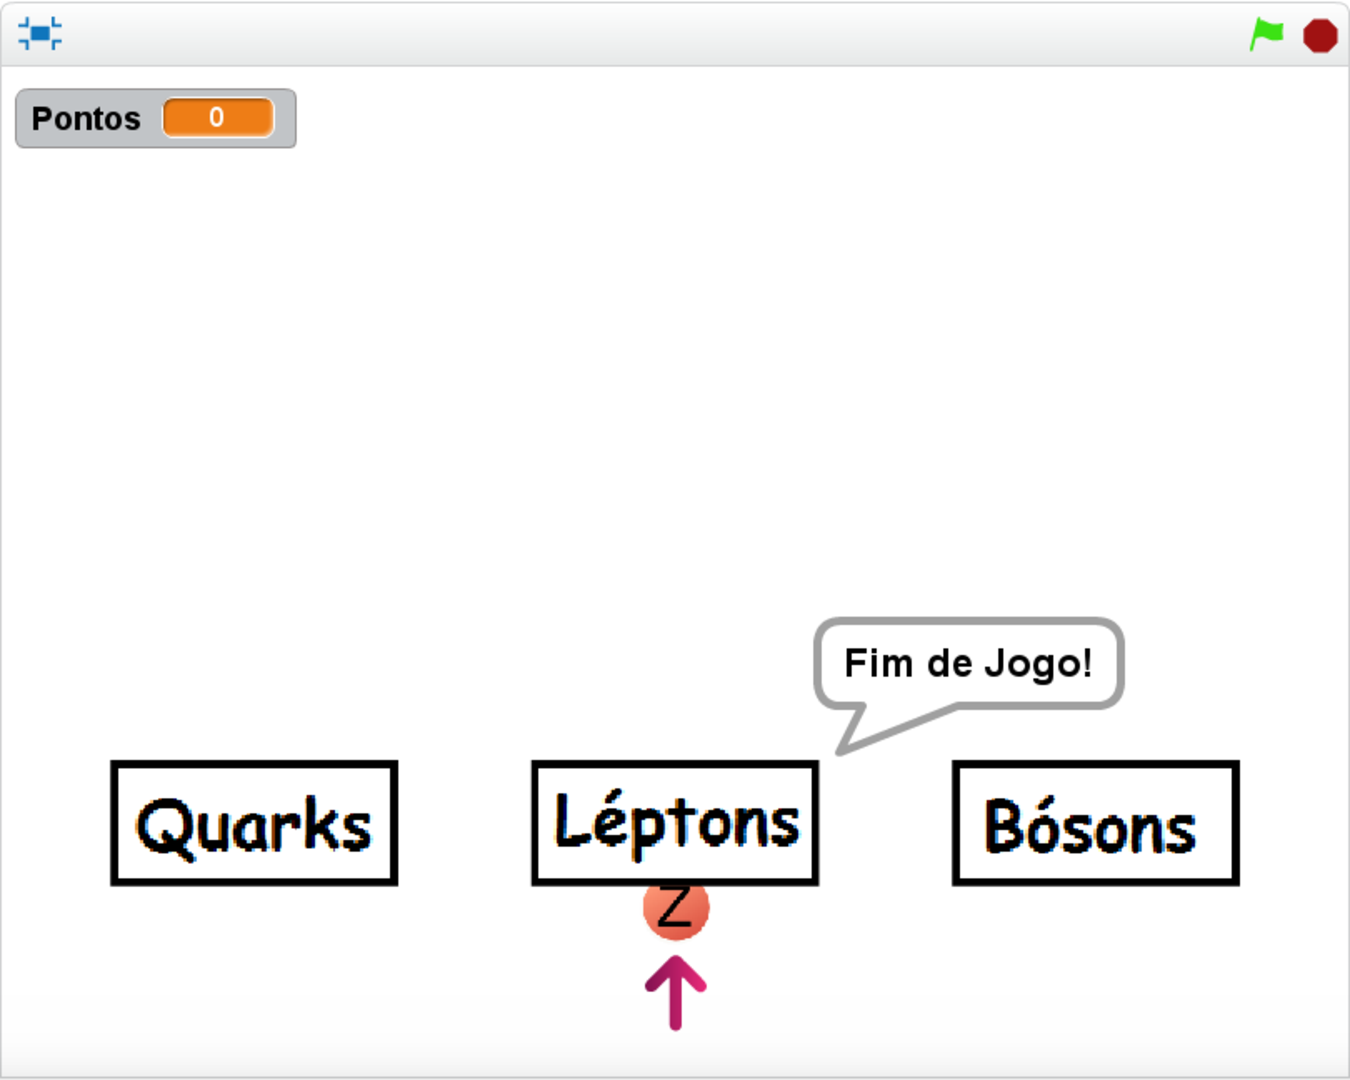
\includegraphics[width=0.63 \textwidth]{Produto/class7}
	\caption{Fim de jogo}
	\label{fig:app_a:class7}
\end{figure}

\newpage

Independente se conseguir alcançar o objetivo ou não, você poderá reiniciar e jogar novamente, quantas vezes desejar.

\begin{figure}[h]
	\centering
	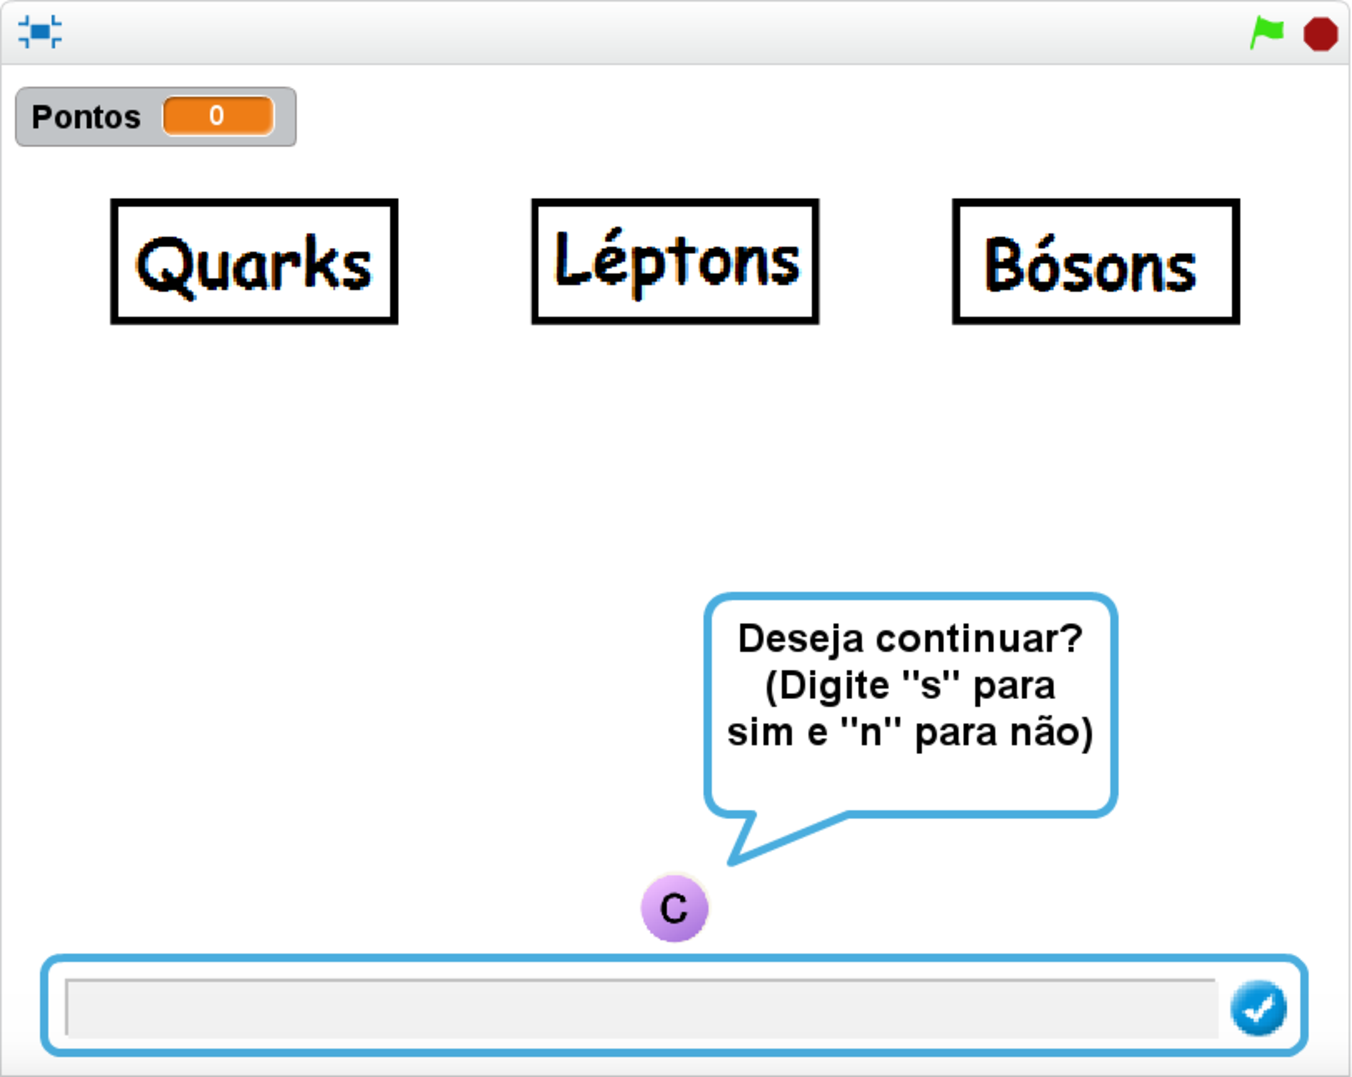
\includegraphics[width=0.65 \textwidth]{Produto/class9}
	\caption{Possível reinício}
	\label{fig:app_a:class9}
\end{figure}

Mesmo que este mini game esteja relacionado com conhecimentos memorísticos e que tenha traços de aprendizagem mecânica, ele tem como objetivo não apenas a \aspas{decoreba} por si mesmo, mas sim, uma ambientação dos termos mais complexos da FPE.

\textbf{Simulação relativística}

Esta simulação de relatividade restrita tem como objetivo ilustrar o efeito relativístico de dilatação do tempo da partícula denominada: múon.

\begin{figure}[h]
	\centering
	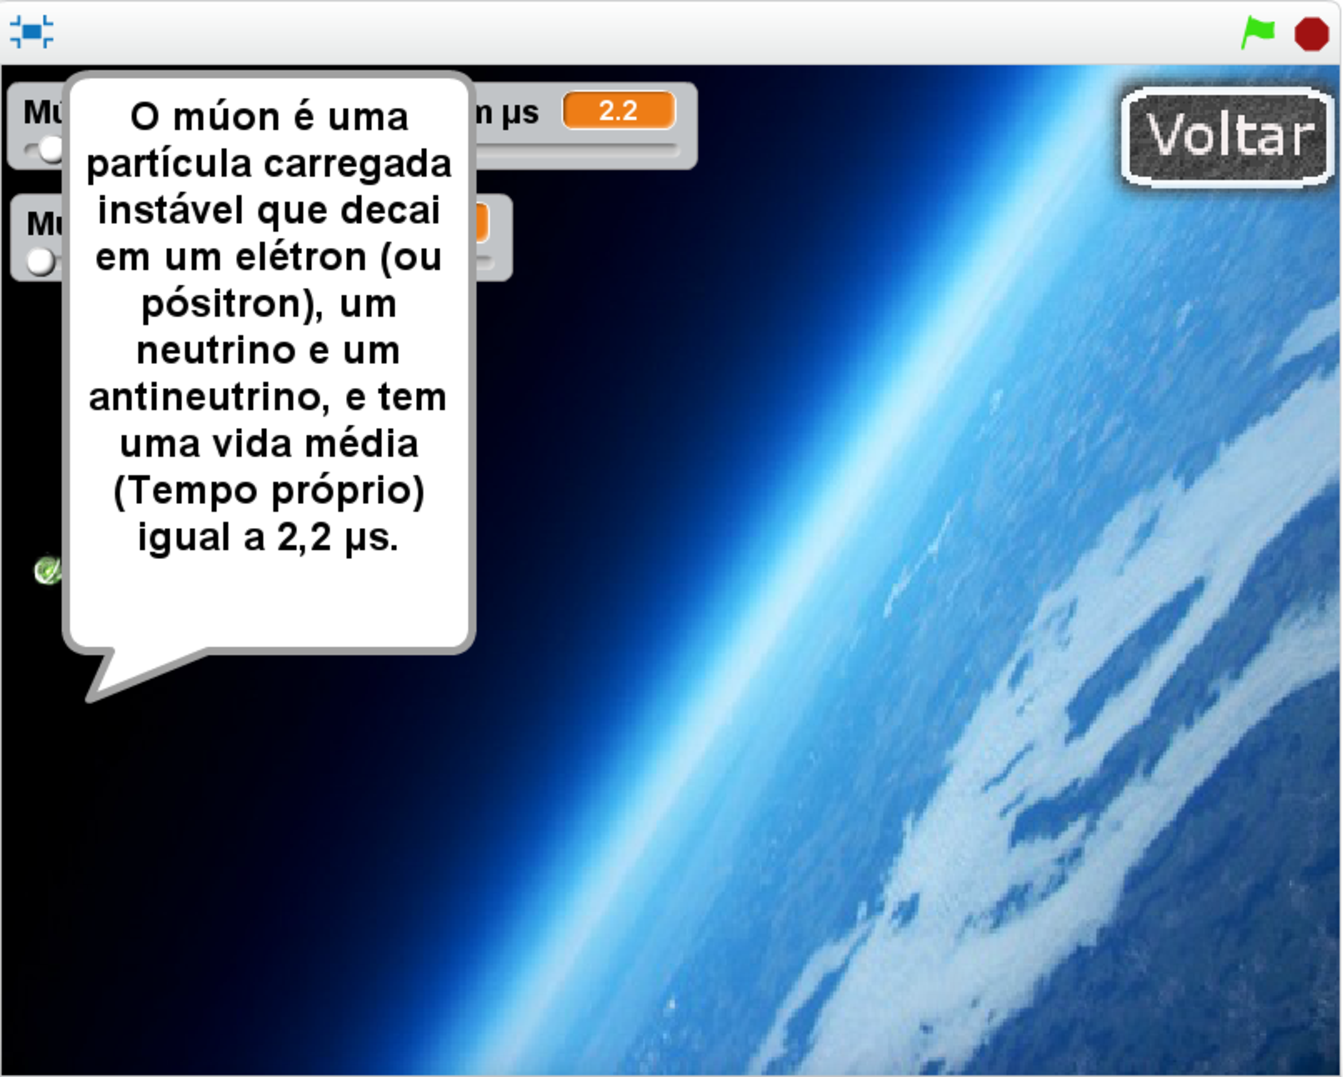
\includegraphics[width=0.6 \textwidth]{Produto/sim1}
	\caption{Explicação da simulação}
	\label{fig:app_a:sim1}
\end{figure}

A principal ideia desta simulação consiste em controlar o parâmetro velocidade do múon e verificar o que acontece com o tempo de vida médio medido no laboratório.

\begin{figure}[h]
	\centering
	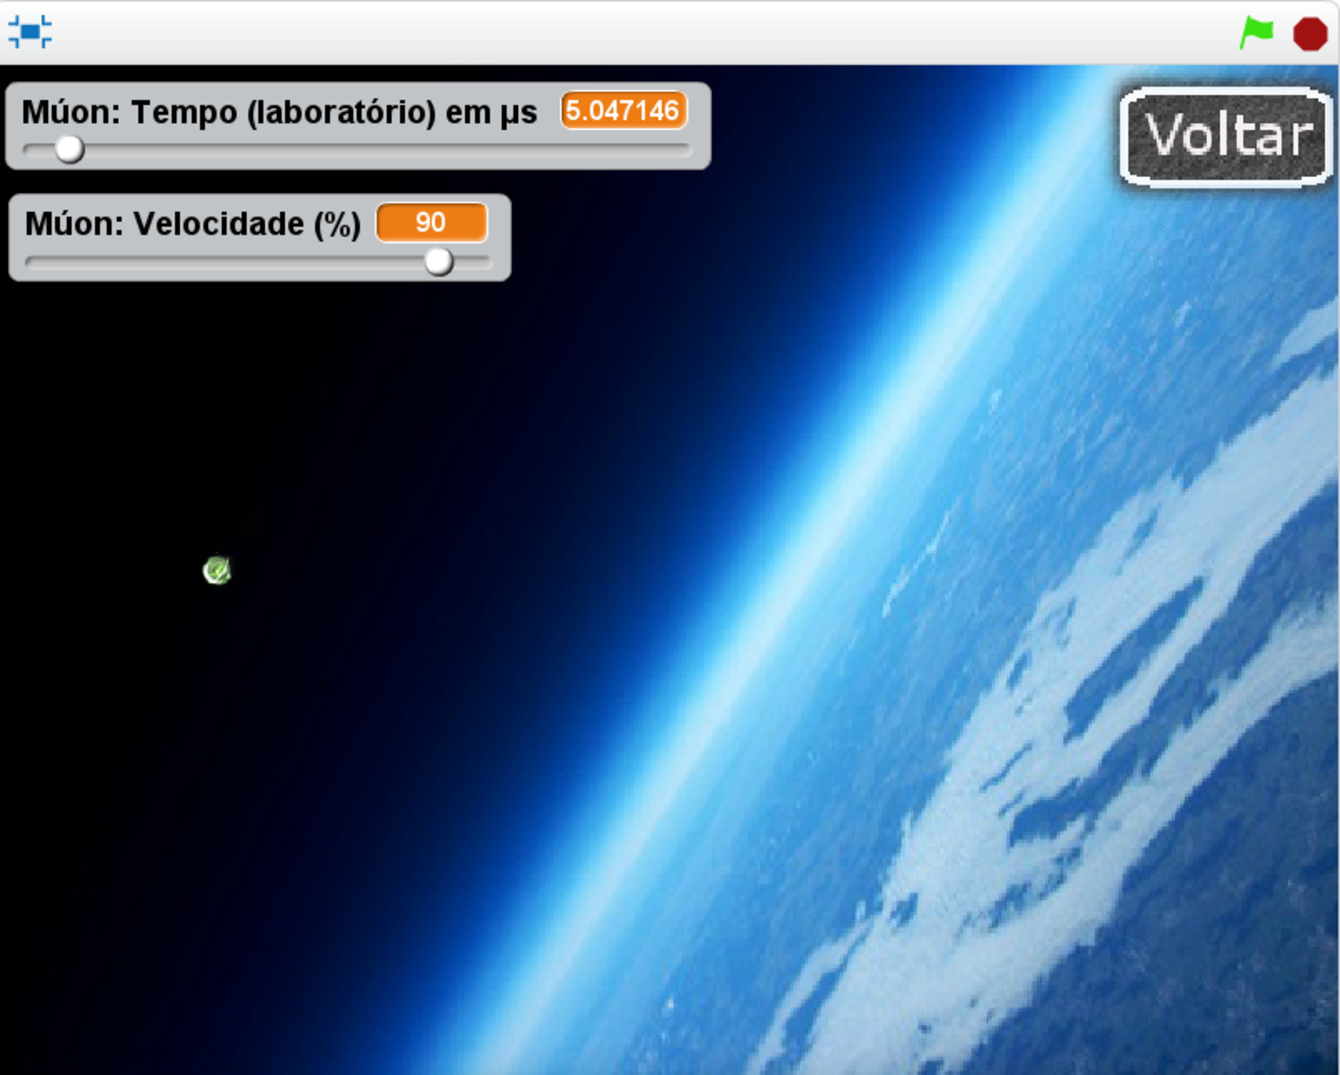
\includegraphics[width=0.6 \textwidth]{Produto/sim2}
	\caption{A simulação}
	\label{fig:app_a:sim2}
\end{figure}


\section{O Jogo Principal}
O jogo \aspas{Em busca do Bóson de Higgs}

Você inicia o jogo no lado norte do mapa, logo abaixo de uma casa. 

\begin{figure}[h]
	\centering
	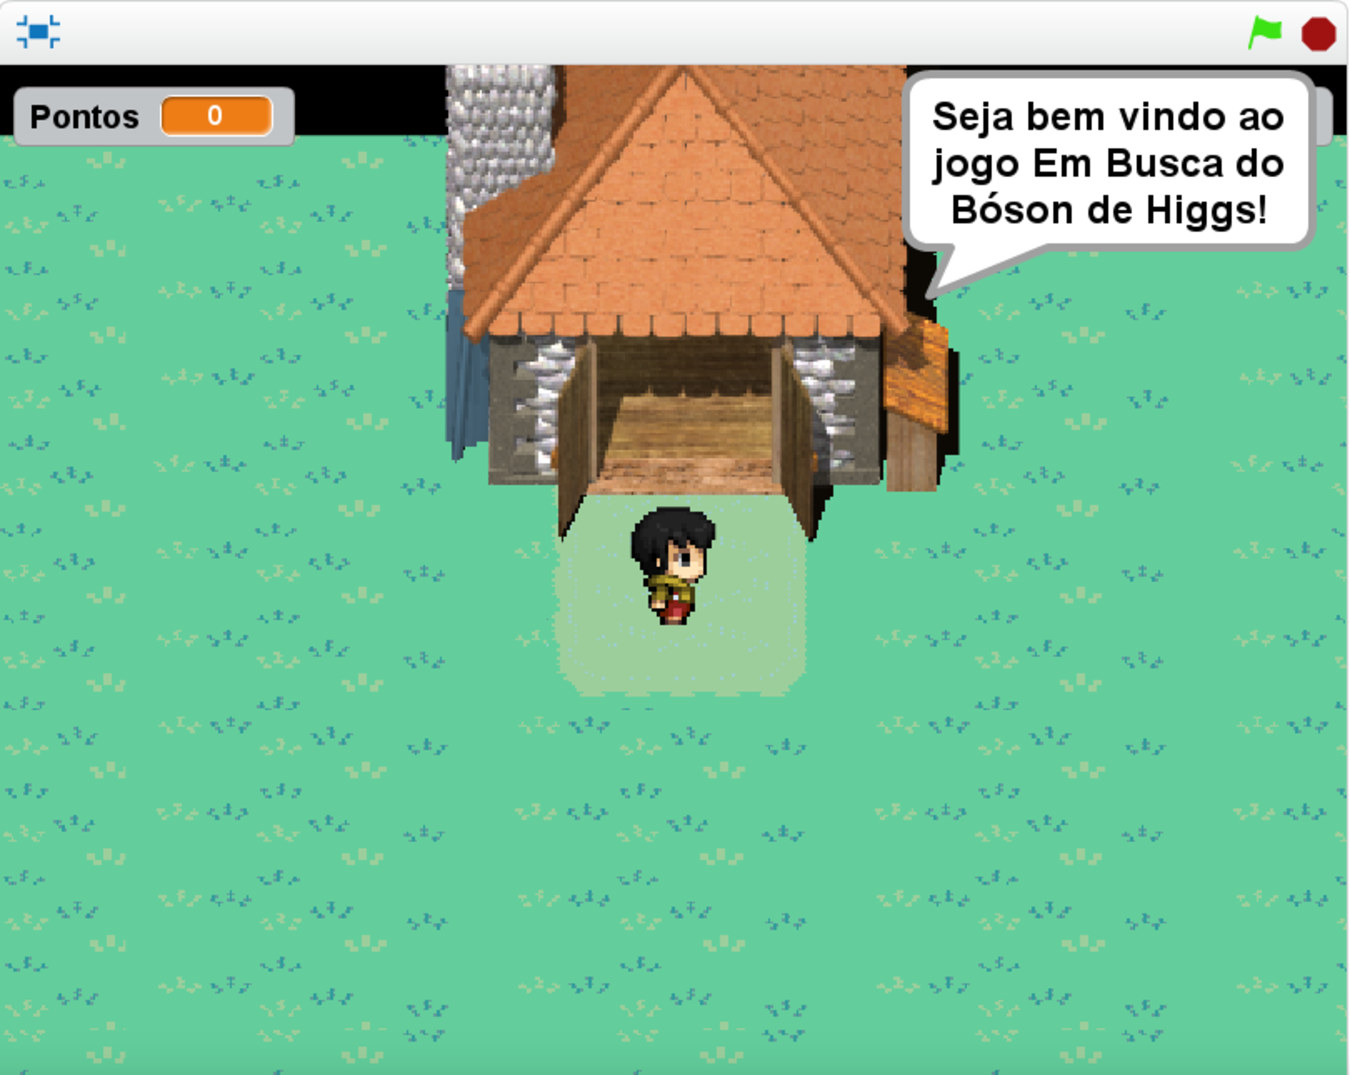
\includegraphics[width=0.65 \textwidth]{Produto/jogo_1}
	\caption{Início do jogo}
	\label{fig:app_a:jogo1}
\end{figure}

\newpage

Aparecerá algumas instruções, você deverá permanecer parado no intuito de ler as instruções. Apenas quando as instruções forem concluídas, você poderá desbravar o mapa da cidade. 

\begin{figure}[h]
	\centering
	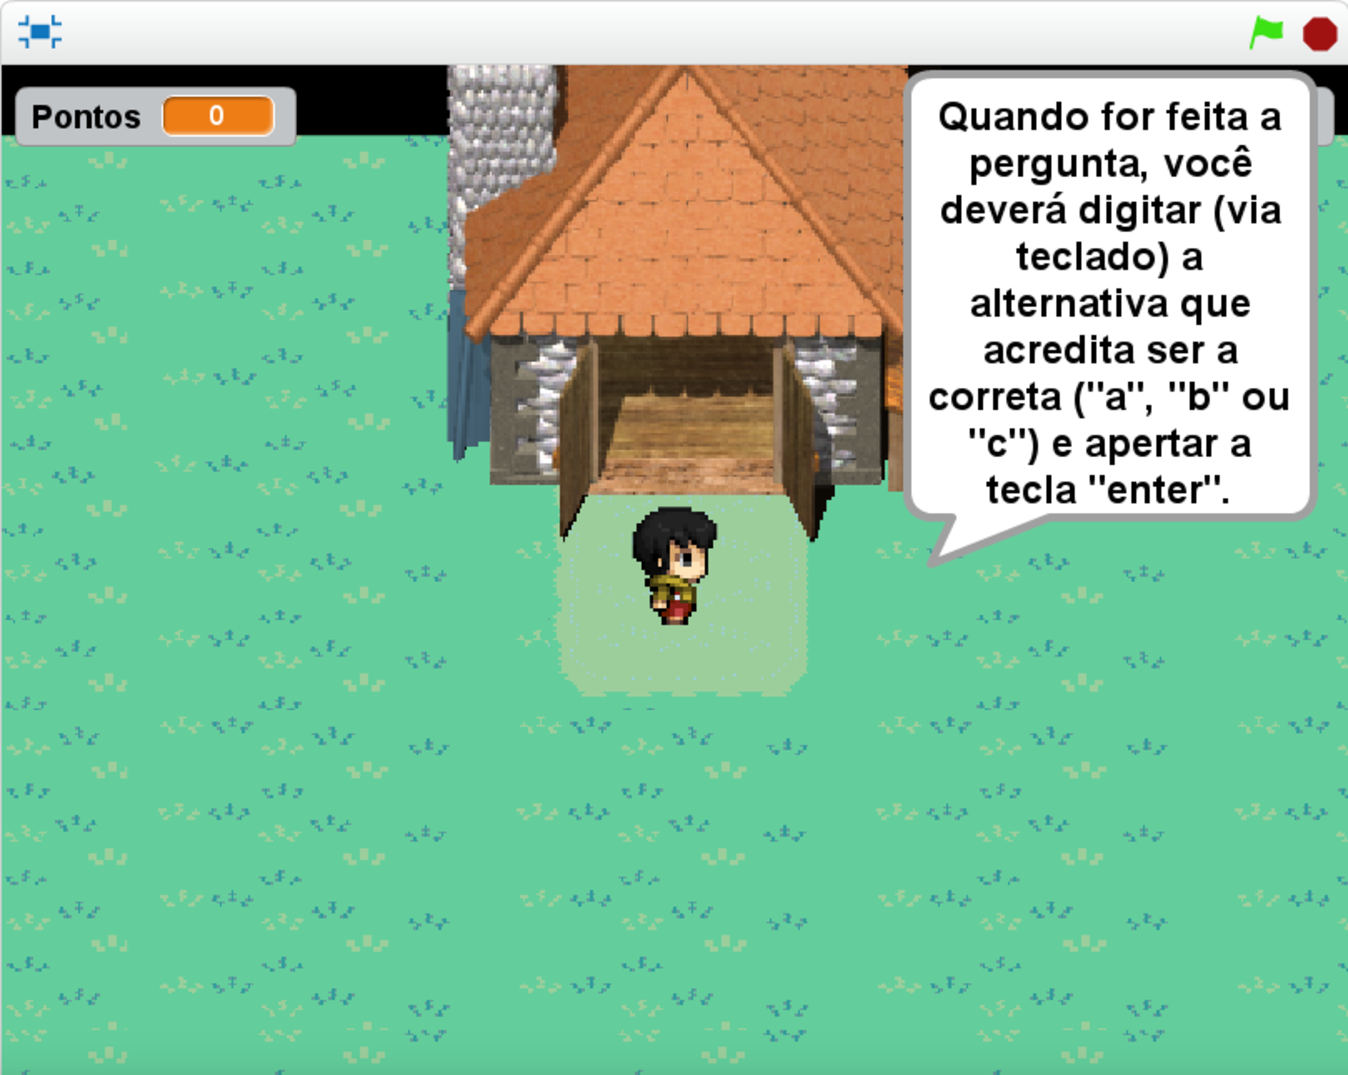
\includegraphics[width=0.65 \textwidth]{Produto/jogo_2}
	\caption{Instruções inicias}
	\label{fig:app_a:jogo2}
\end{figure}

Após as instruções, procure um dos principais personagens da narrativa, Peter Higgs.

\begin{figure}[h]
	\centering
	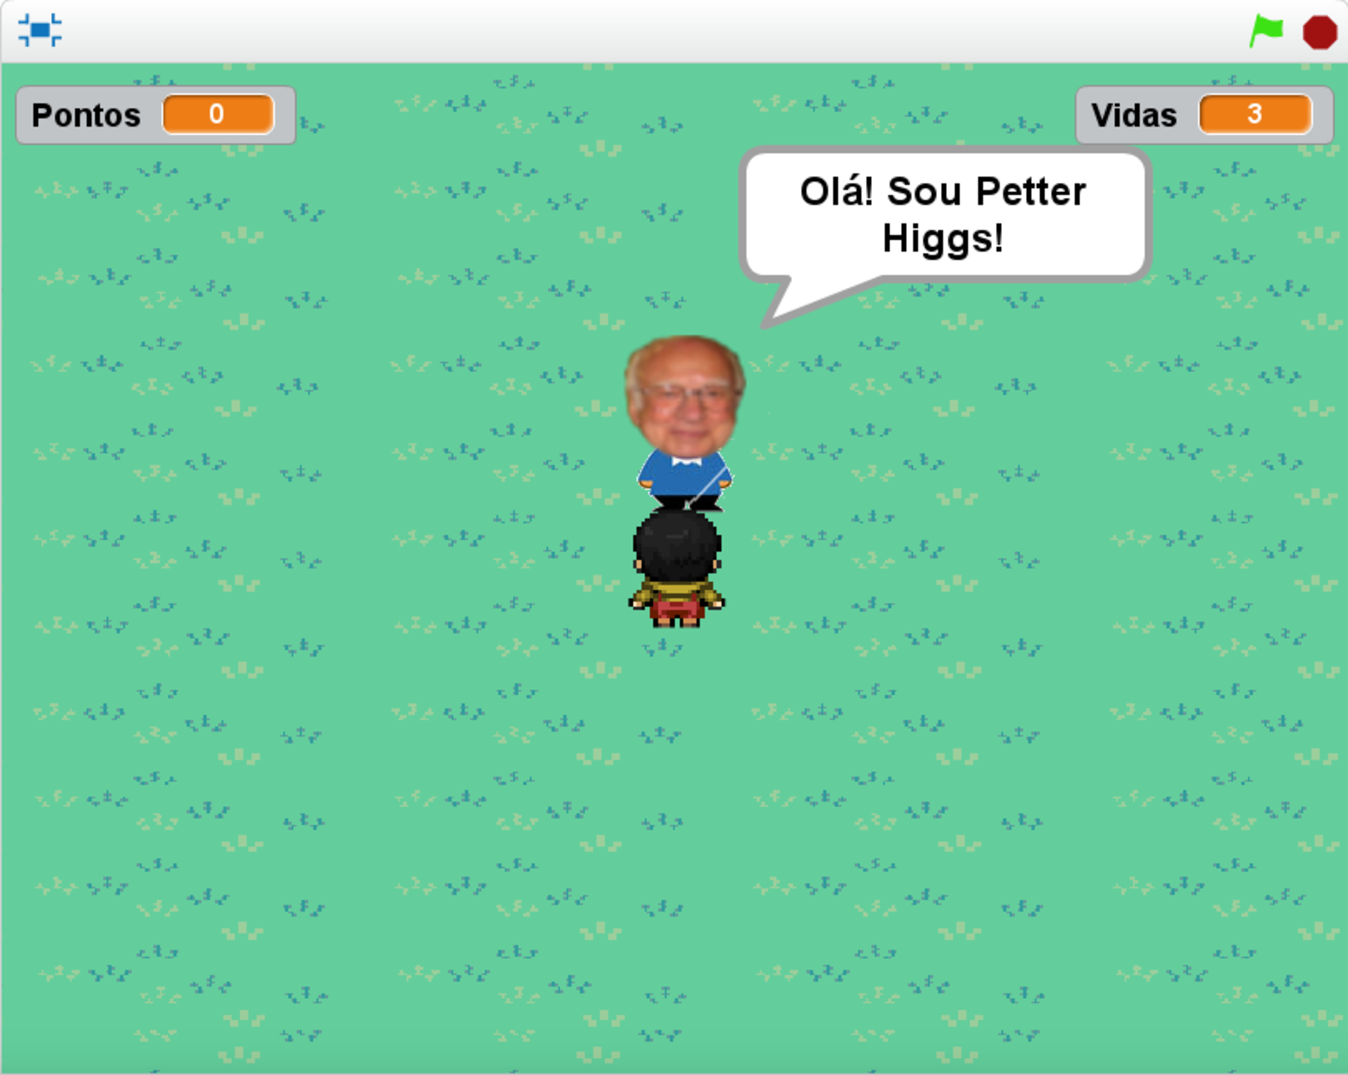
\includegraphics[width=0.65 \textwidth]{Produto/jogo_3}
	\caption{Diálogo com Higgs 1}
	\label{fig:app_a:jogo3}
\end{figure}

\newpage

Quando encontrar o personagem, fique de frente a ele e tecle \aspas{espaço}, Higgs irá perguntar seu nome\footnote{Ao longo do jogo, todos os personagens irão interagir com você a partir do seu nome}, neste momento você deverá escrever seu nome via teclado e apertar a tecla \aspas{enter}.

\begin{figure}[h]
	\centering
	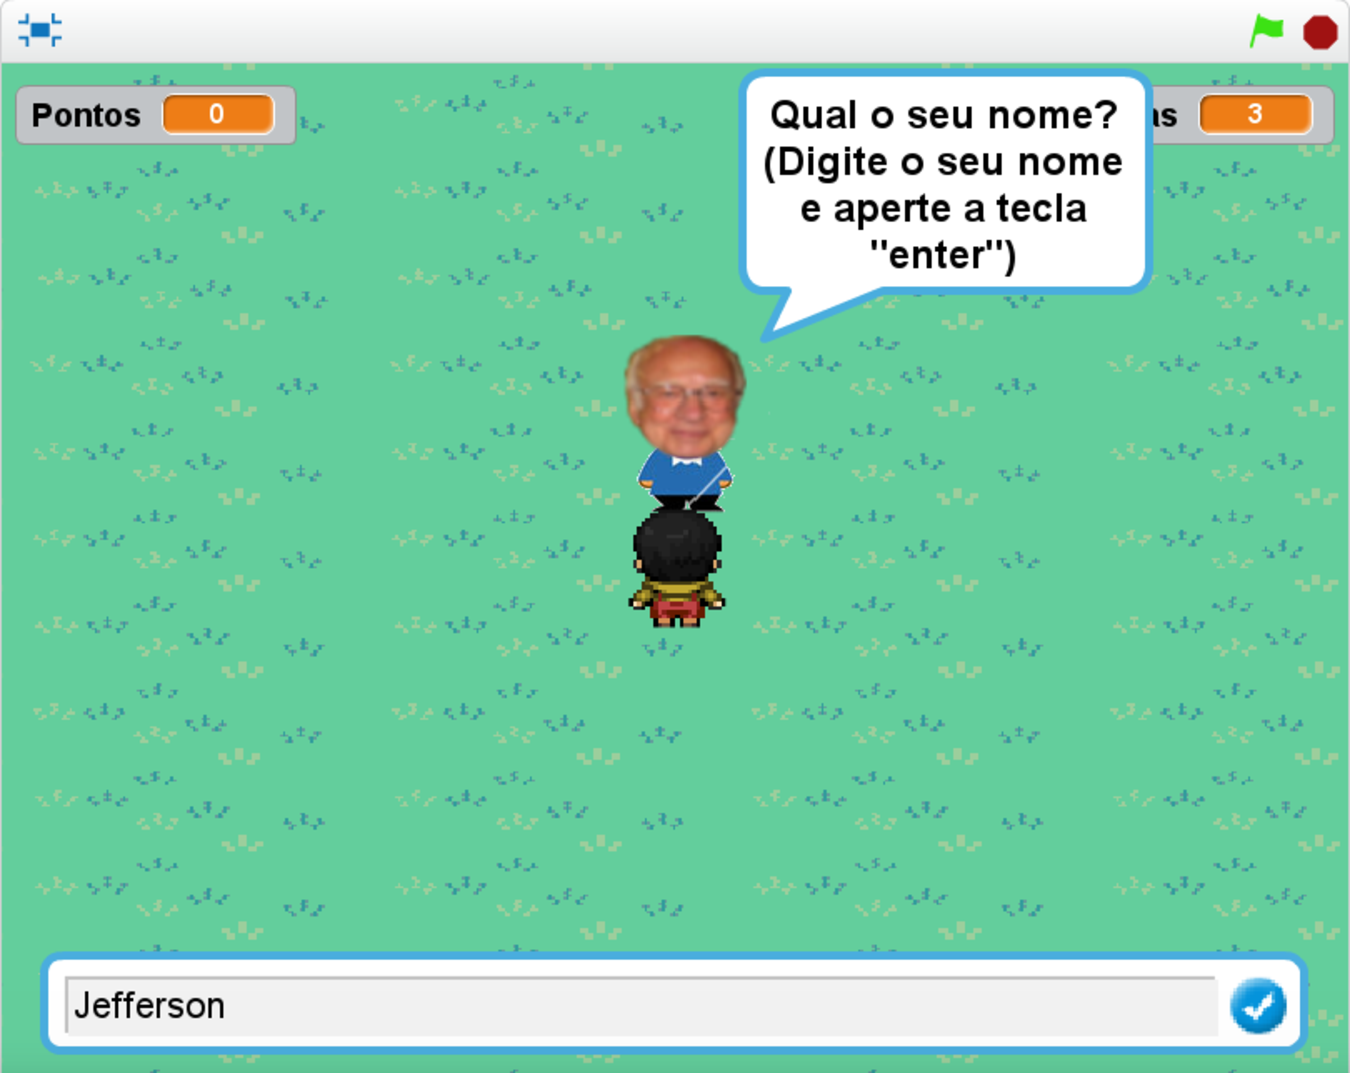
\includegraphics[width=0.65 \textwidth]{Produto/jogo_4}
	\caption{Diálogo com Higgs 2}
	\label{fig:app_a:jogo4}
\end{figure}

Após o diálogo inicial com Higgs, ele mostrará a indicação do próximo passo para concluir a missão.

\begin{figure}[h]
	\centering
	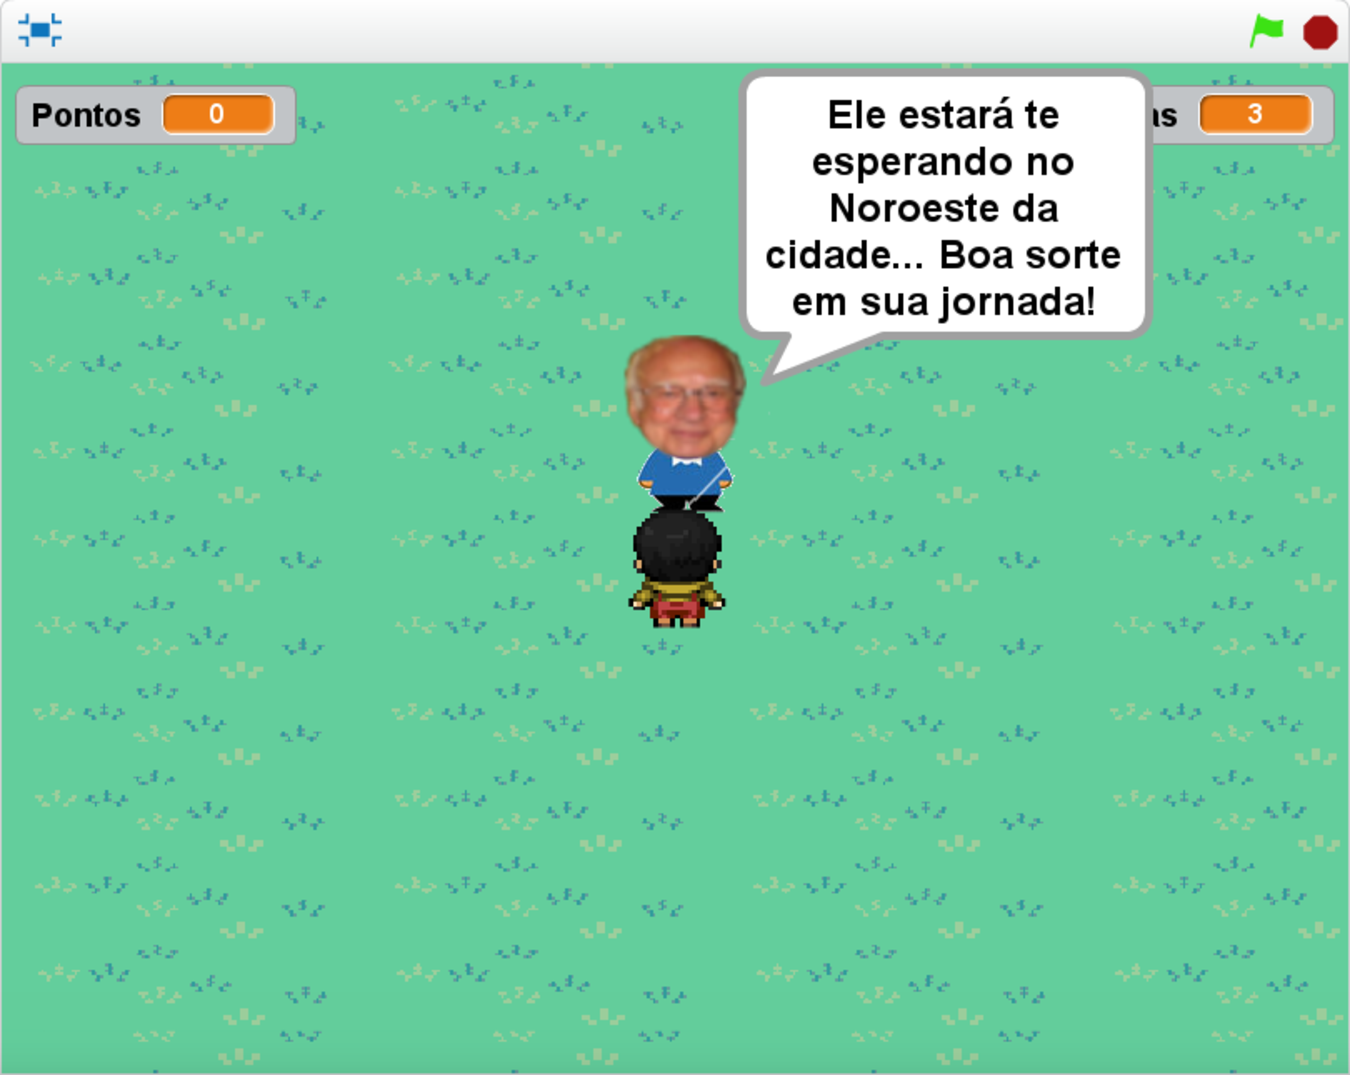
\includegraphics[width=0.65 \textwidth]{Produto/jogo_5}
	\caption{Diálogo com Higgs 3}
	\label{fig:app_a:jogo5}
\end{figure}

\newpage

Ao encontrar com o próximo personagem, Linus Pauling, aperte a tecle novamente \aspas{espaço} para inicial do diálogo.

\begin{figure}[h]
	\centering
	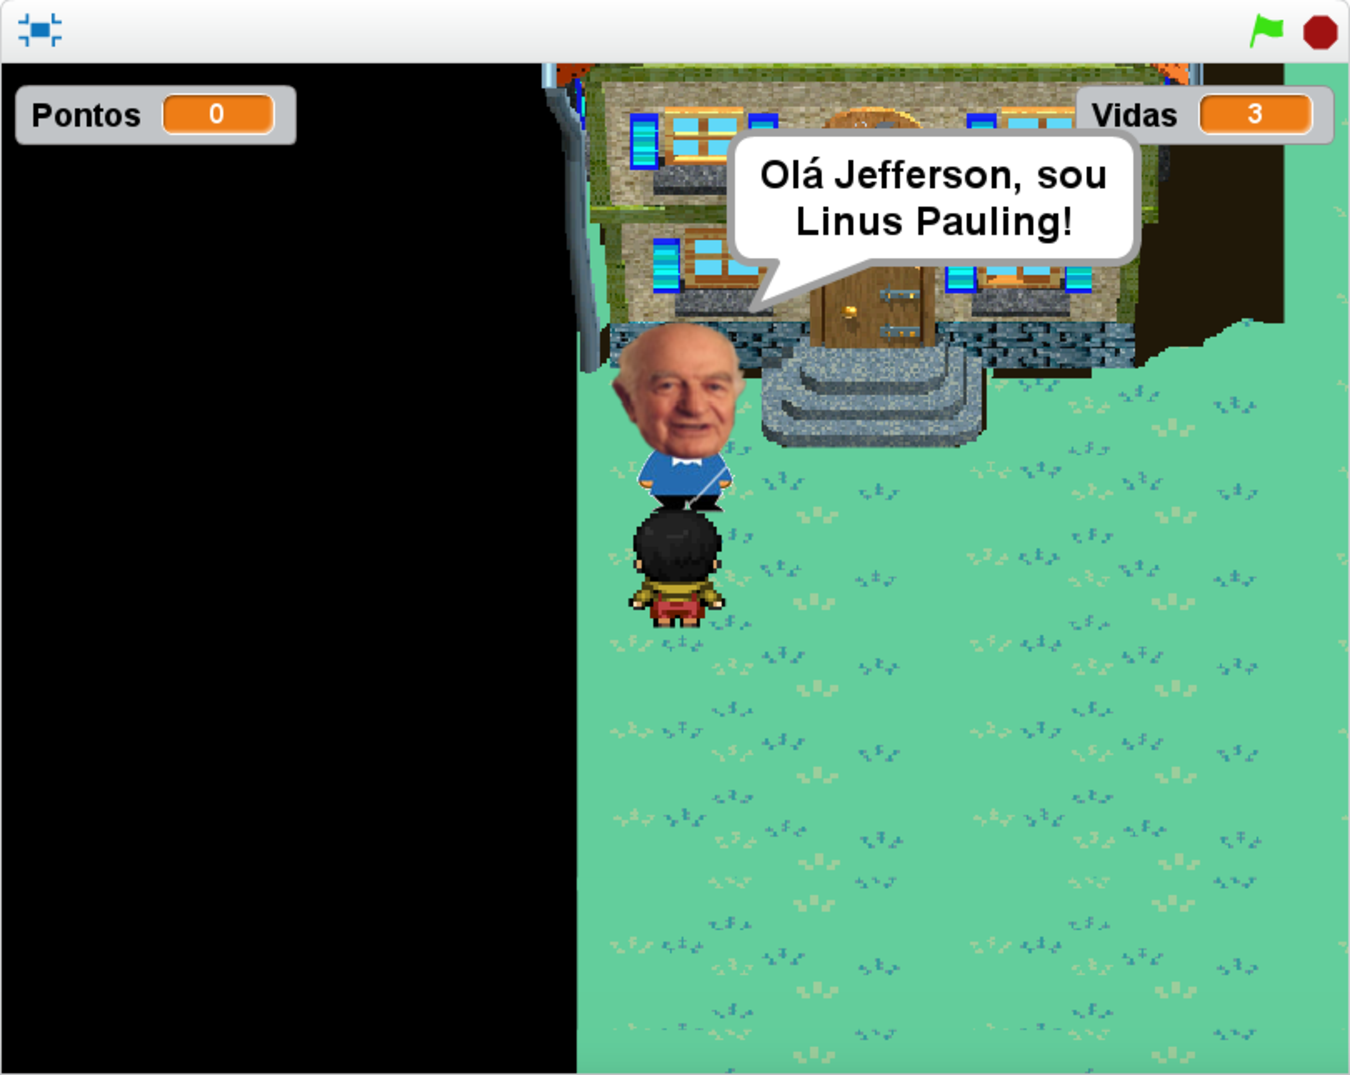
\includegraphics[width=0.65 \textwidth]{Produto/jogo_6}
	\caption{Diálogo com Pauling 1}
	\label{fig:app_a:jogo6}
\end{figure}

Aqui começa as ideias introdutórias da física de partículas elementares.

\begin{figure}[h]
	\centering
	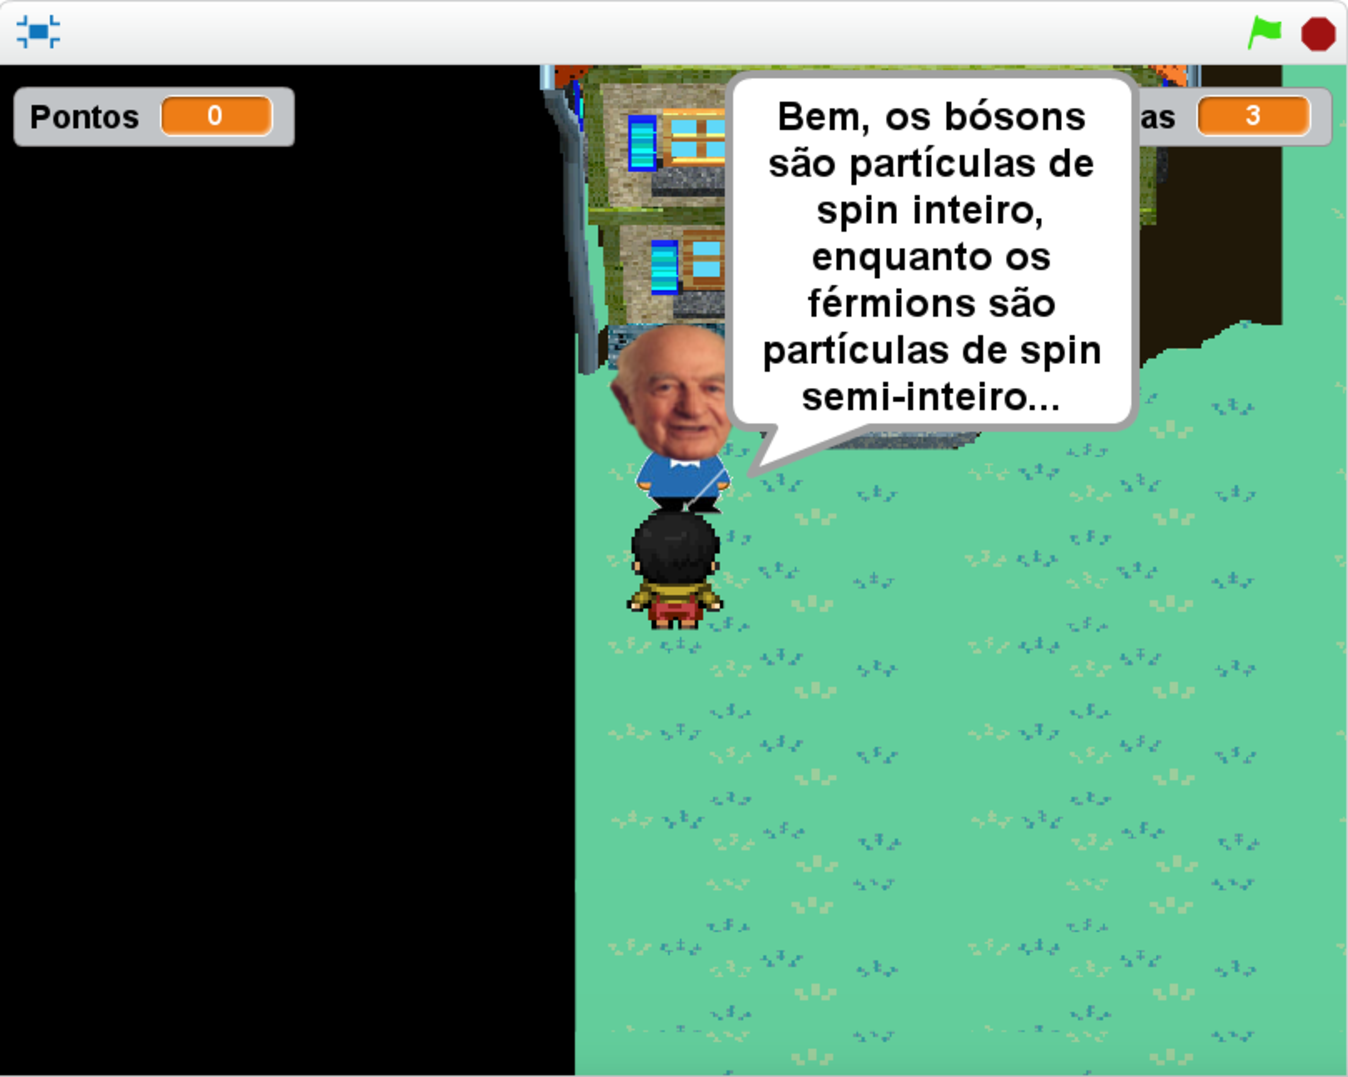
\includegraphics[width=0.65 \textwidth]{Produto/jogo_7}
	\caption{Diálogo com Pauling 2}
	\label{fig:app_a:jogo7}
\end{figure}

\newpage

Após o diálogo, Pauling comentará que você procure o físico César Lattes.

\begin{figure}[h]
	\centering
	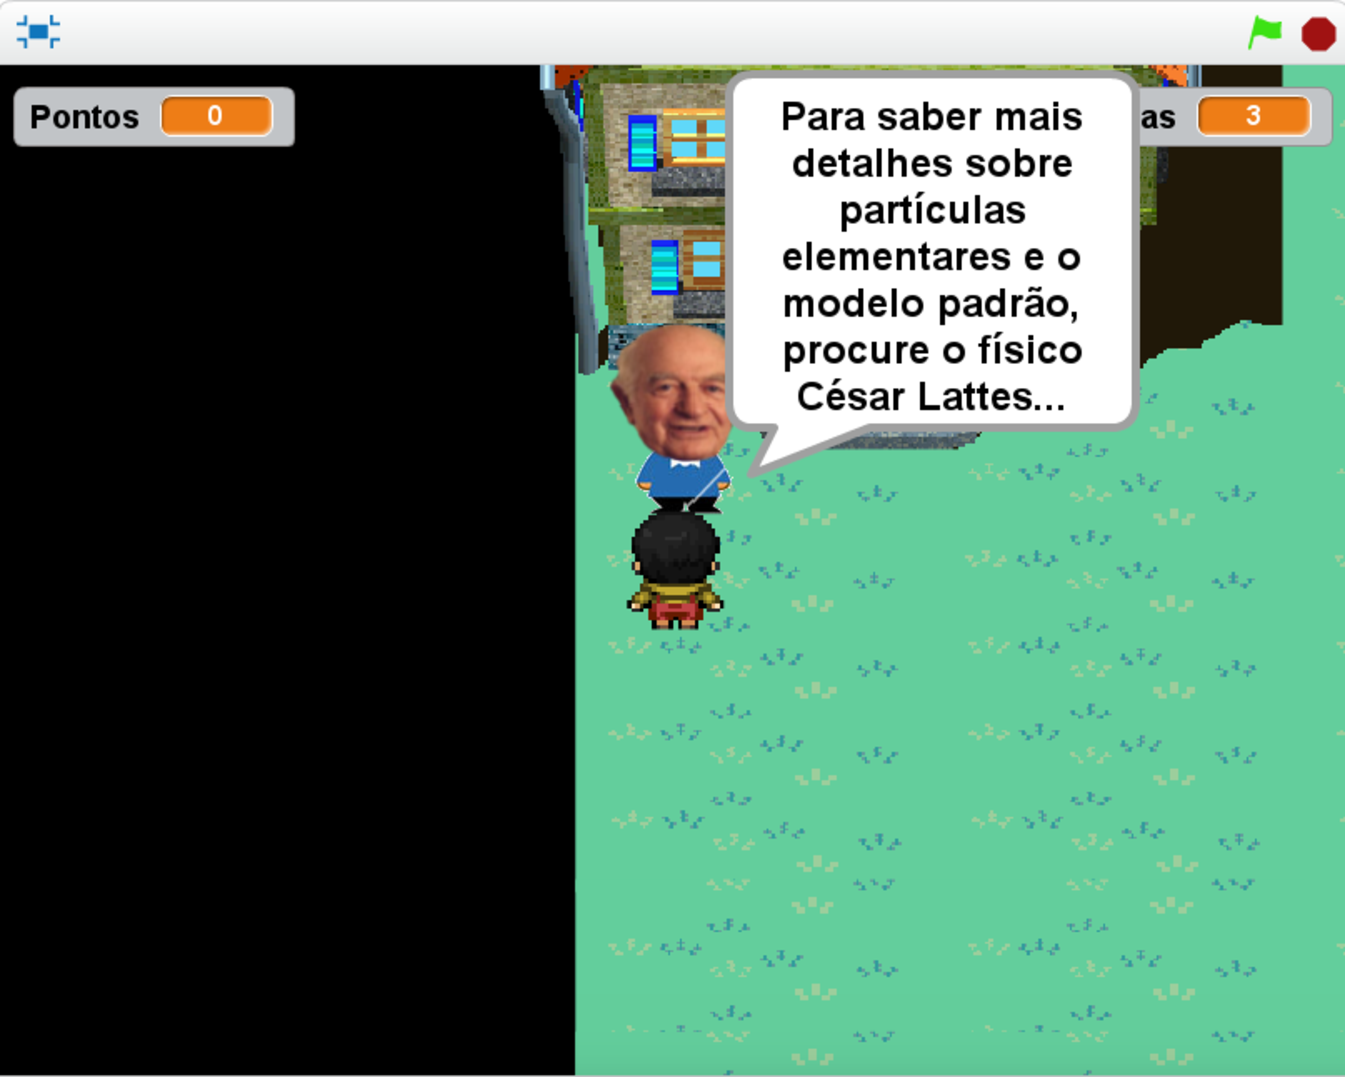
\includegraphics[width=0.65 \textwidth]{Produto/jogo_8}
	\caption{Diálogo com Pauling 3}
	\label{fig:app_a:jogo8}
\end{figure}

Aqui começa o diálogo com Lattes.

\begin{figure}[h]
	\centering
	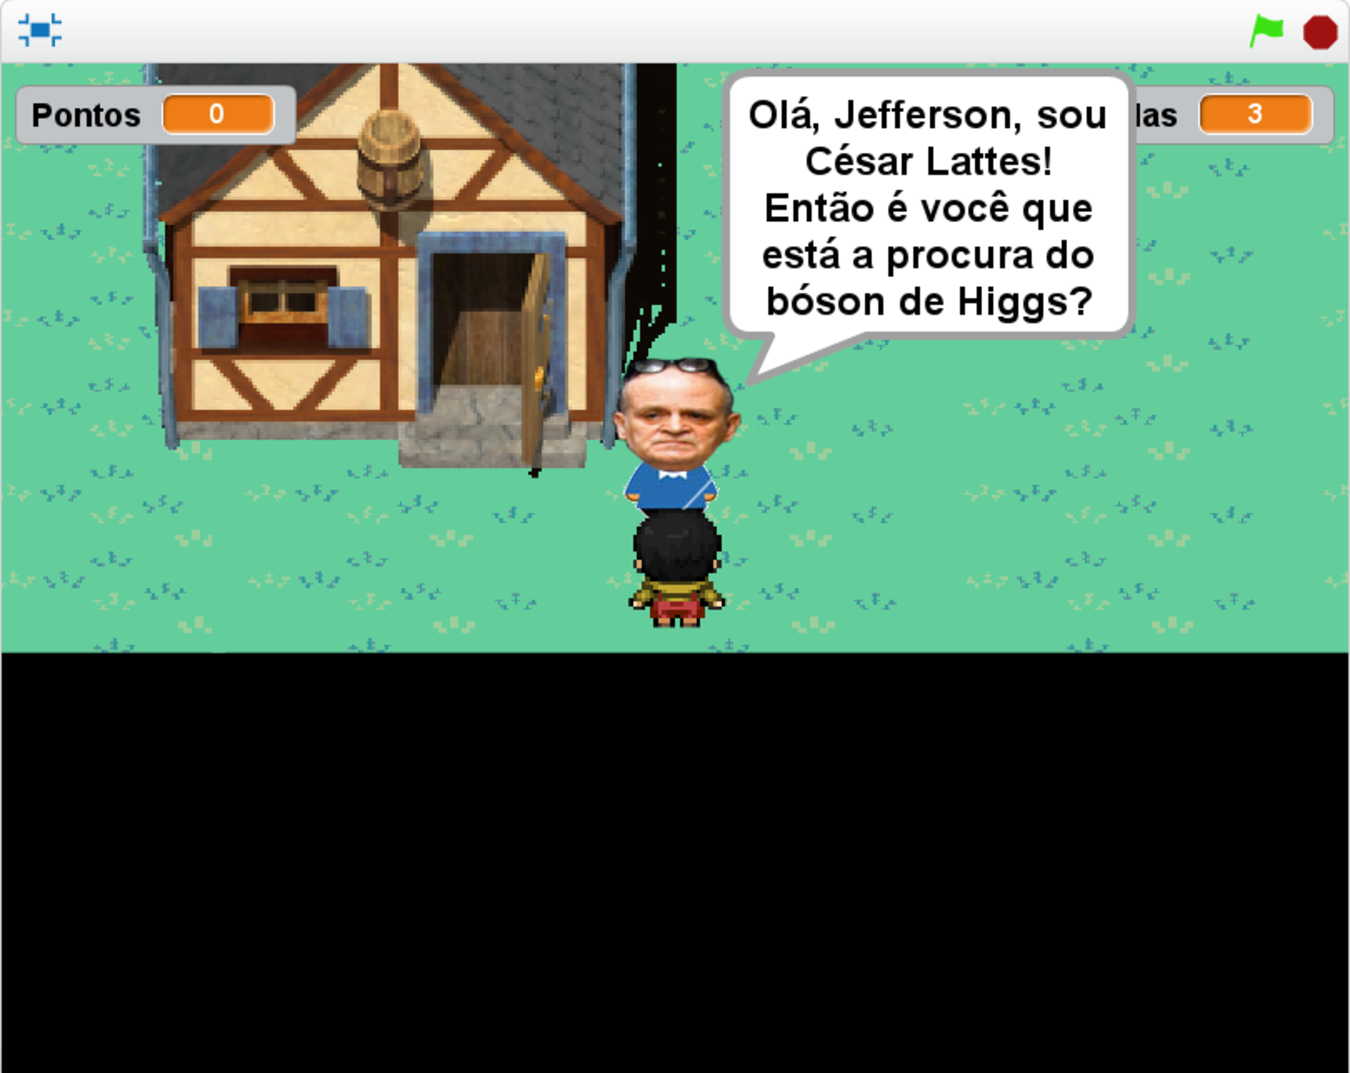
\includegraphics[width=0.65 \textwidth]{Produto/jogo_9}
	\caption{Diálogo com Lattes 1}
	\label{fig:app_a:jogo9}
\end{figure}

\newpage

Após os diálogos, são realizadas o \textit{quiz} referentes ao diálogo dos personagens.

\begin{figure}[h]
	\centering
	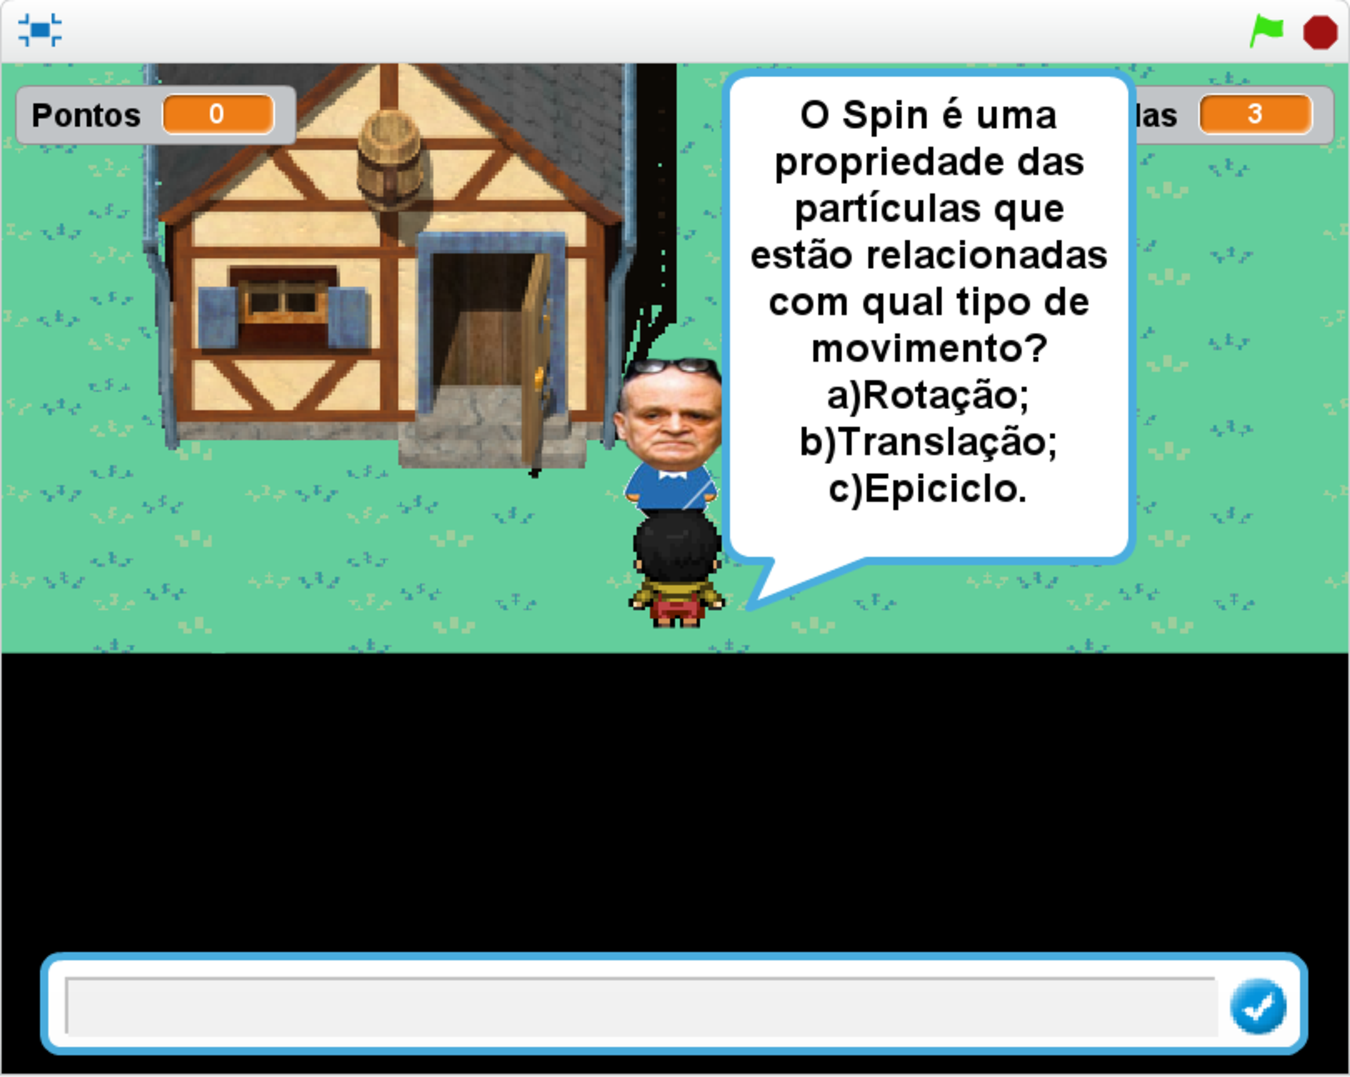
\includegraphics[width=0.65 \textwidth]{Produto/jogo_10}
	\caption{Diálogo com Lattes 2}
	\label{fig:app_a:jogo10}
\end{figure}

Conforme acerte as perguntas, seus pontos aumentam.

\begin{figure}[h]
	\centering
	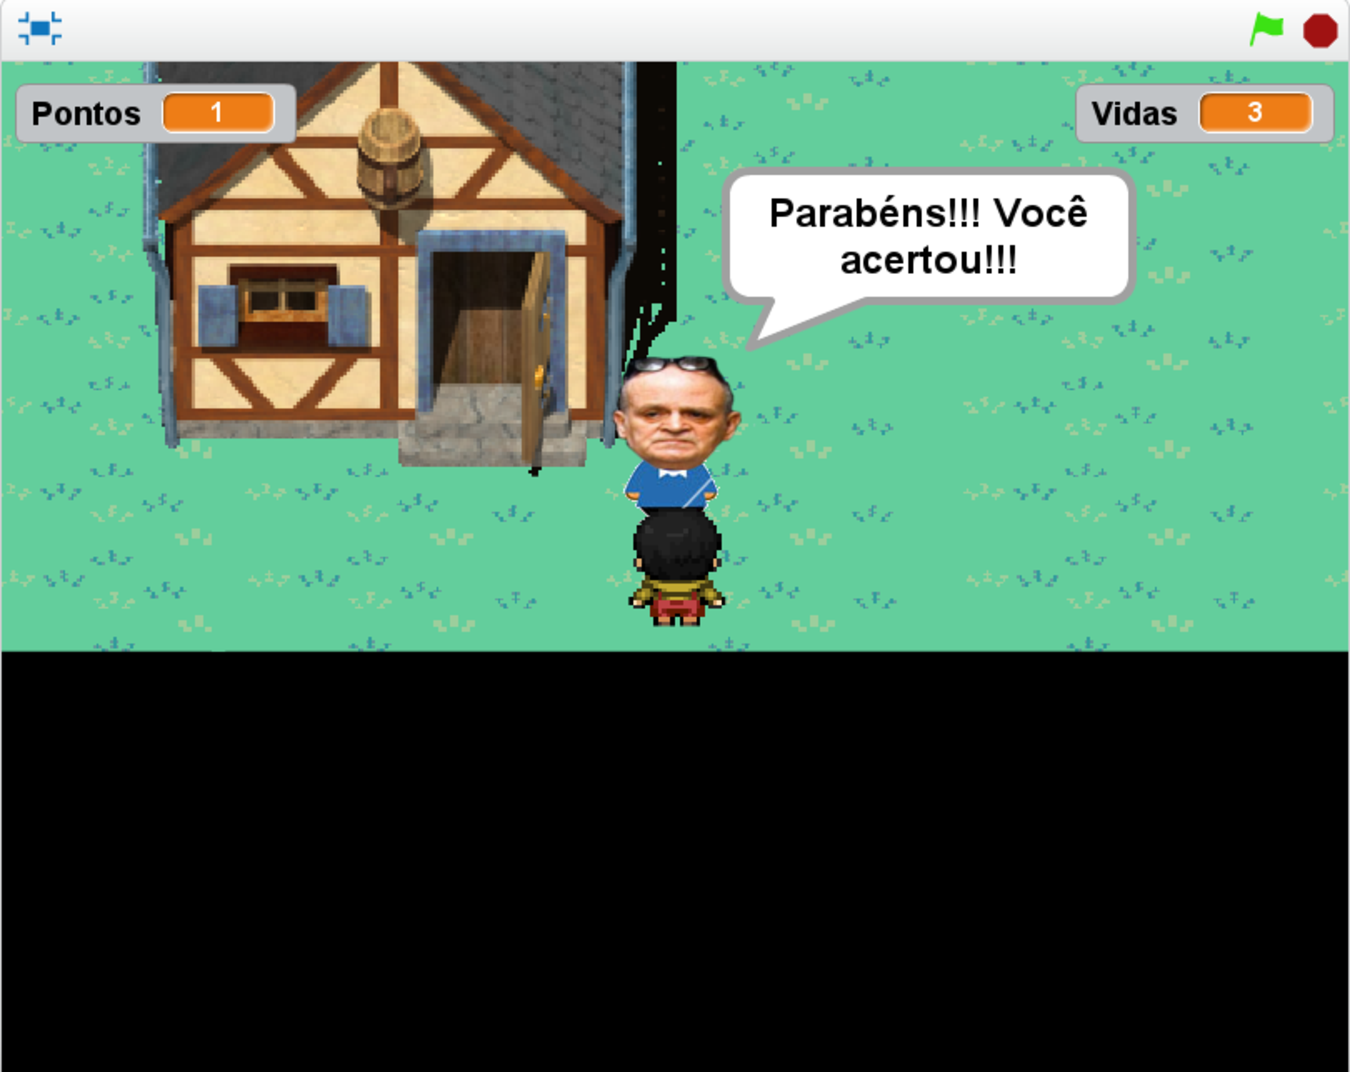
\includegraphics[width=0.65 \textwidth]{Produto/jogo_11}
	\caption{Diálogo com Lattes 3}
	\label{fig:app_a:jogo11}
\end{figure}

\newpage

Caso erre, você deixa de ganhar a pontuação referente à pergunta.

\begin{figure}[h]
	\centering
	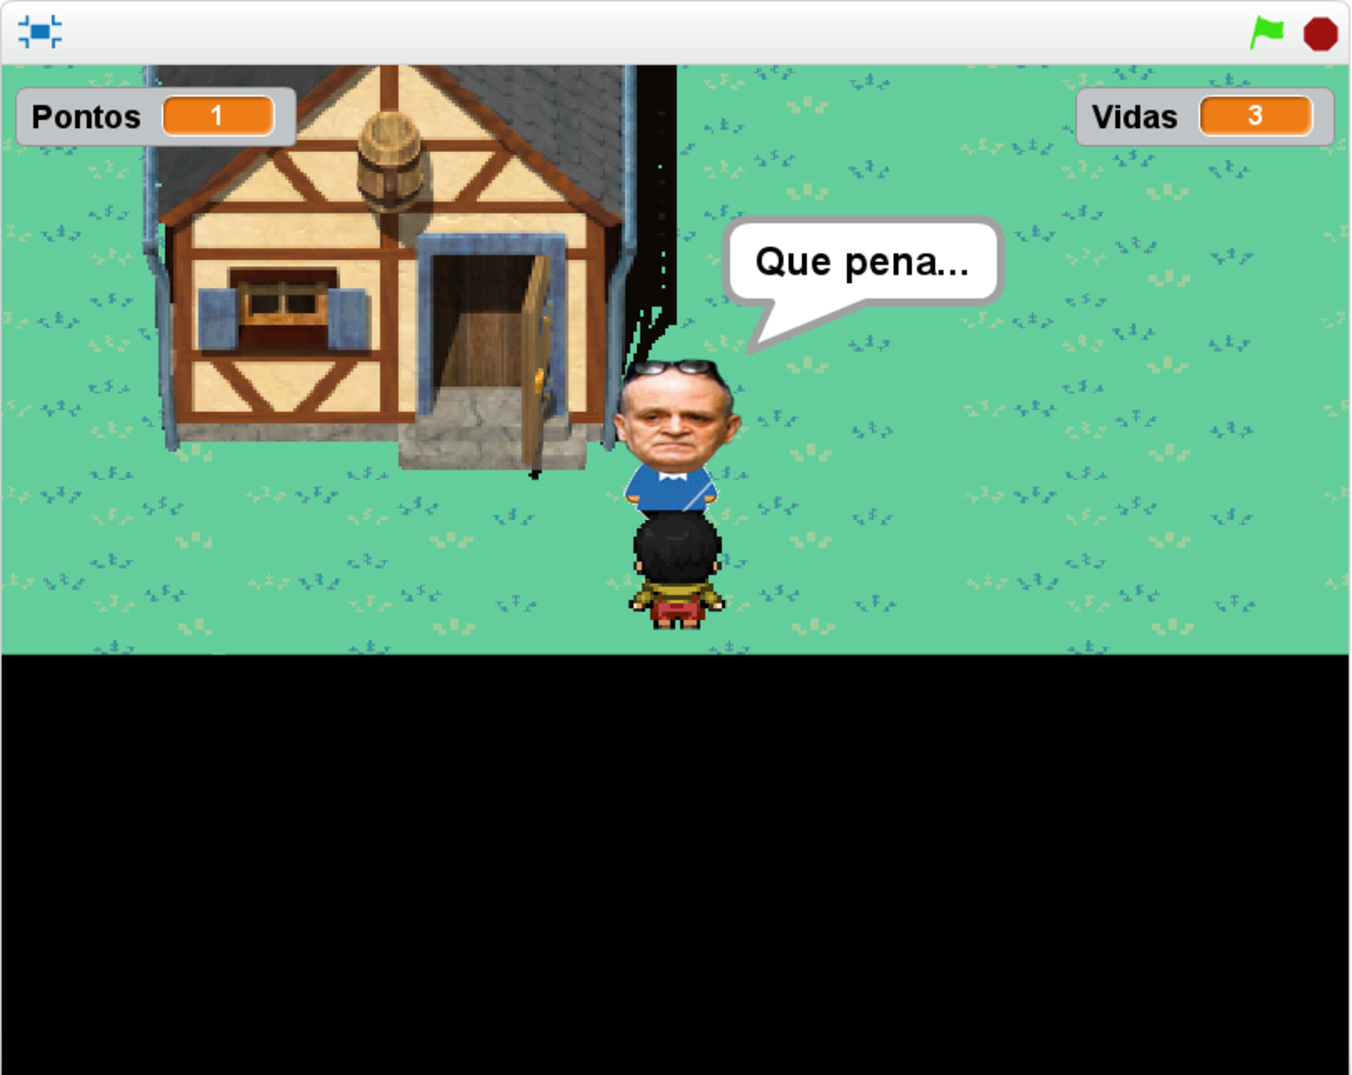
\includegraphics[width=0.65 \textwidth]{Produto/jogo_12}
	\caption{Diálogo com Lattes 3}
	\label{fig:app_a:jogo12}
\end{figure}

Aqui um exemplo de pergunta sobre o modelo padrão.

\begin{figure}[h]
	\centering
	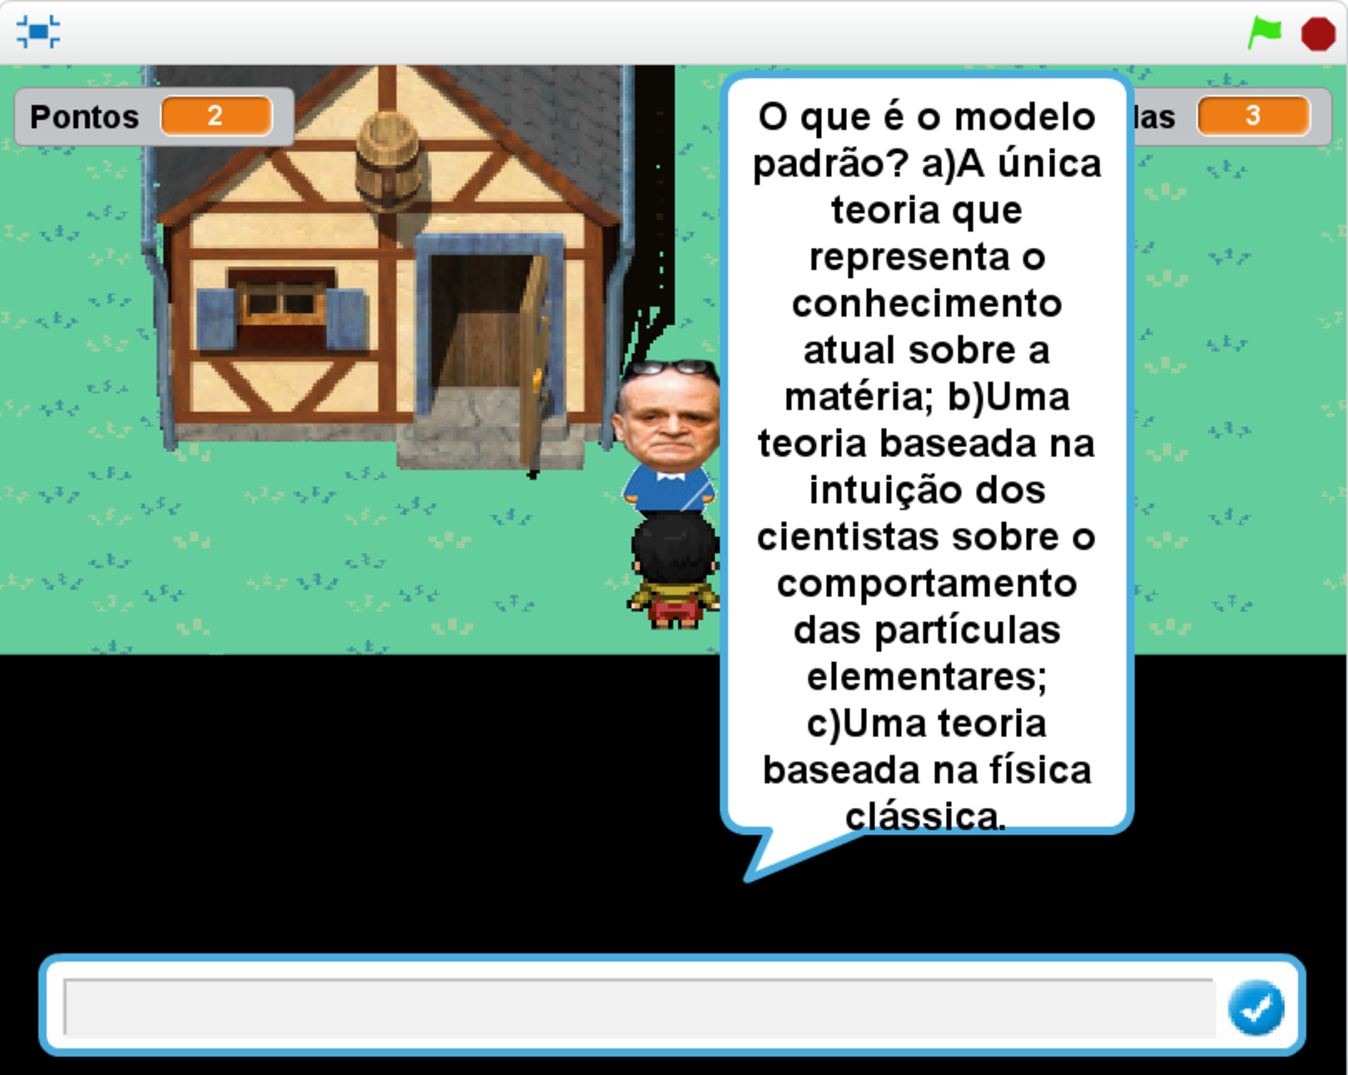
\includegraphics[width=0.65 \textwidth]{Produto/jogo_13}
	\caption{Diálogo com Lattes 4}
	\label{fig:app_a:jogo13}
\end{figure}

\newpage

Lattes comentará que você procure Einstein.

\begin{figure}[h]
	\centering
	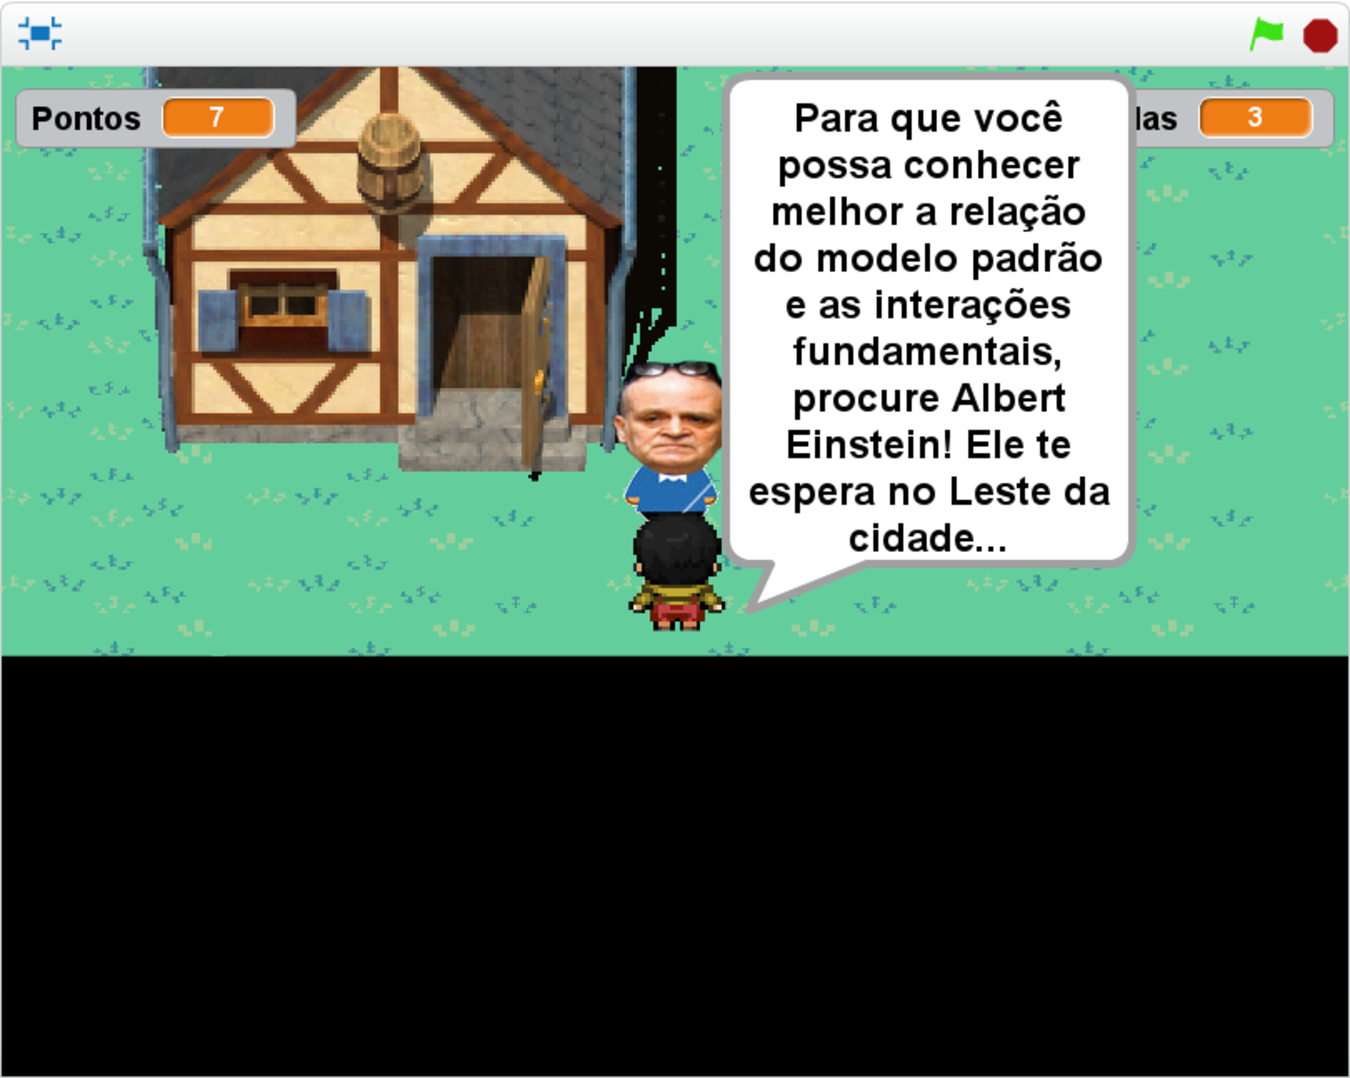
\includegraphics[width=0.65 \textwidth]{Produto/jogo_14}
	\caption{Diálogo com Lattes 5}
	\label{fig:app_a:jogo14}
\end{figure}

Após o encontro com Einstein, inicia-se o diálogo.

\begin{figure}[h]
	\centering
	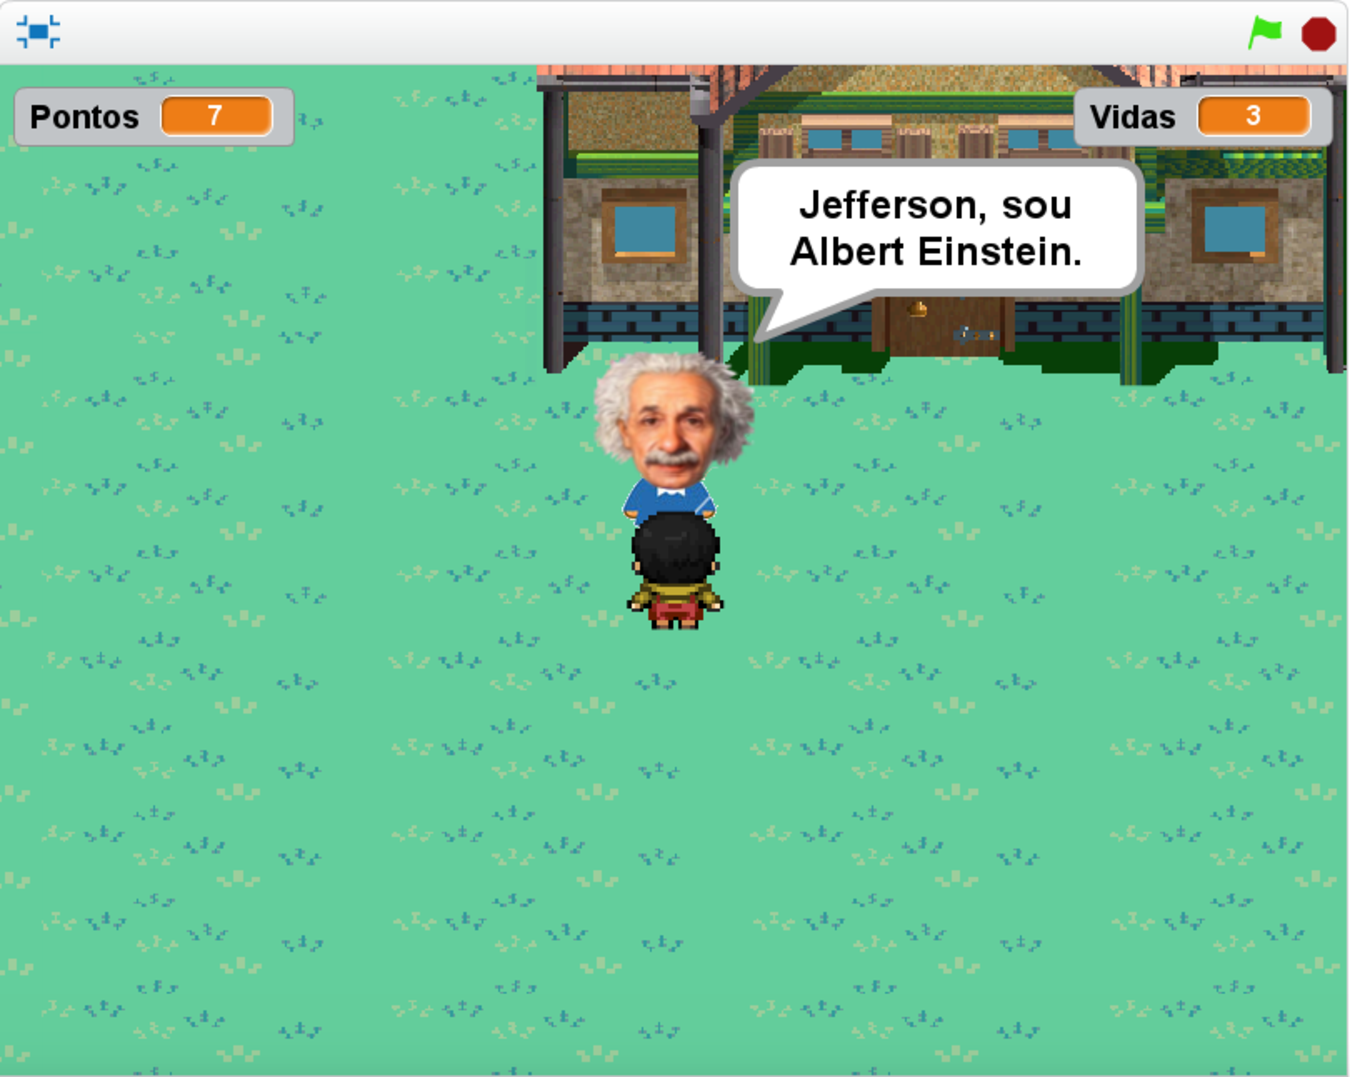
\includegraphics[width=0.65 \textwidth]{Produto/jogo_15}
	\caption{Diálogo com Einstein 1}
	\label{fig:app_a:jogo15}
\end{figure}

\newpage

Após alguns diálogos, Einstein realiza algumas perguntas sobre interações fundamentais.

\begin{figure}[h]
	\centering
	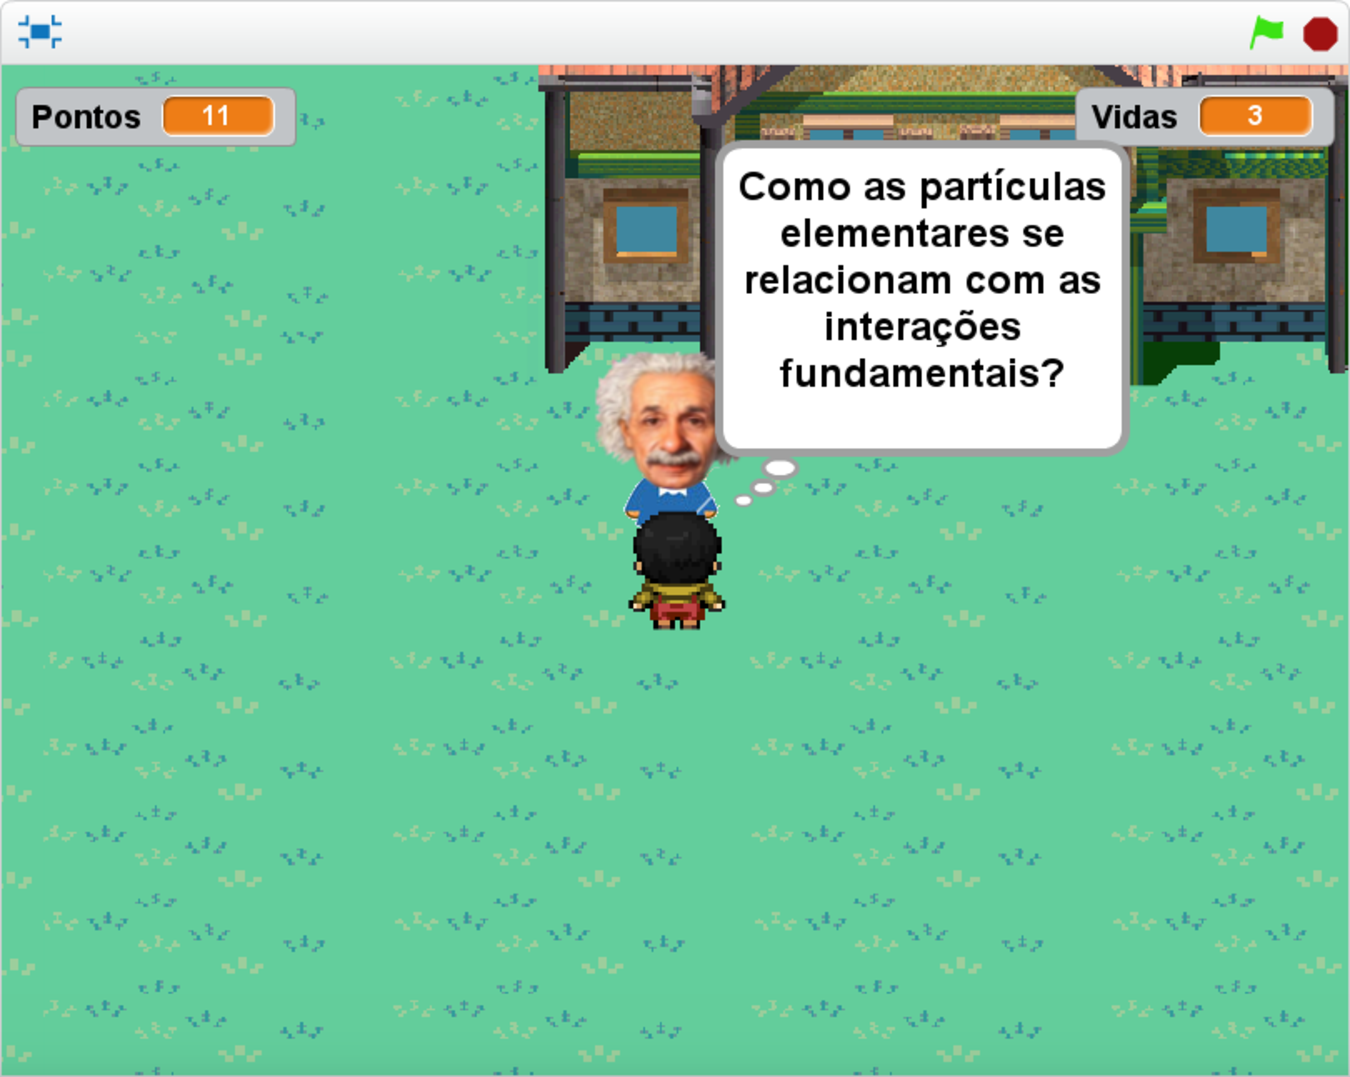
\includegraphics[width=0.65 \textwidth]{Produto/jogo_16}
	\caption{Diálogo com Einstein 2}
	\label{fig:app_a:jogo16}
\end{figure}


Após o diálogo com Einstein, você deverá encontrar novamente com Peter Higgs, que fará mais algumas perguntas...

\begin{figure}[h]
	\centering
	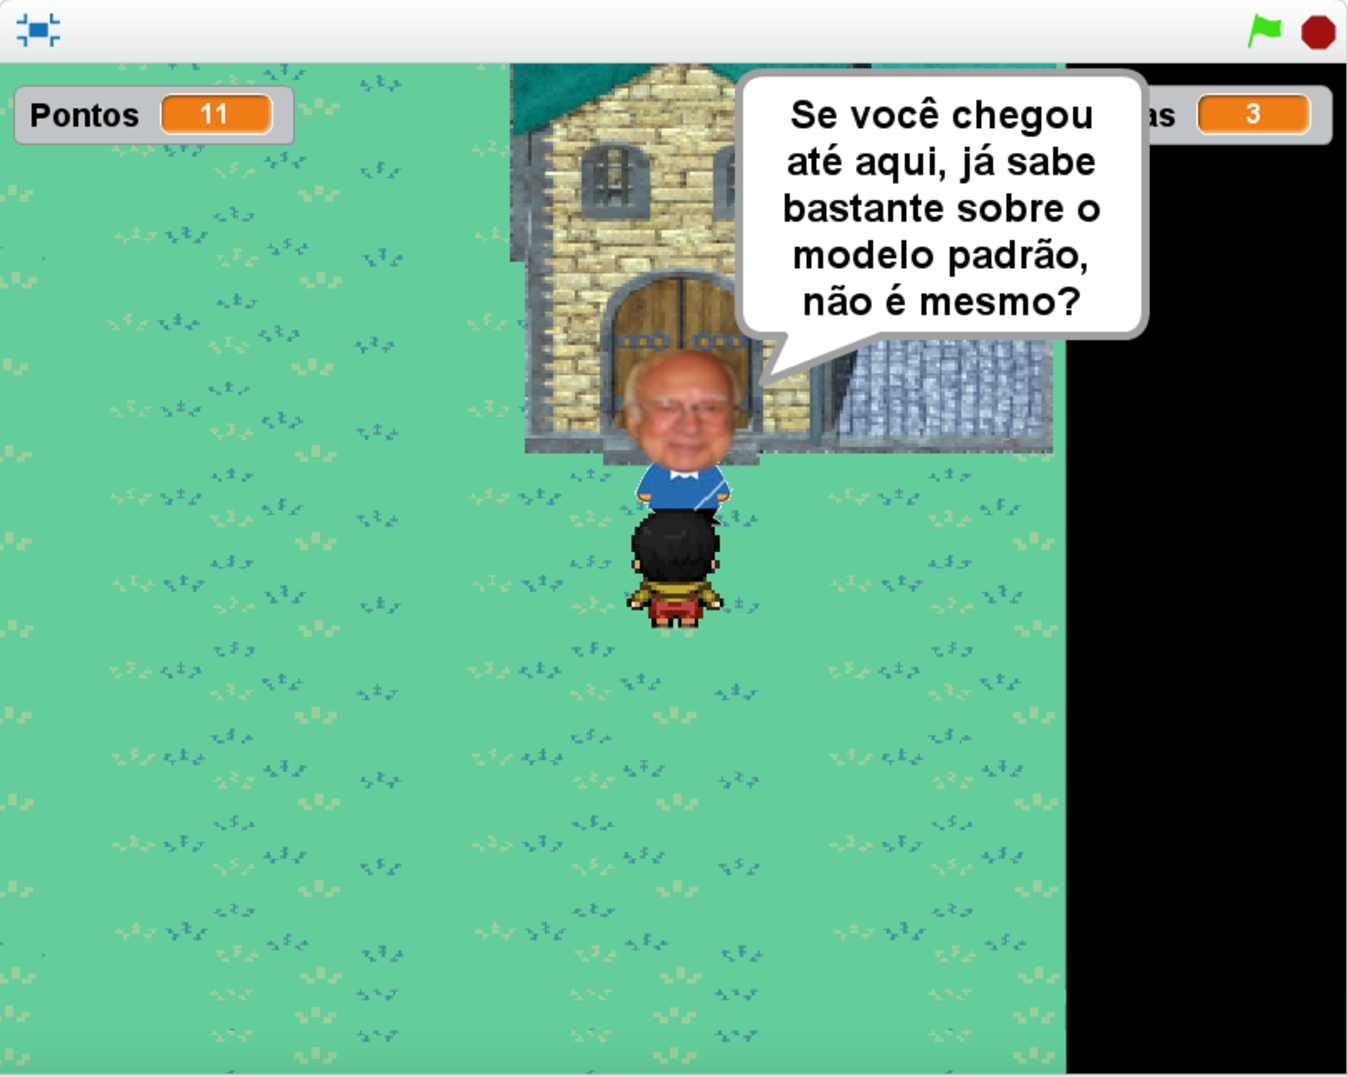
\includegraphics[width=0.65 \textwidth]{Produto/jogo_17}
	\caption{Diálogo final com Higgs 1}
	\label{fig:app_a:jogo17}
\end{figure}

\newpage

Aqui, Higgs explica sobre a última missão...

\begin{figure}[h]
	\centering
	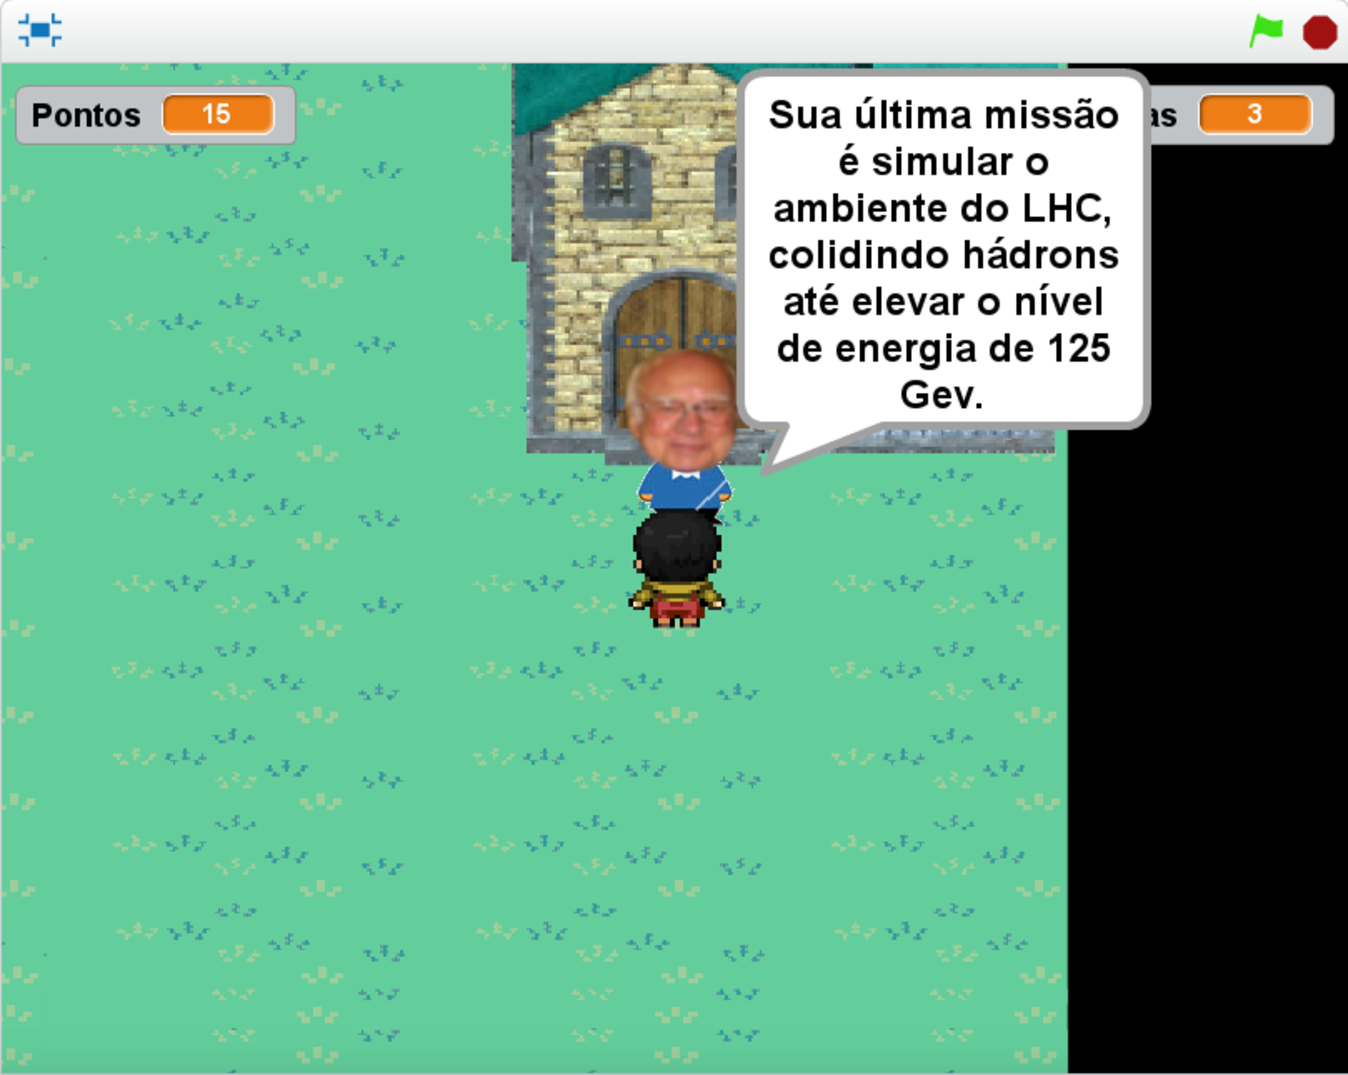
\includegraphics[width=0.65 \textwidth]{Produto/jogo_18}
	\caption{Diálogo final com Higgs 2}
	\label{fig:app_a:jogo18}
\end{figure}

Por fim, chegamos na reta final...

\begin{figure}[h]
	\centering
	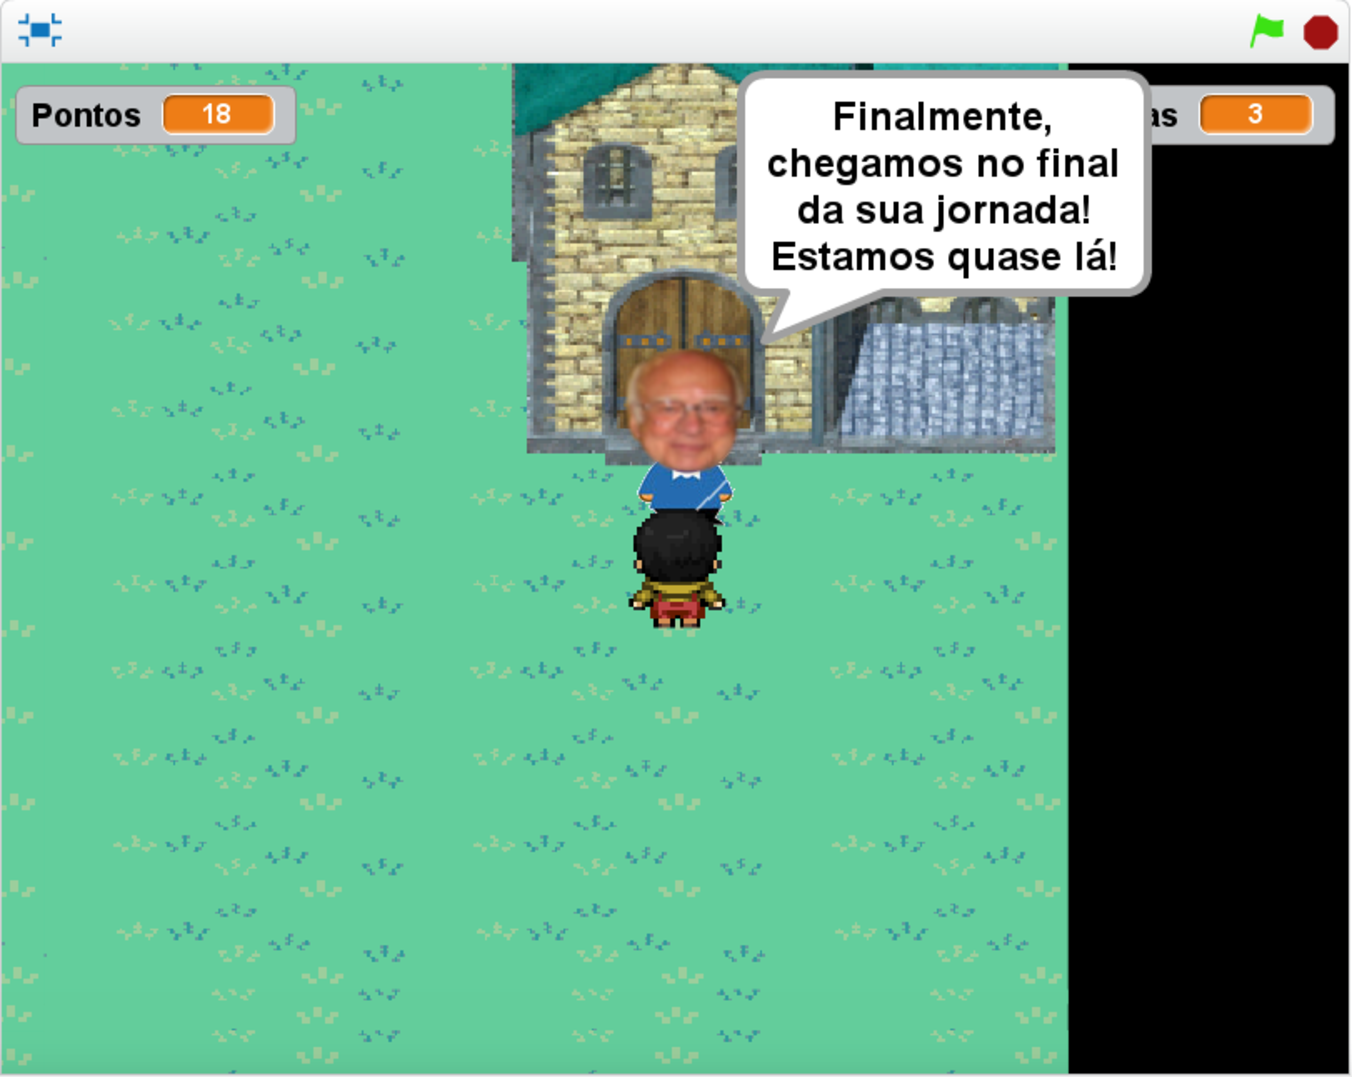
\includegraphics[width=0.65 \textwidth]{Produto/jogo_19}
	\caption{Diálogo final com Higgs 3}
	\label{fig:app_a:jogo19}
\end{figure}

\newpage

\section{A Missão Final}

Inicia-se a simulação da colisão de hádrons.

\begin{figure}[h]
	\centering
	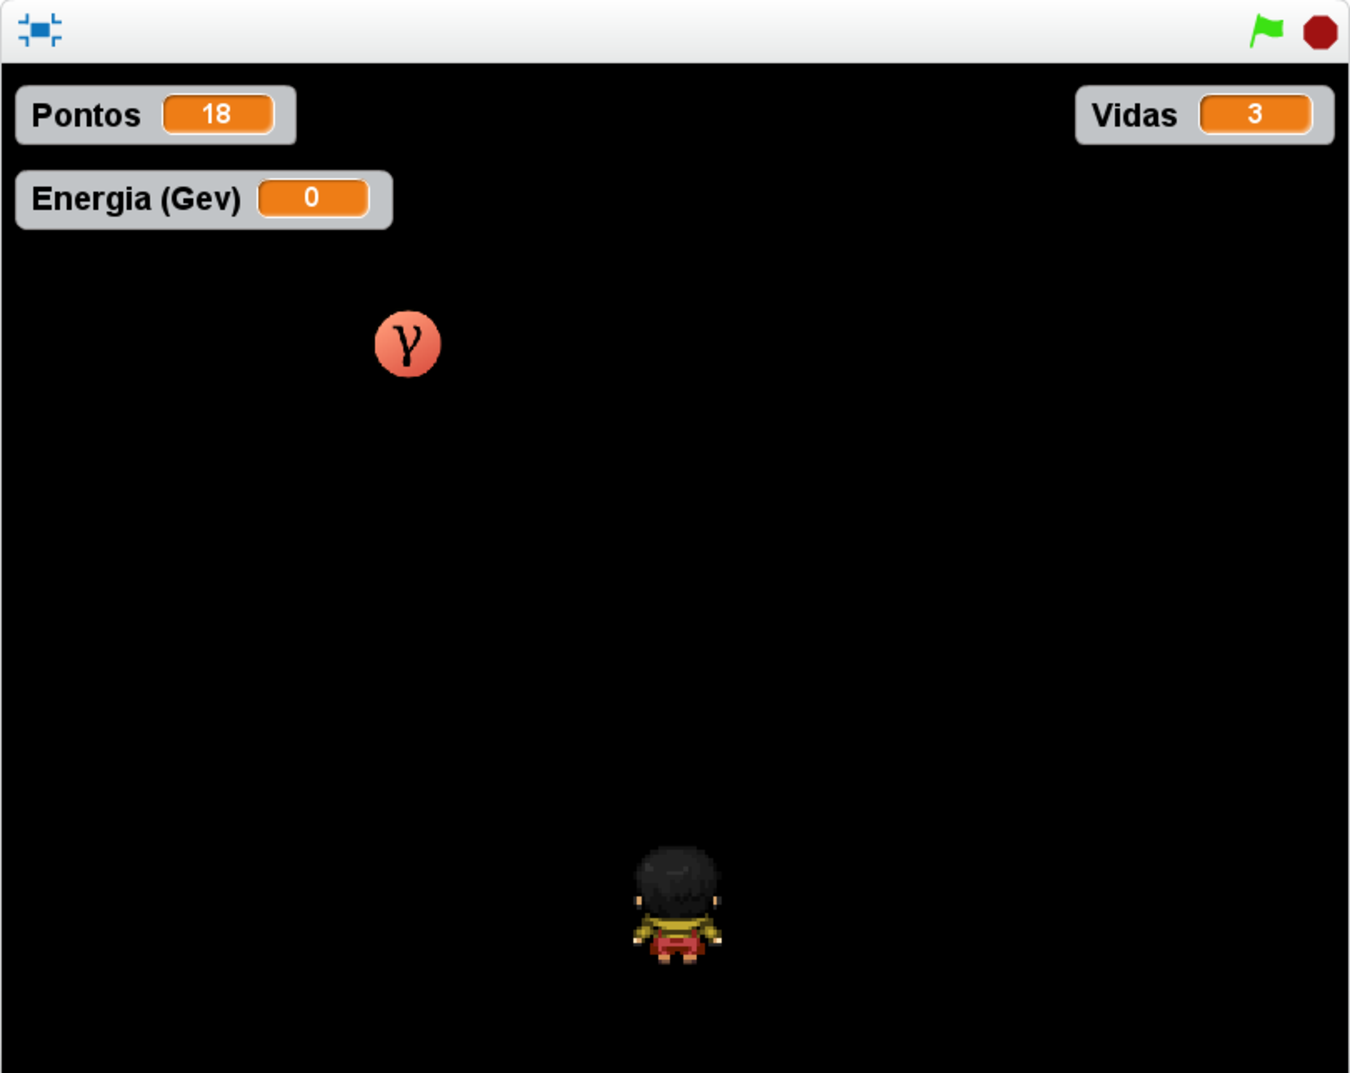
\includegraphics[width=0.65 \textwidth]{Produto/final1}
	\caption{Fase final - parte 1}
	\label{fig:app_a:final1}
\end{figure}

Nesta etapa, você perceberá que irá descer várias partículas, dentre elas: o fóton, o elétron e o próton.

\begin{figure}[h]
	\centering
	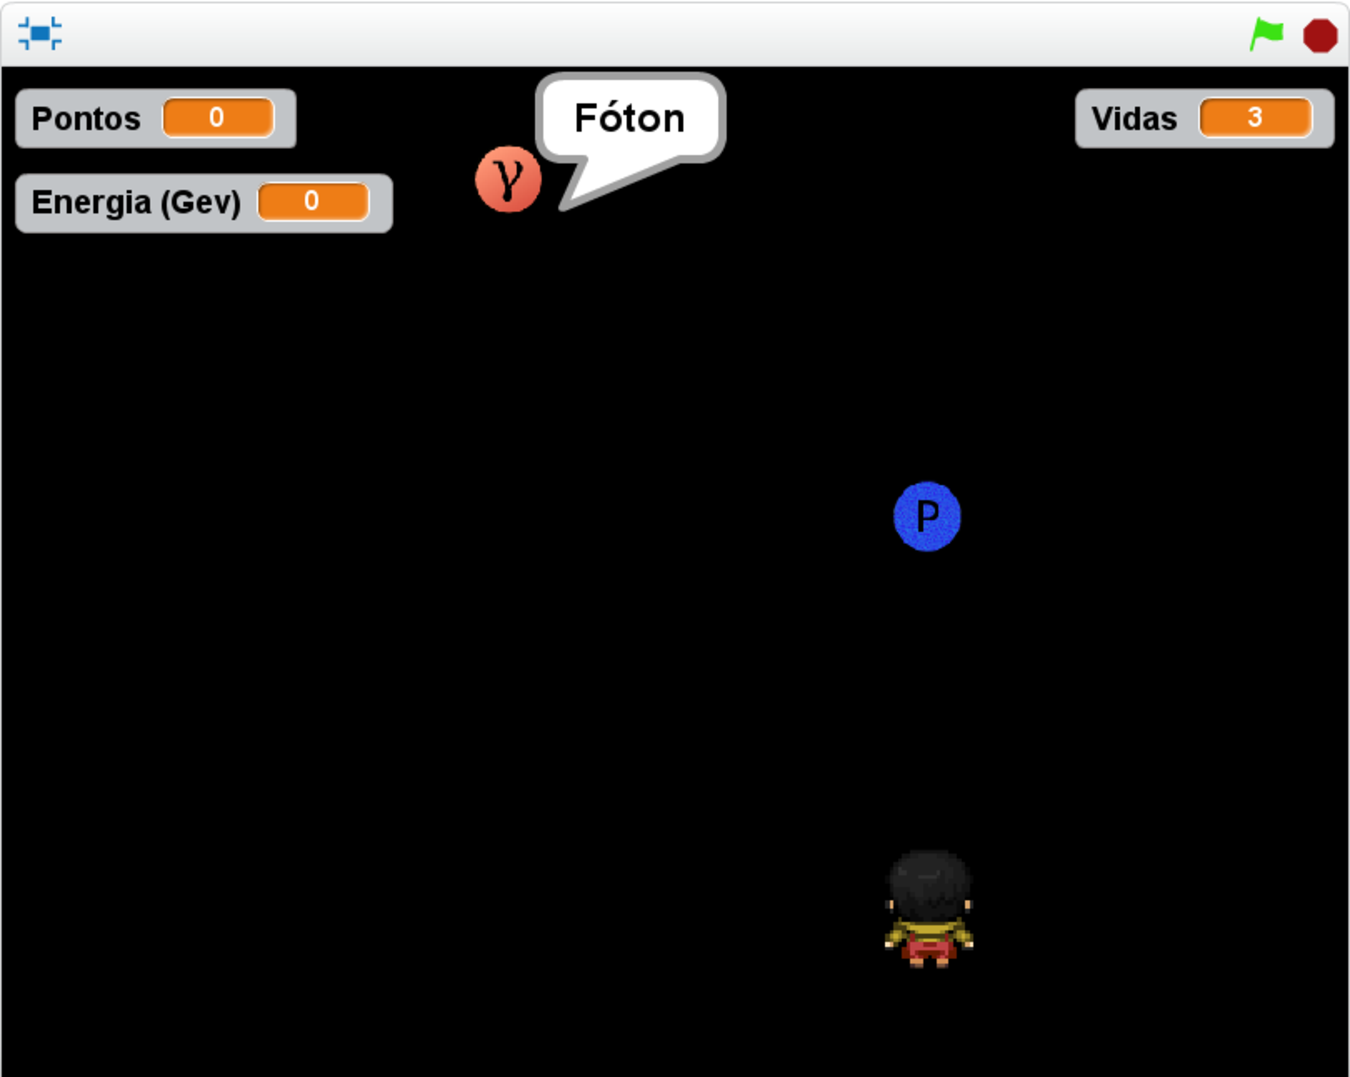
\includegraphics[width=0.65 \textwidth]{Produto/final2}
	\caption{Fase final - parte 2}
	\label{fig:app_a:final2}
\end{figure}

\newpage

O objetivo desta última missão é a colisão do próton (que está com o personagem principal) com os prótons que descem sobre a tela.

Para cada acerto, o parâmetro de energia aumenta 25 GeV, enquanto que se você colidir com as partículas de forma inadequada ou se alguma partícula colidir em você, perderás uma vida.

\begin{figure}[h]
	\centering
	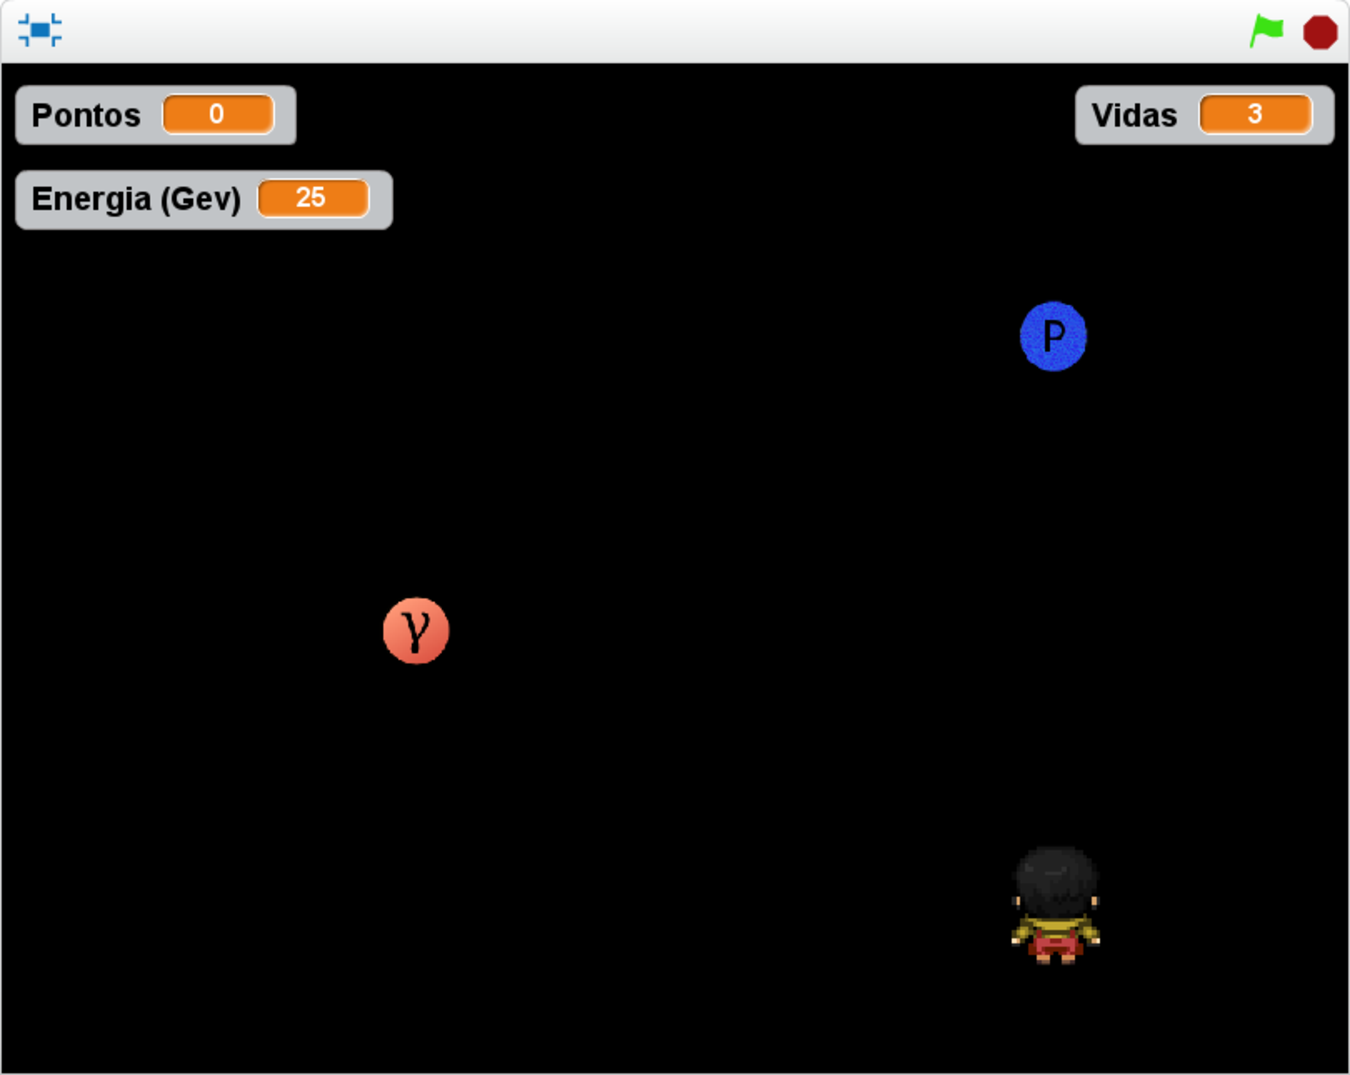
\includegraphics[width=0.65 \textwidth]{Produto/final3}
	\caption{Fase final - parte 3}
	\label{fig:app_a:final3}
\end{figure}


Caso consiga chegar em nível de energia de 125 GeV, você alcançará o objetivo e detectará o bóson de Higgs.

\begin{figure}[h]
	\centering
	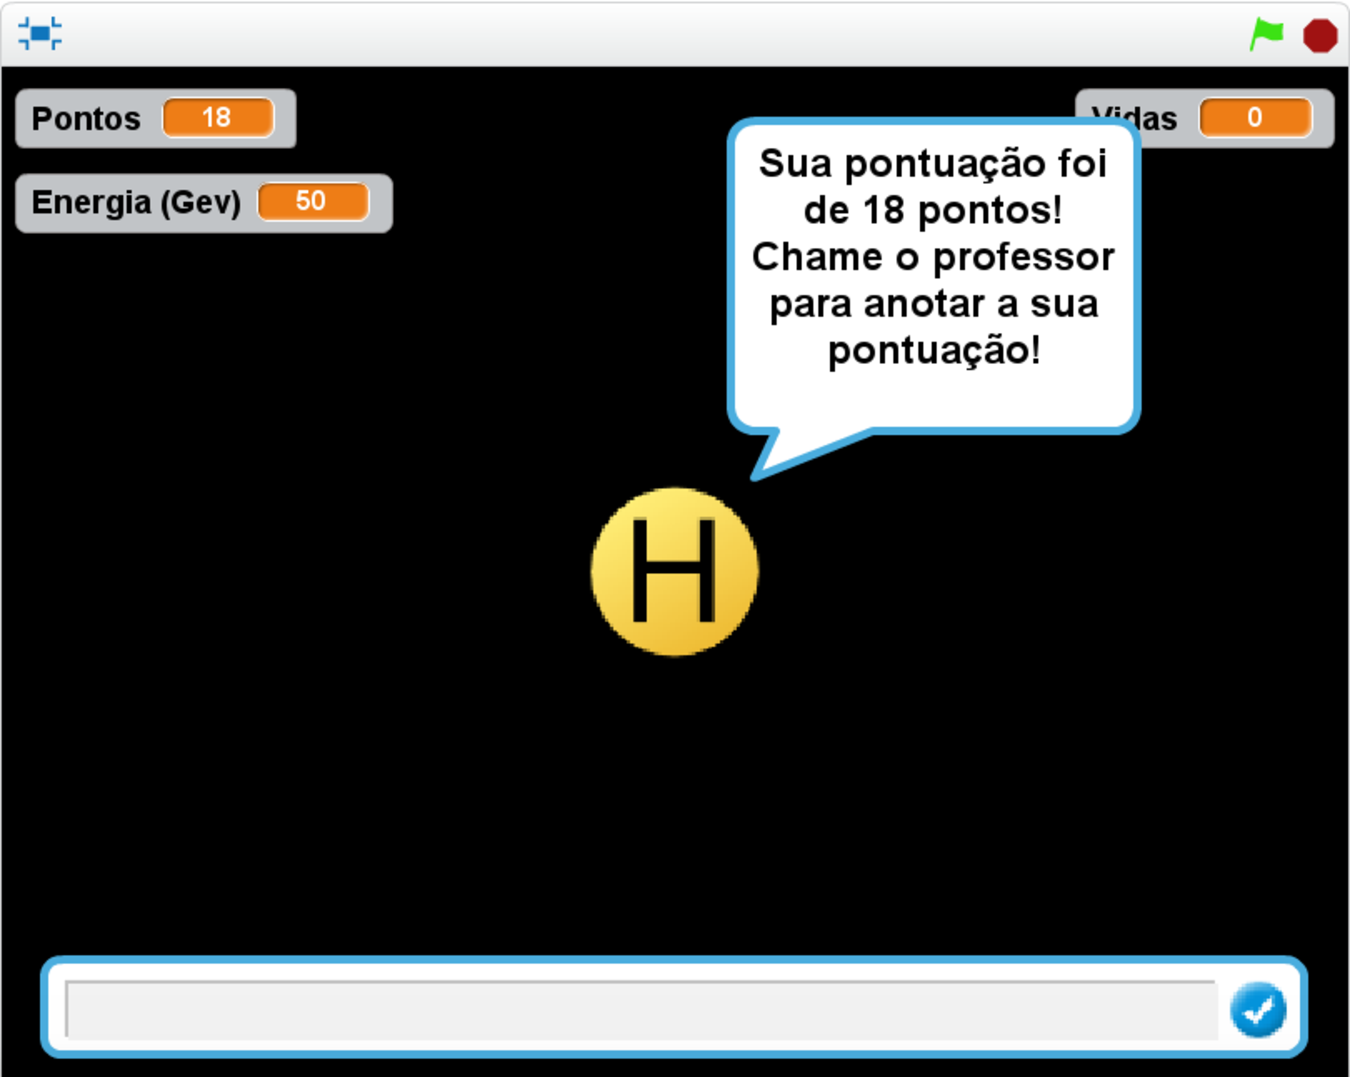
\includegraphics[width=0.65 \textwidth]{Produto/final4}
	\caption{Fase final - parte 4}
	\label{fig:app_a:final4}
\end{figure}




%----------------------------------------------------------------------------------------
%	BIBLIOGRAPHY
%----------------------------------------------------------------------------------------
\chapterimage{sumario.pdf} % Chapter heading image
\chapter*{Referências}
\addcontentsline{toc}{chapter}{\textcolor{ocre}{Referências}}
%\printbibliography[heading=bibempty]
\section*{Artigos}
%\addcontentsline{toc}{section}{Artigos}
\printbibliography[heading=bibempty,type=article]
\section*{Livros}
%\addcontentsline{toc}{section}{Livros}
\printbibliography[heading=bibempty,type=book]
\section*{Sites com artigos sobre o \textit{Scratch}}
%\addcontentsline{toc}{section}{Sites com artigos sobre o \textit{Scratch}}
\printbibliography[heading=bibempty,keyword=site]
\section*{Vídeos sobre o \textit{Scratch}}
%\addcontentsline{toc}{section}{Vídeos sobre o \textit{Scratch}}
\printbibliography[heading=bibempty,keyword=video]
\section*{Outros}
%\addcontentsline{toc}{section}{Outros}
\printbibliography[heading=bibempty,keyword=others]


%----------------------------------------------------------------------------------------
%	INDEX
%----------------------------------------------------------------------------------------

\cleardoublepage
\phantomsection
\setlength{\columnsep}{0.75cm}
\addcontentsline{toc}{chapter}{\textcolor{ocre}{Index}}
\printindex

%----------------------------------------------------------------------------------------

\end{document}
